\documentclass[xcolor=table,usenames,dvipsnames]{beamer}

\usepackage[british]{babel}
\usepackage{courier}
\usepackage{xcolor}
\usepackage{mdframed}
\usepackage[utf8]{inputenc}
\usepackage{multicol,calc}
\usepackage{ragged2e} 
\usepackage{menukeys}
\usepackage{graphicx}
\usepackage{url}
\usepackage{amsmath, amsthm, amssymb}
\usepackage{setspace} %espaciado
\usepackage{etoolbox} %color bibliografía
\usepackage{wrapfig} %imagen alrededor texto
\usepackage{ajustes}



\title[Laboratorios SDR con GNU Radio]{
	Laboratorios SDR con GNU Radio}

\author[Ingeniería Electrónica]{Creación Colectiva\\
	\tiny 
	IPA2020\\
	Cifuentes Jorge,Lizcano Gonzalo, Marín Laura, Torres Omar, Guayara Camila, Firigua Lorena\\
	IPA 2018\\
	Amaya Lina, Ávila Daniel, Beltrán Camilo, Bonilla William, Casallas Santiago, Cruz Johan, Cubillos Neil, Flórez Jenny, Gómez Daniel, Hernández Cristian, López Lizeth, López Catalina, Malaver Cristian, Otálora Brayan, Puentes Carlos, Trujillo Santiago, Vargas Carlos. \\
	IIPA 2017\\
	Achury Brian, Caicedo William, Contreras Dimitri, Cruz Ángela, Flórez Jhonattan, Flórez Santiago, Gaitán Jorge, García Steven, Hernández Eduard, Leal Sebastián, Ledesma Yerson, Loaiza Andrés, Muñoz Melissa, Navarro Cristian, Ricardo Karen, Román María, Roncancio Jonhattan, Salamanca Camila, Sanabria Luisa, Sánchez David, Silva Daniel, Tobón Brayan, Vargas Alejandro, Vásquez Camilo, Vera Ángel, Zamora José.\\
	IPA 2017\\
	Baquero Miguel, Buitrago Miguel, Campos Álvaro, Contreras Michael, Espinosa Kevin, Mahecha Jonathan, Moreno Santiago, Muñoz Alejandra, Rodríguez Anderson, Santamaría Cristian.\\
	\scriptsize
	Tutor\\ Rodríguez Mújica Leonardo}

\institute[Universidad de Cundinamarca]{
	Facultad de Ingeniería\\
	Universidad de Cundinamarca}

\date{Junio 2018}

%-----------------------------------

\begin{document}
	
	%espaciado item
	\let\olditemize\itemize
	\def\itemize{\olditemize\itemsep=4pt }
	\footnotesize
	
	\begin{frame}
	\titlepage
\end{frame}
%-----------------------------------

\begin{frame}
\frametitle{Contenidos generales}
\tableofcontents[subsectionstyle=hide/hide, subsubsectionstyle=hide/hide]
\end{frame}
%-----------------------------------


%-----------------------------------

\section{Parte 1}
\begin{frame}

\pgfdeclareimage[width=\paperwidth,height=\paperheight]{bg}{imagenes/fondo_seccion}
\setbeamertemplate{background}{\pgfuseimage{bg}}

\definecolor{greenU}{RGB}{212,202,72}
\setbeamercolor{block body}{fg=Black,bg=greenU}
\begin{block}{}
\centering
\vspace{8mm}
\Large{PARTE I}
\vspace{8mm}
\end{block}
\end{frame}
%-----------------------

{
\begin{frame}
\frametitle{Parte II - Tabla de contenidos}
\begin{spacing}{1.5}
\tableofcontents[currentsection,sectionstyle=hide/hide,subsectionstyle=show/show/hide, subsubsectionstyle=hide]
\end{spacing}
\end{frame}
}

\subsection{Introducción a GNU Radio}

\begin{frame}{}

\pgfdeclareimage[width=\paperwidth,height=\paperheight]{bg}{imagenes/fondo_lab}
\setbeamertemplate{background}{\pgfuseimage{bg}}

\bfseries{\textrm{\Large \\Introducción a GNU Radio}}
\raggedright
\end{frame}



\begin{frame}
  
\pgfdeclareimage[width=\paperwidth,height=\paperheight]{bg}{imagenes/fondo3}
\setbeamertemplate{background}{\pgfuseimage{bg}}
  
  \frametitle{¿Qué es GNU Radio\index{GNU RADIO}?}

  
  Es una herramienta de desarrollo libre y abierta que provee bloques de procesamiento de señal para implementar sistemas de radio definido por software. Puede utilizarse con hardware de RF para crear radios definidos por
software o sin hardware para crear un ambiente de simulación. Es utilizada
extensivamente en ambientes académicos, aficionados y comerciales para dar
soporte a la investigación en comunicaciones inalámbricas y en sistemas de
radio en el mundo.
\end{frame}



\begin{frame}{Aplicaciones\index{Aplicaciones}}
  \begin{figure}[H]
  \centering
  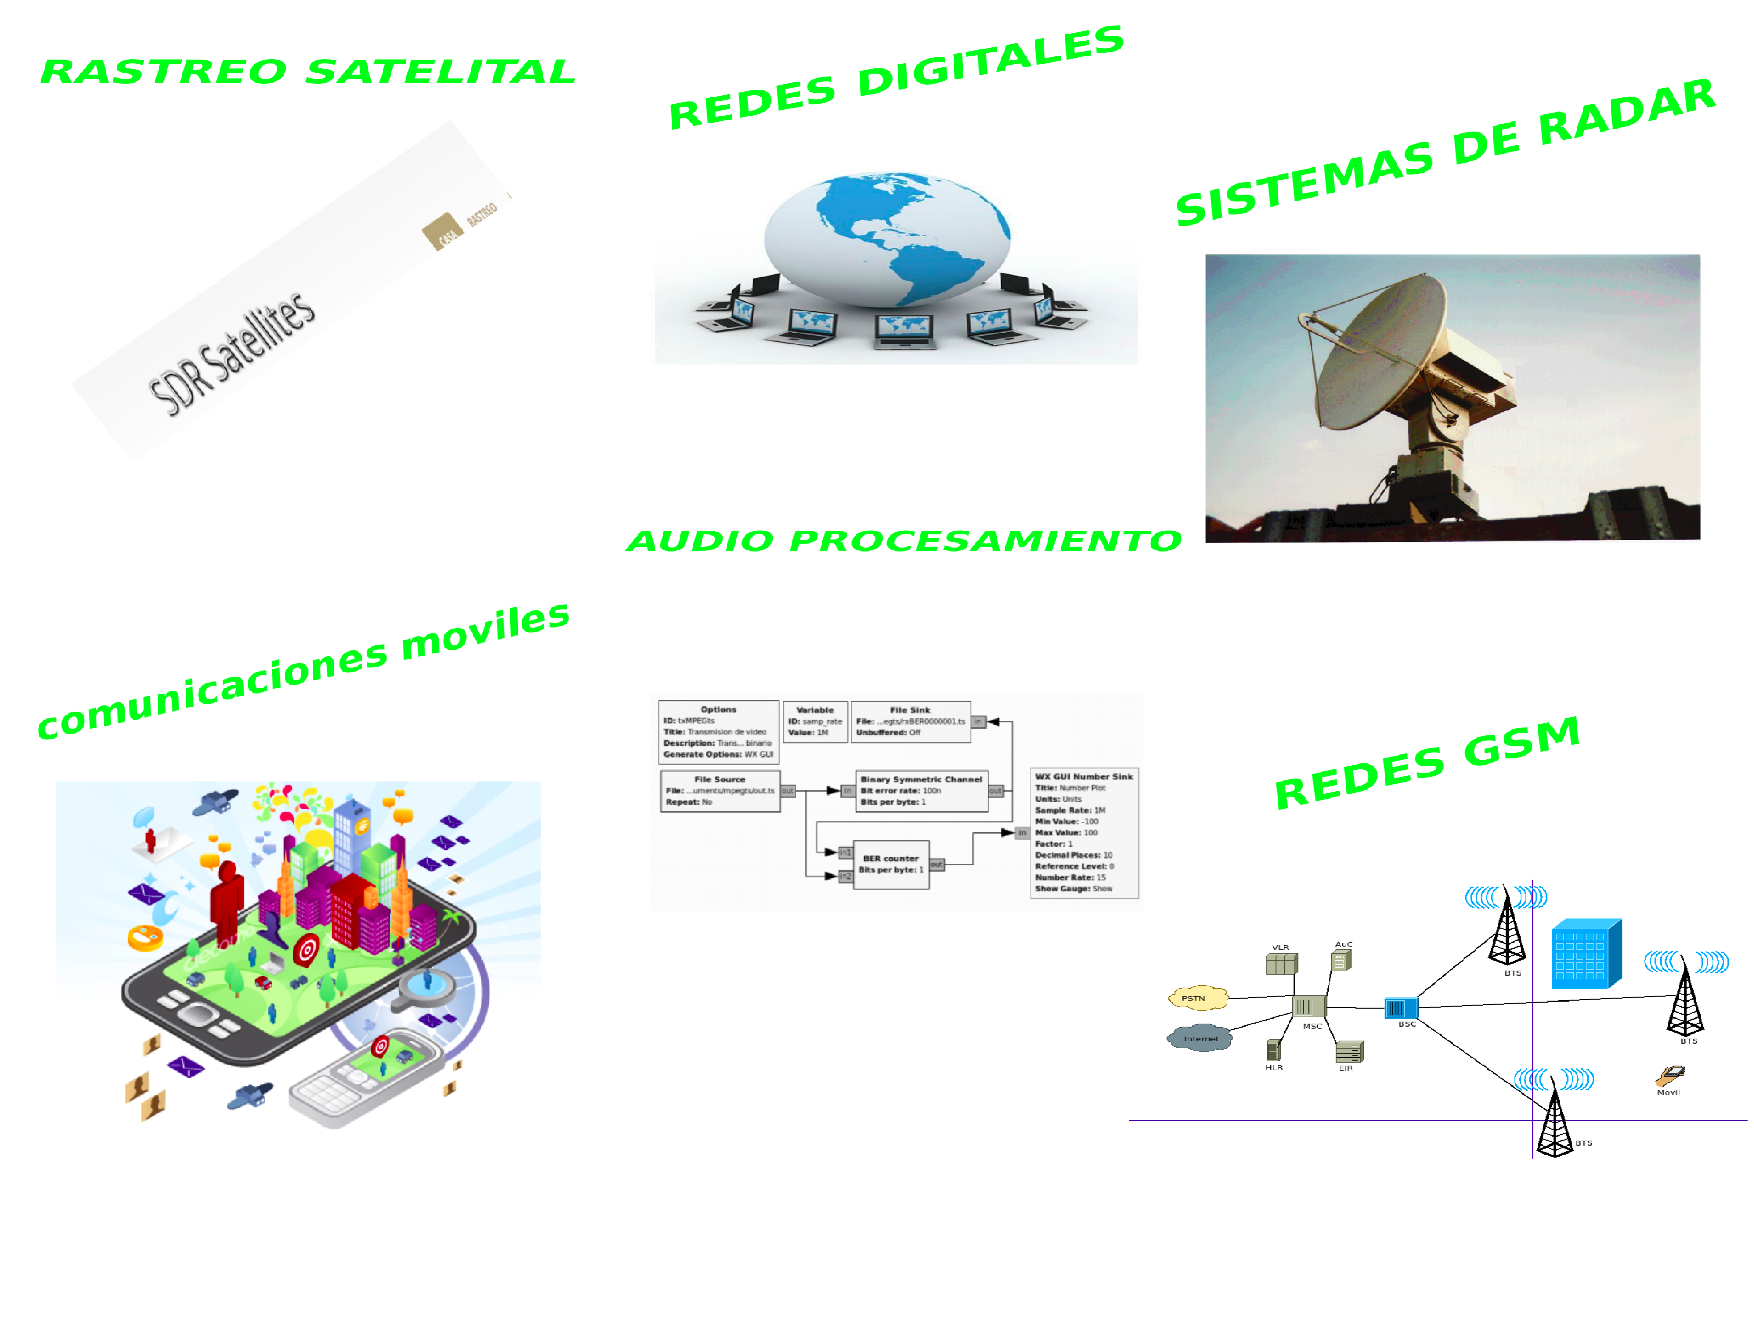
\includegraphics[width=0.9\textwidth]{parte1/intro/pdf/intro.pdf}
  \end{figure}
  
  
\end{frame}



\begin{frame}{Instalación de GNU Radio en Linux}
{Para instalar GNU Radio se deben seguir los siguientes pasos:}
\begin{enumerate}[1.]
\item Ingresar a la ventana de órdenes (o terminal) del sistema de su equipo.
\item Estando conectado a internet, escriba dentro del terminal:

  \begin{block}{}
  \texttt{
    sudo apt-get install gnuradio}
  \end{block}

\item Si su dispositivo tiene contrase\~na, debe ingresarla, al ser solicitada y oprimir \keys{\return}. 
\item Luego se deben aceptar los términos de la instalación oprimiendo la letra \keys{s} seguido de \keys{\return}. 
\item Una forma de verificar la correcta instalación es volviendo a ingresar el comando indicado en el punto 2, y si aparece un mensaje anunciando que GNU Radio ya está en su versión más reciente, su instalación fue correcta.
\end{enumerate}
\end{frame}
%----------------------------

\begin{frame}{Paquetes\index{Paquetes}}
Con el objetivo de clonar el repositorio y obtener los ejemplos de GNU Radio en nuestro ordenador se deben instalar los siguientes paquetes: 
  \begin{itemize}
  \item {BUILD-ESSENTIAL\\}
    \begin{itemize}
    \item
    {Build essential es un paquete que contiene herramientas necesarias
    para la creación, compilación e instalación de programas.}
    \end{itemize}
  \item {CMAKE\\}
  {Es un sistema de construcción de código abierto multiplataforma. Se trata de  un conjunto de herramientas diseñadas para construir, testear y empaquetar software. Se utiliza para controlar el proceso de compilación de software utilizando una plataforma sencilla y unos archivos de configuración
independientes del compilador.}
  \end{itemize}
\end{frame}
%-------------------------------

\begin{frame}{Paquetes}
  \begin{itemize}
  \item {GIT\\}
  \begin{itemize}
    \item
    {Este paquete contiene una Git; es un sistema de control de versiones distribuidas de código abierto desarrollado originalmente por Linux Torvalds para apoyar el desarrollo del kernel de Linux.}
    \item
    {El control de versiones es un sistema que registra los cambios realizados sobre un archivo o conjunto de archivos a lo largo del tiempo, de modo que se puedan recuperar versiones específicas más adelante.}
    \end{itemize}
  \item {LIBBOOST-ALL-DEV\\}
  {Es una biblioteca de software libre y revisión por partes preparadas para extender las capacidades del lenguaje de programación; permite ser utilizada en cualquier tipo de proyectos.}
  \end{itemize}
\end{frame}

%++++++++++++++++++++

\begin{frame}{Paquetes\index{Paquetes}}
  \begin{itemize}
  \item {LIBCPPUNIT-DEV\\}
  \begin{itemize}
    \item
    {Biblioteca de pruebas unitarias para C++.}
    \item
    {Una prueba unitaria es una forma de comprobar el correcto
funcionamiento de una unidad de código. Por ejemplo, en diseño
estructurado o en diseño funcional, una función o un procedimiento,
en diseño orientado a objetos una clase. Esto sirve para asegurar que
cada unidad funcione correcta y eficientemente por separado.}
    \end{itemize}
  \item {DOXYGEN\\}
  {Es una herramienta para generar documentación a partir de código fuente. Es un sistema de documentación para C++, C, Java, Python. Es necesario solo si se desea generar referencias a documentación externa de la que no tiene las fuentes.}
  \end{itemize}
\end{frame}

%+++++++++++++++++++

\begin{frame}{Instalación de paquetes}
\begin{enumerate}[1.]
\item La instalación de cada uno se los paquetes anteriormente mencionados, se realiza colocando, en la ventana de terminal, las siguientes órdenes:
\end{enumerate}

  \begin{block}{}
  \texttt{
  \ \ \ sudo apt-get install build-essential
    \begin{itemize}
      \item[] sudo apt-get install cmake
      \item[] sudo apt-get install git
      \item[] sudo apt-get install libboost-all-dev
      \item[] sudo apt-get install libcppunit-dev
      \item[] sudo apt-get install doxygen
    \end{itemize}}
  \end{block}


\end{frame}

%++++++++++++++++++++


\begin{frame}{Clonar repositorio\index{Clonar Repositorio}}
El código fuente de los ejemplos está almacenado en github por lo tanto para clonar el repositorio se debe realizar lo siguiente:
\begin{itemize}
\item Abrir la ventana de órdenes o terminal.
\item Después se debe ingresar el siguiente comando para clonar el directorio git:

\begin{block}{}
  \texttt{
    git clone https://github.com/gnuradio/gr-tutorial}
  \end{block}

\item Una vez clonado el directorio se deben ver exactamente los mismos archivos y carpetas que los del repositorio github, en el PC empleado.
\end{itemize}
\end{frame}

%+++++++++++++++++++

\begin{frame}{Instalación de módulos\index{Modulos}}
\begin{itemize}
\item Luego de haber clonado el repositorio, debemos buscar la carpeta de gr-tutorial e ingresar a ella desde el terminal, para ello se digitan los siguientes mandos:

  \begin{block}{}
  \texttt{
  \ \ \ ls
    \begin{itemize}
      \item[] cd gr-tutorial
    \end{itemize}}
  \end{block}

Es importante mencionar que al escribir el primer comando se podrán observar la diferentes carpetas que se encuentran en el dispositivo, por lo tanto gr-tutorial debe aparecer entre las opciones para poder cambiar de directorio. 
\end{itemize}
\end{frame}

%+++++++++++++++

\begin{frame}{Instalación de módulos\index{Modulos}}
\begin{itemize}
\item Estando dentro de la carpeta, desde la terminal, se deben escribir los siguientes comandos, con la finalidad de instalar las soluciones o módulos:

  \begin{block}{}
  \texttt{
  \ \ \ mkdir build
    \begin{itemize}
      \item[] cd build
      \item[] cmake ..
      \item[] make -j8
      \item[] sudo make install
      \item[]sudo ldconfig
    \end{itemize}}
  \end{block}

\end{itemize}
\end{frame}


%///////////////////////////////////////////////////////////////

\subsection{Lab1: Primeros pasos}
%*********************
\begin{frame}{}

\pgfdeclareimage[width=\paperwidth,height=\paperheight]{bg}{imagenes/fondo_lab}
\setbeamertemplate{background}{\pgfuseimage{bg}}

\bfseries{\textrm{\LARGE Lab1\\ \Large Primeros pasos}}
\raggedright
\end{frame}
%*********************

\begin{frame}{Primeros pasos}

\pgfdeclareimage[width=\paperwidth,height=\paperheight]{bg}{imagenes/fondo3}
\setbeamertemplate{background}{\pgfuseimage{bg}}

\begin{figure}[H]
\centering
\vspace{-3mm}
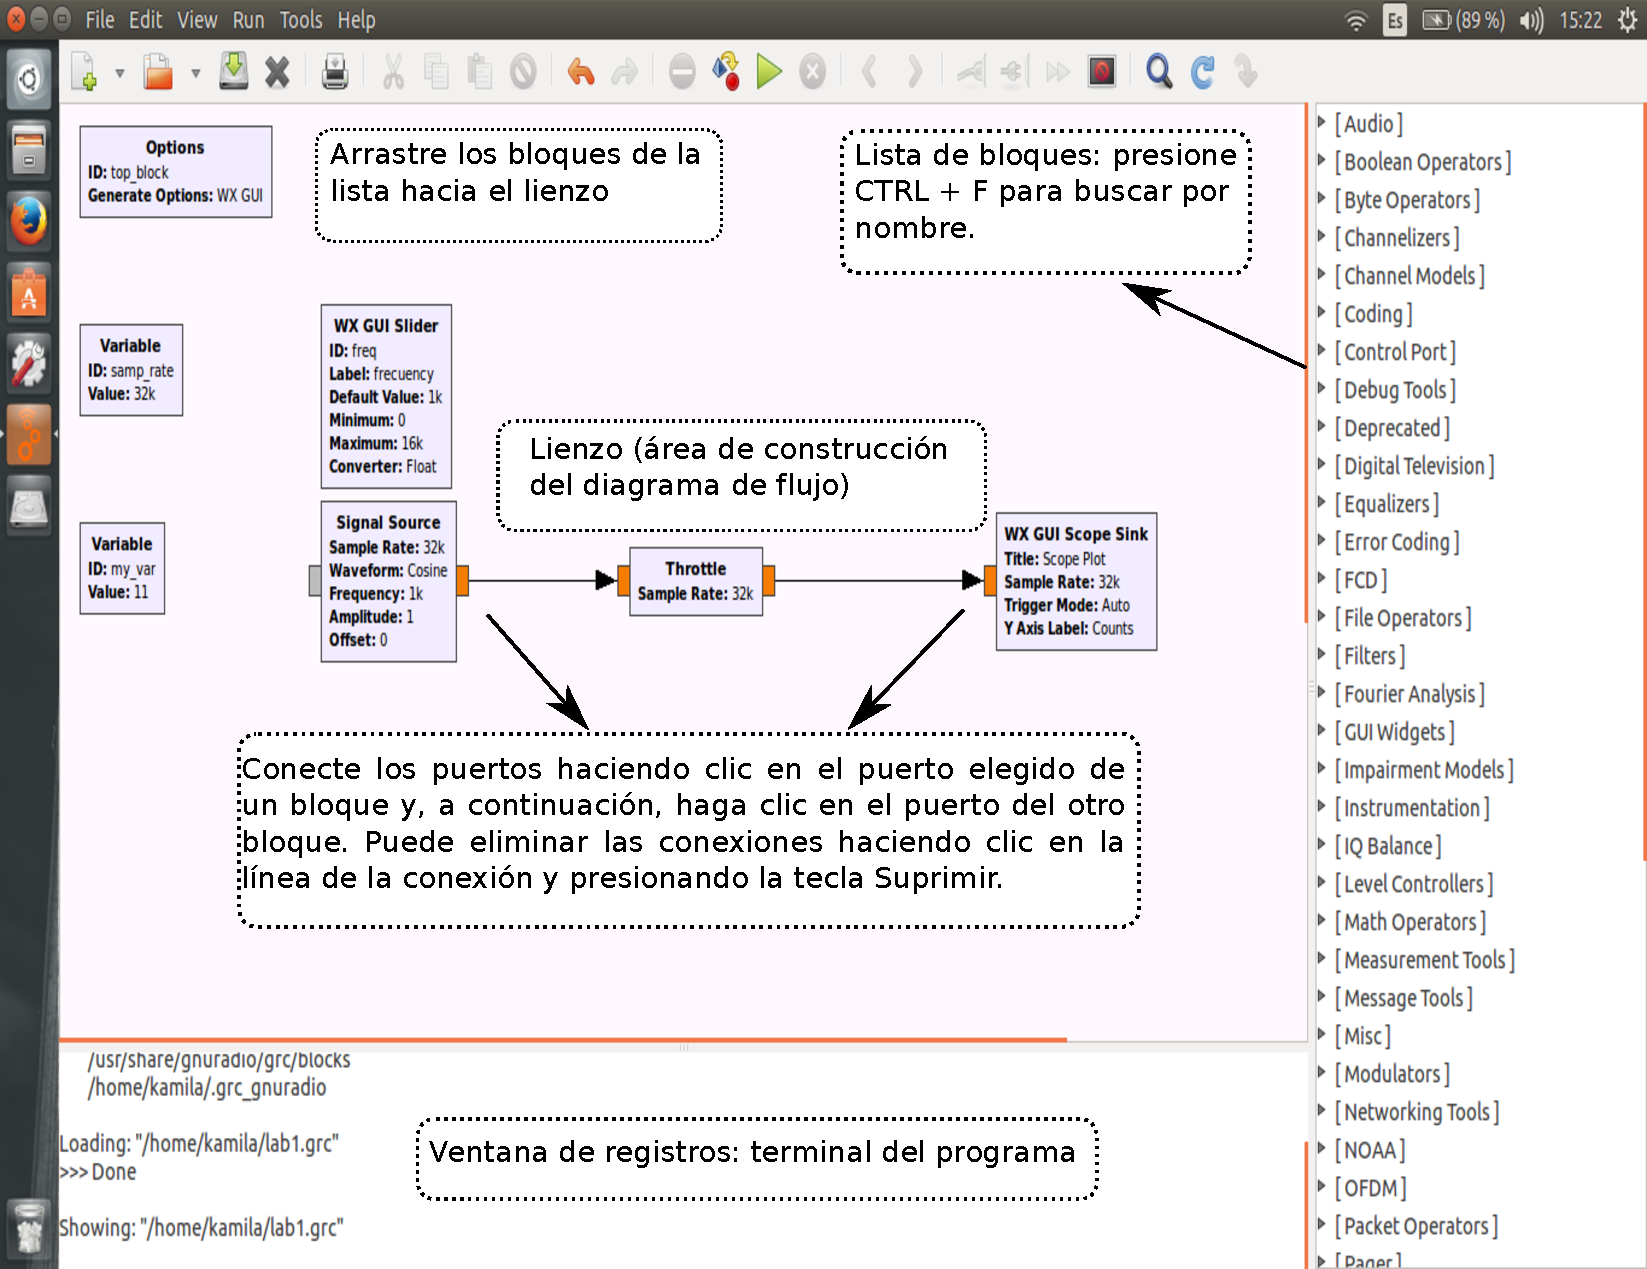
\includegraphics[width=0.9\textwidth]{parte1/lab1/pdf/lab1_1.pdf}
\end{figure}
\end{frame}
%-----------------------------------

\begin{frame}{Primeros pasos }
\begin{figure}[H]
\centering
\vspace{-3mm}
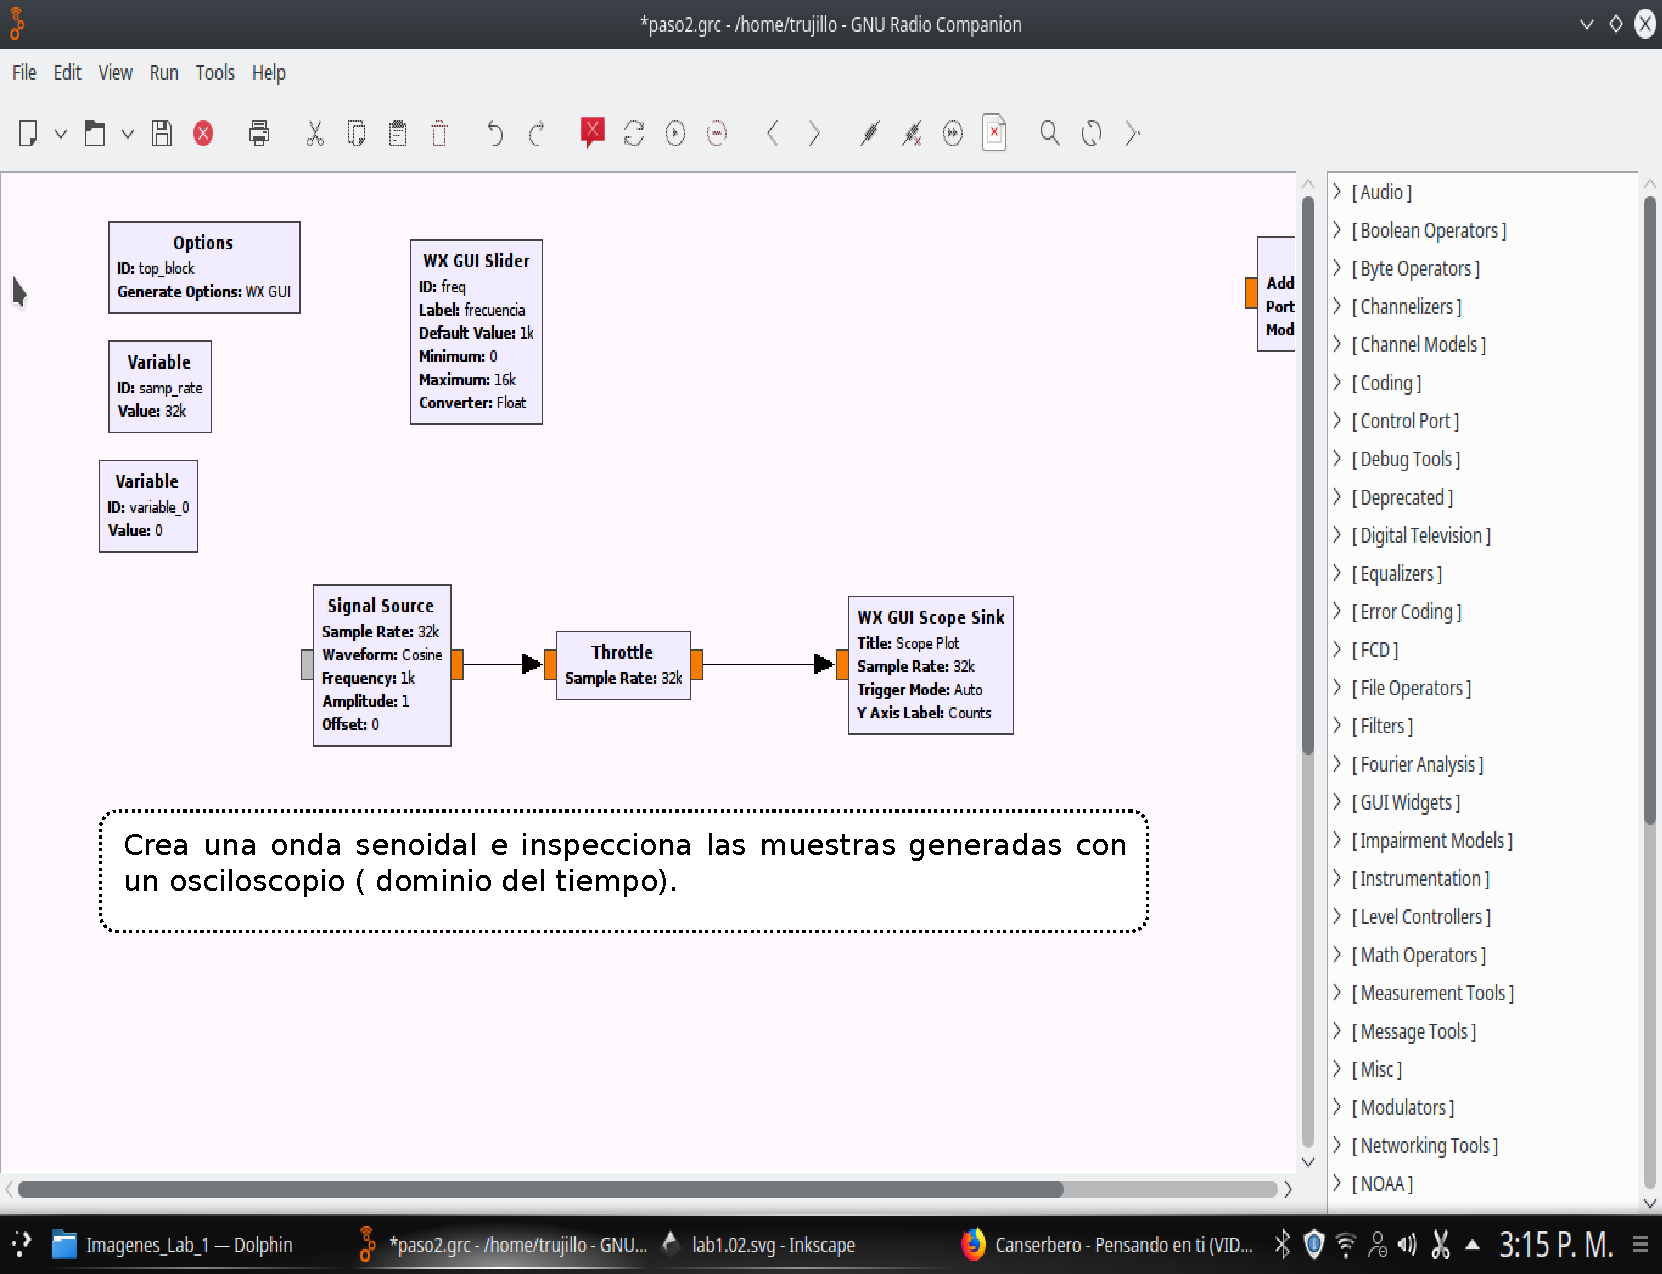
\includegraphics[width=0.9\textwidth]{parte1/lab1/pdf/lab1_2.pdf}
\end{figure}
\end{frame}
%-----------------------------------

\begin{frame}{Primeros pasos }
\begin{figure}[H]
\vspace{-3mm}
\centering
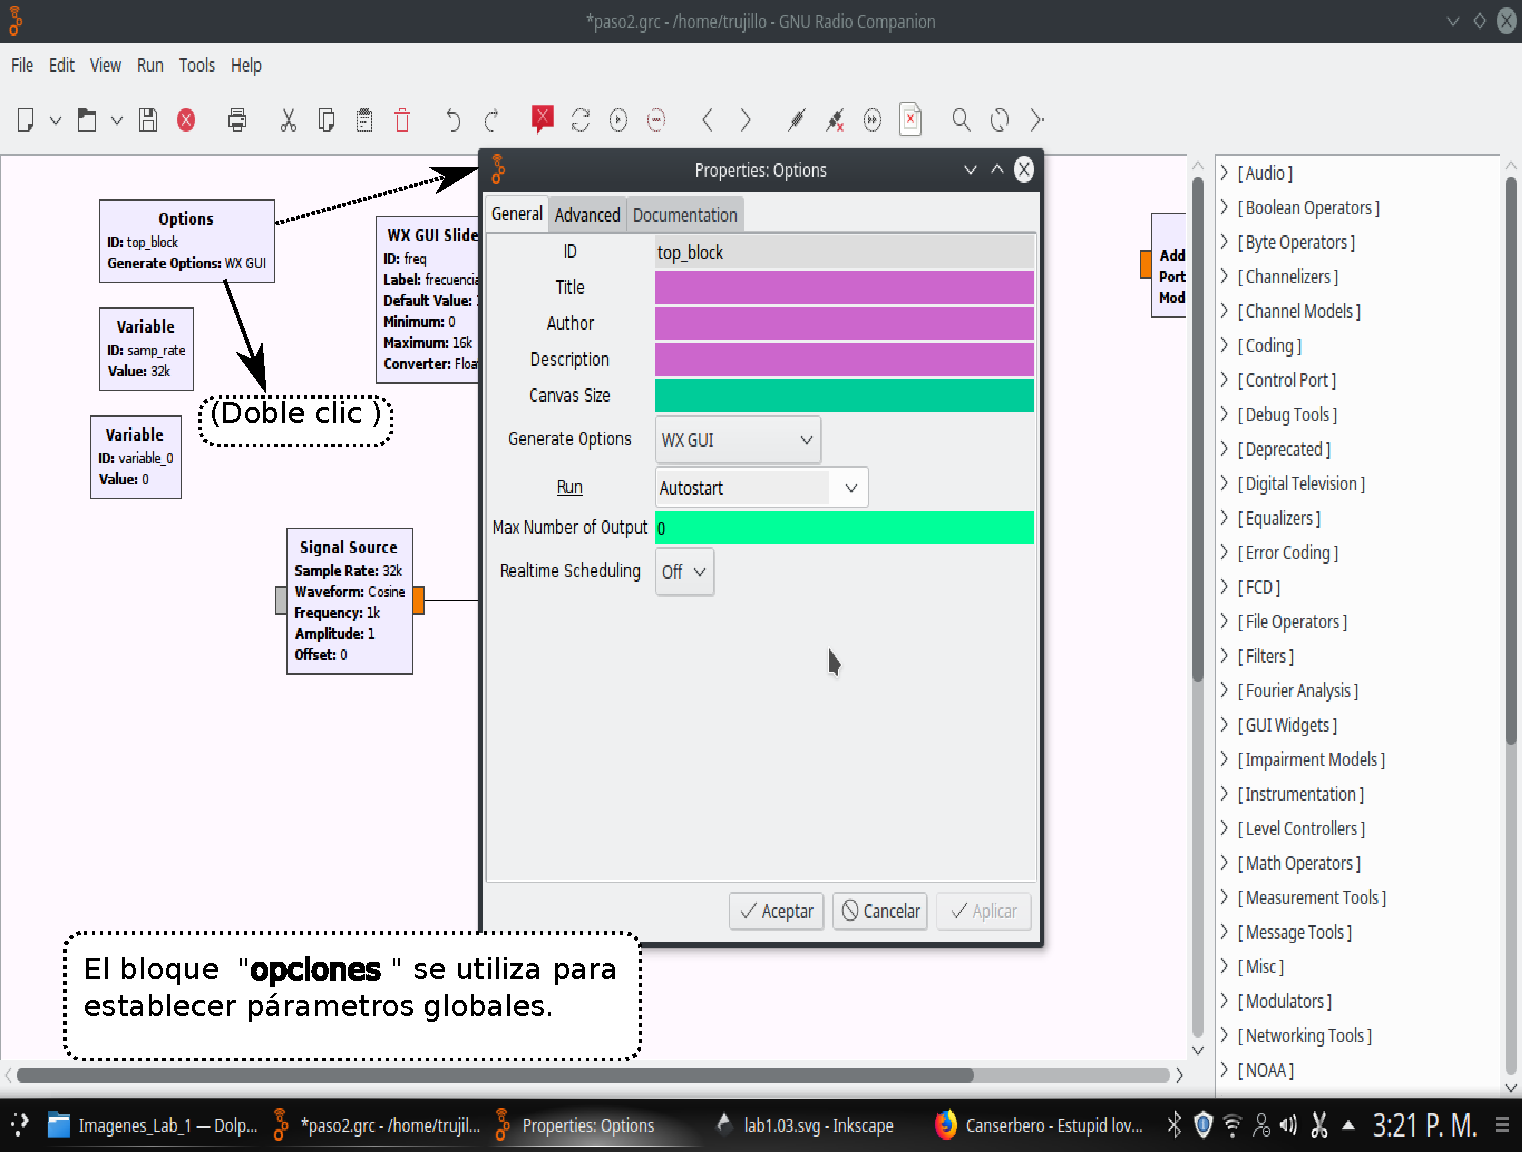
\includegraphics[width=0.9\textwidth]{parte1/lab1/pdf/lab1_3.pdf}
\end{figure}
\end{frame}
%-----------------------------------

\begin{frame}{Primeros pasos }
\begin{figure}[H]
\vspace{-3mm}
\centering
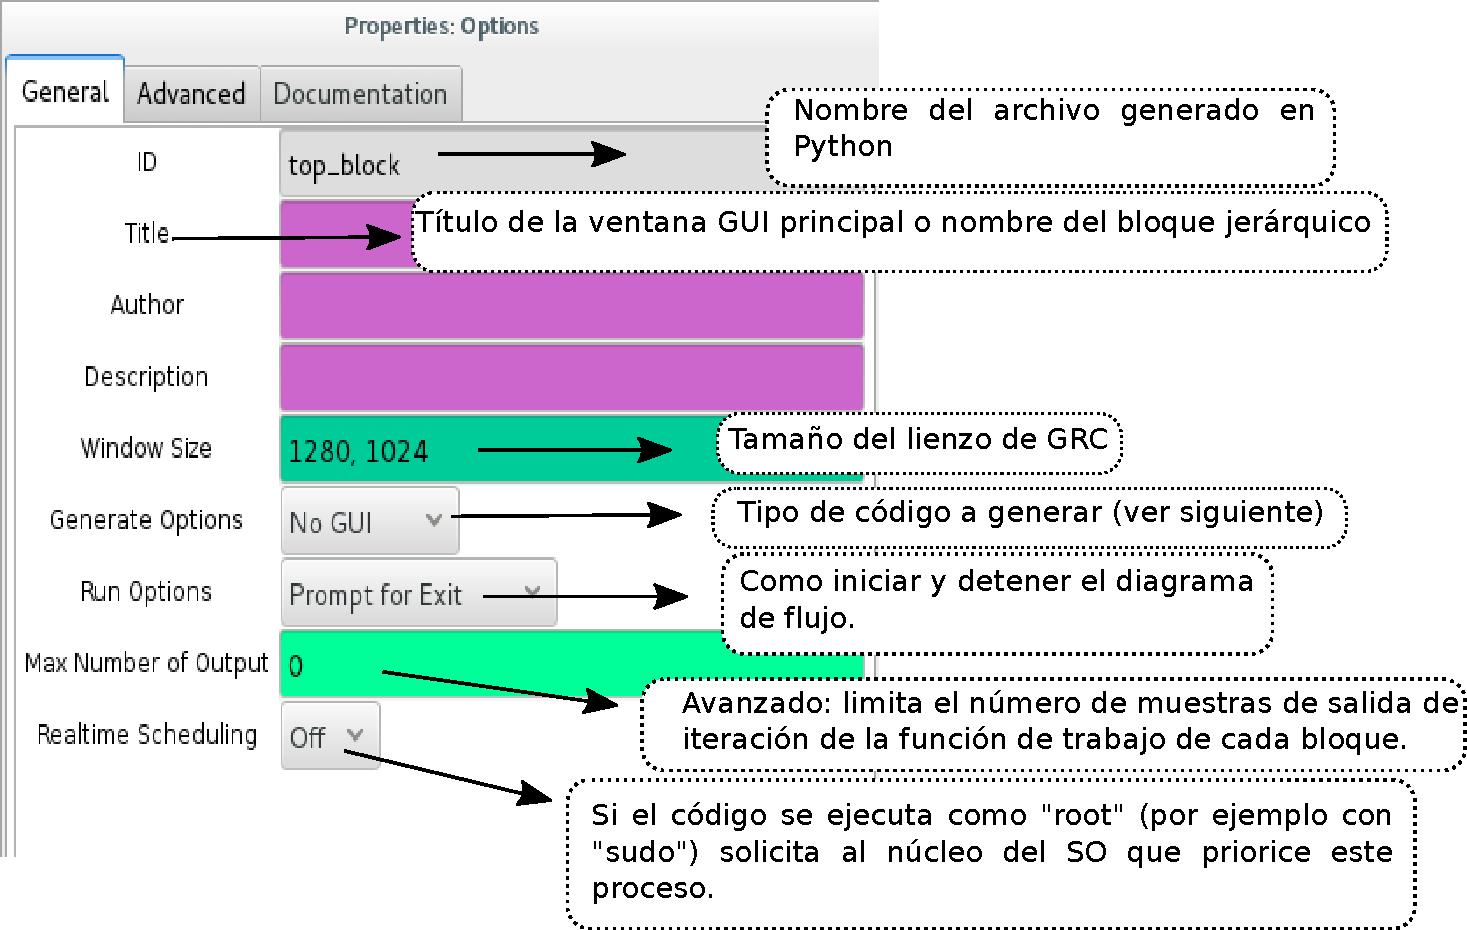
\includegraphics[width=0.9\textwidth]{parte1/lab1/pdf/lab1_4.pdf}
\end{figure}
\end{frame}
%-----------------------------------

\begin{frame}{Primeros pasos }
\begin{figure}[H]
\vspace{-2cm}
\centering
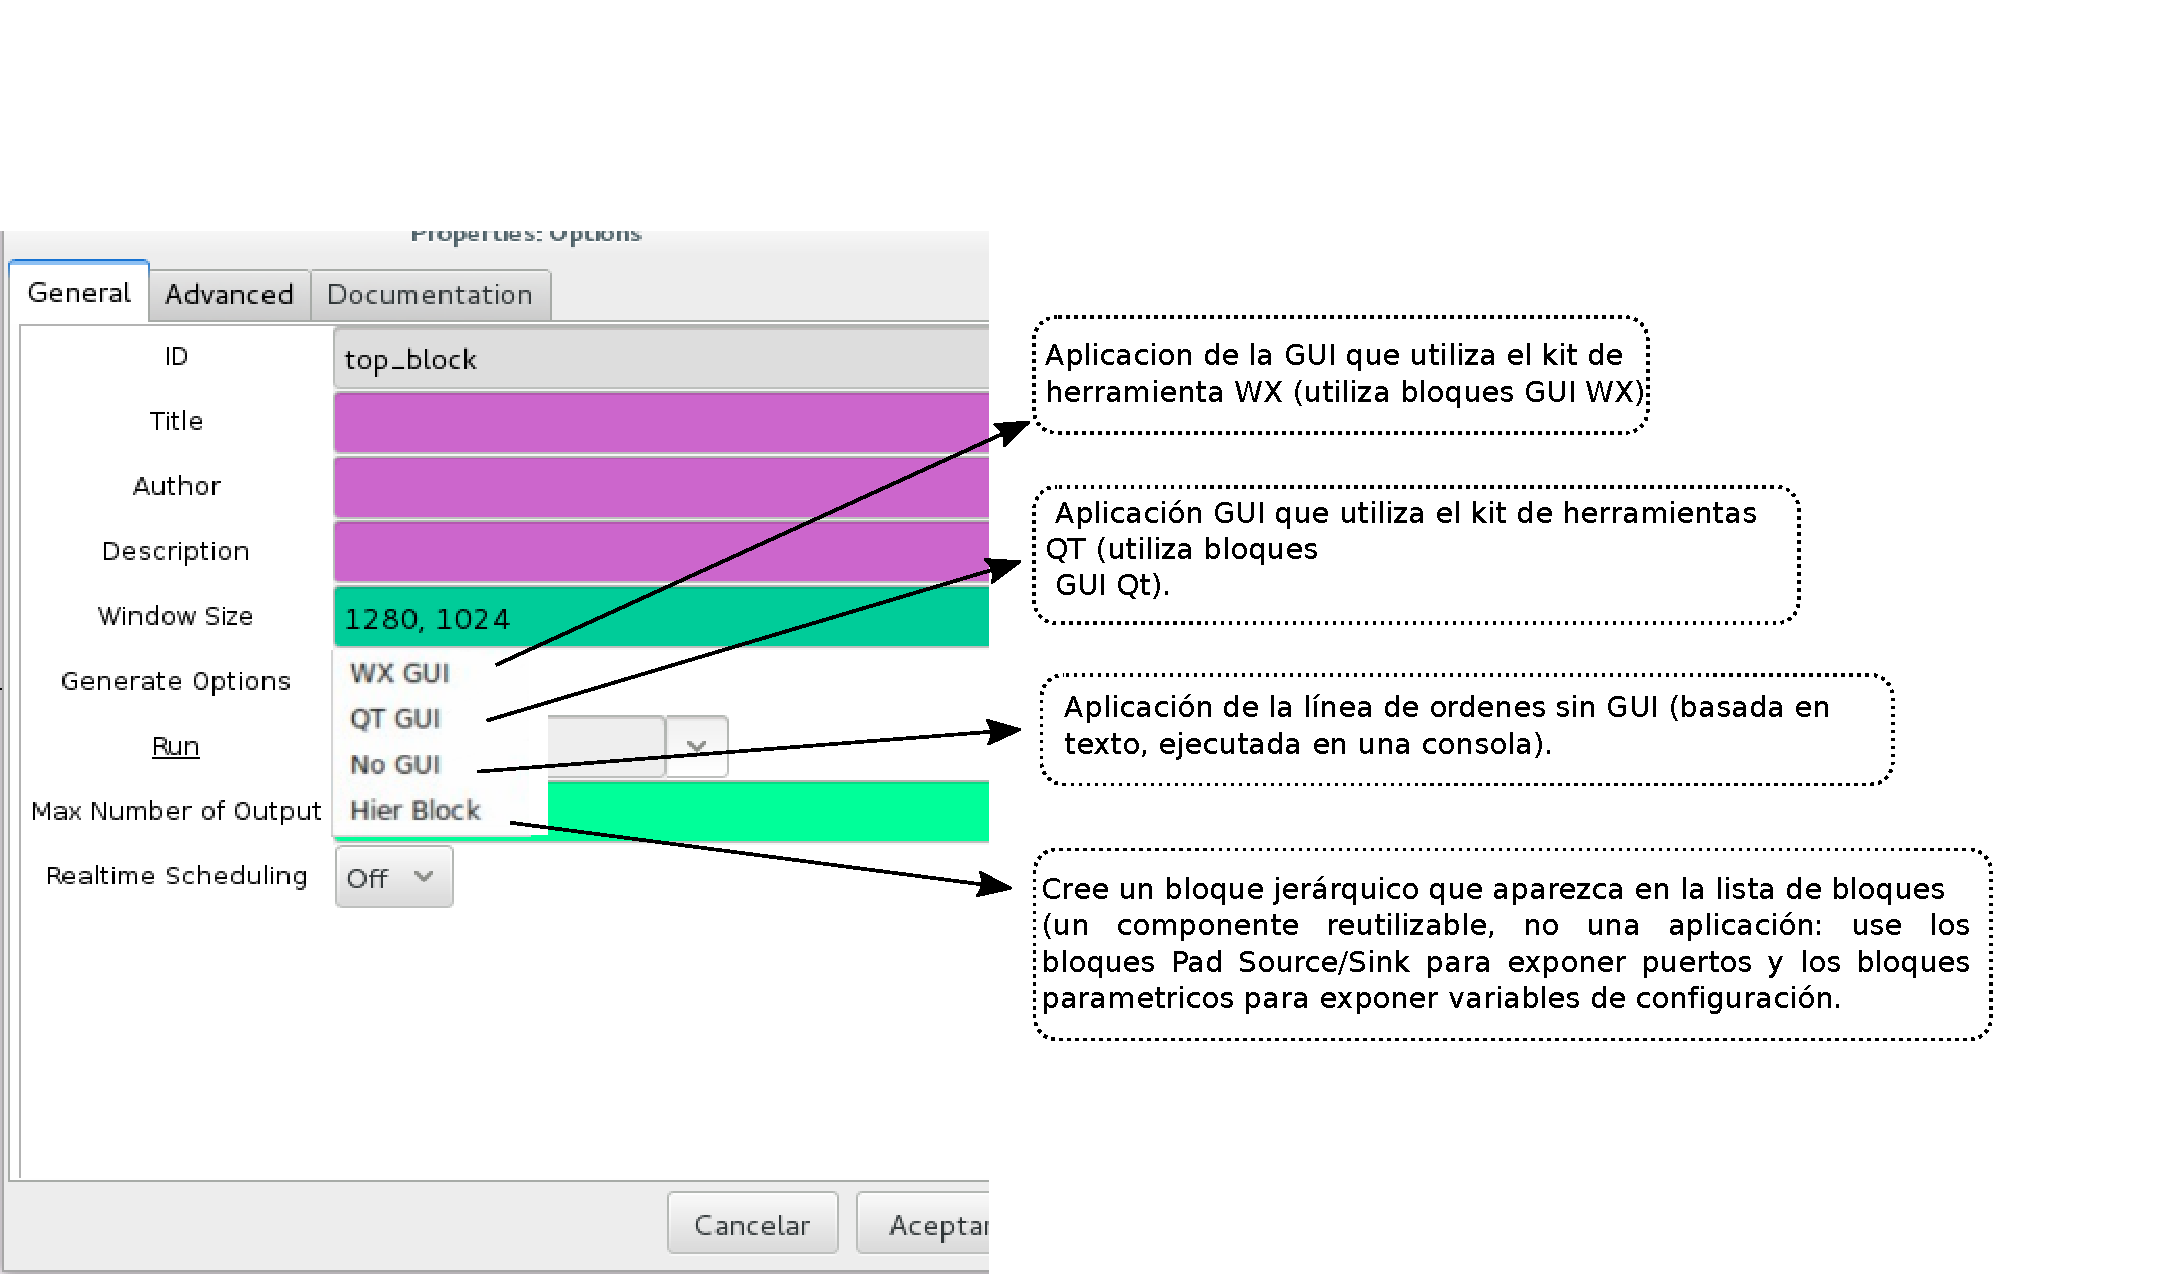
\includegraphics[width=1.1\textwidth]{parte1/lab1/pdf/lab1_5.pdf}
\end{figure}
\end{frame}
%-----------------------------------

\begin{frame}{Primeros pasos }
\begin{figure}[H]
\centering
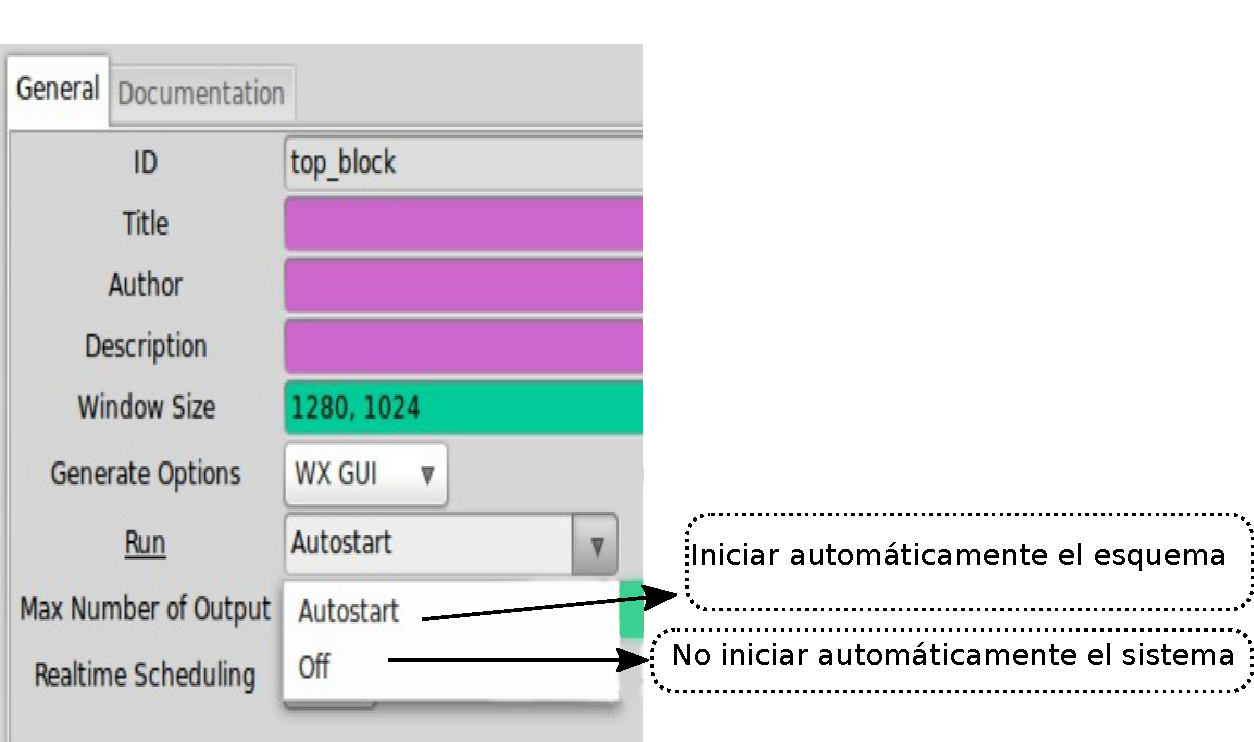
\includegraphics[width=.9\textwidth]{parte1/lab1/pdf/lab1_6.pdf}
\end{figure}
\end{frame}
%-----------------------------------

\begin{frame}{Primeros pasos }
\begin{figure}[H]
\centering
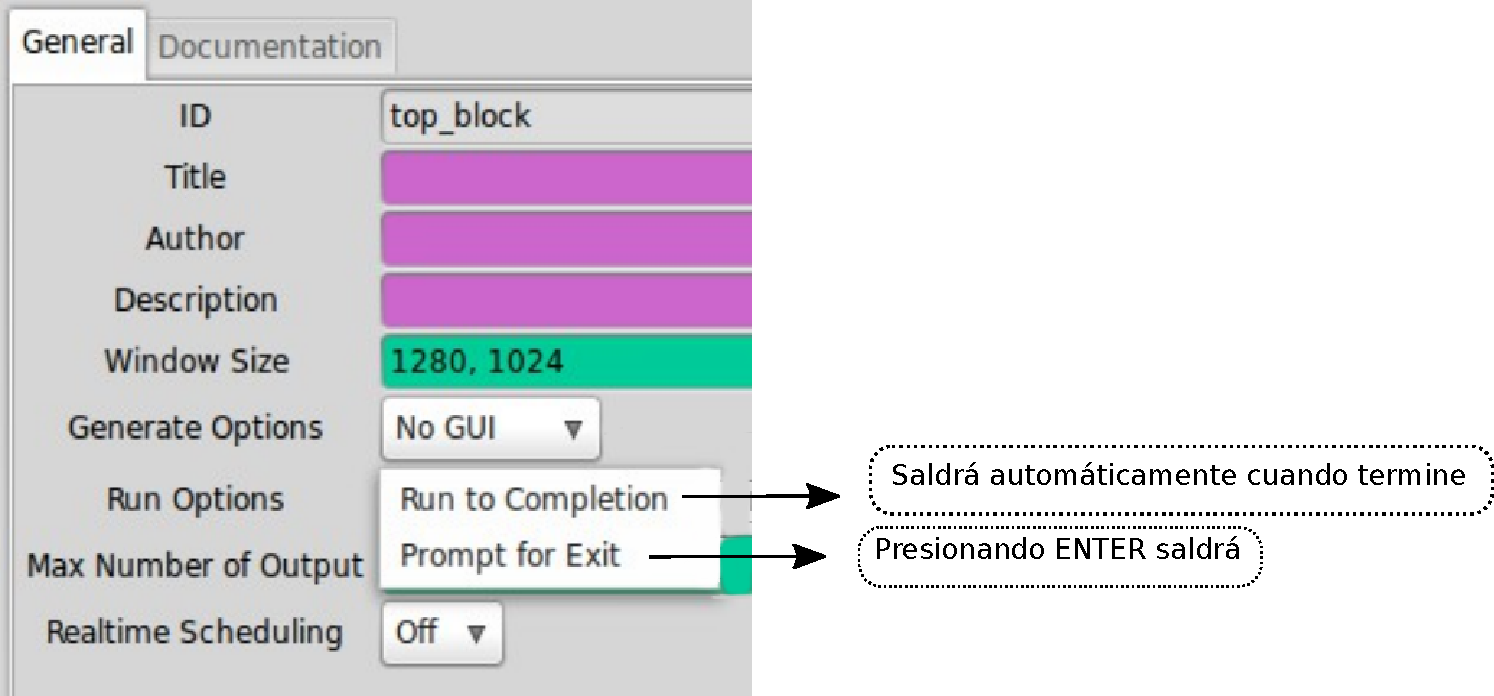
\includegraphics[width=\textwidth]{parte1/lab1/pdf/lab1_7.pdf}
\end{figure}
\end{frame}
%-----------------------------------

\begin{frame}{Primeros pasos }
\begin{figure}[H]
\vspace{-1cm}
\centering
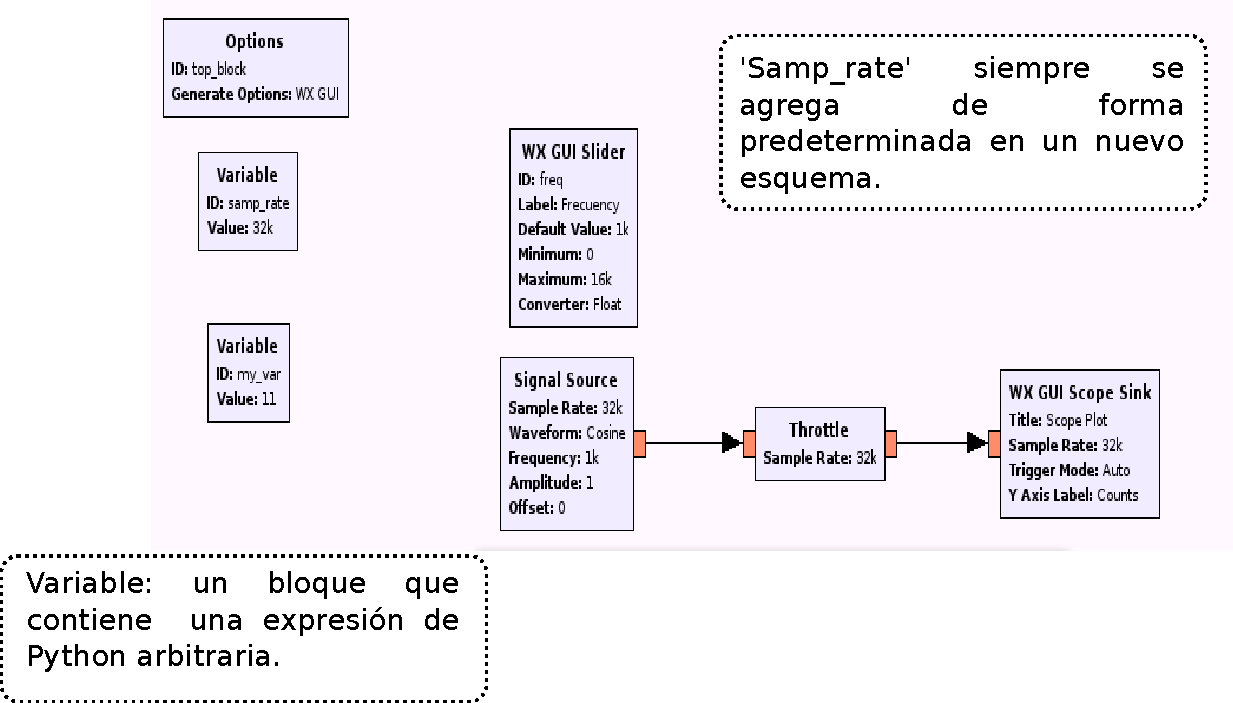
\includegraphics[width=\textwidth]{parte1/lab1/pdf/lab1_8.pdf}
\end{figure}
\end{frame}
%-----------------------------------

\begin{frame}{Primeros pasos }
\begin{figure}[H]
\vspace{-3mm}
\centering
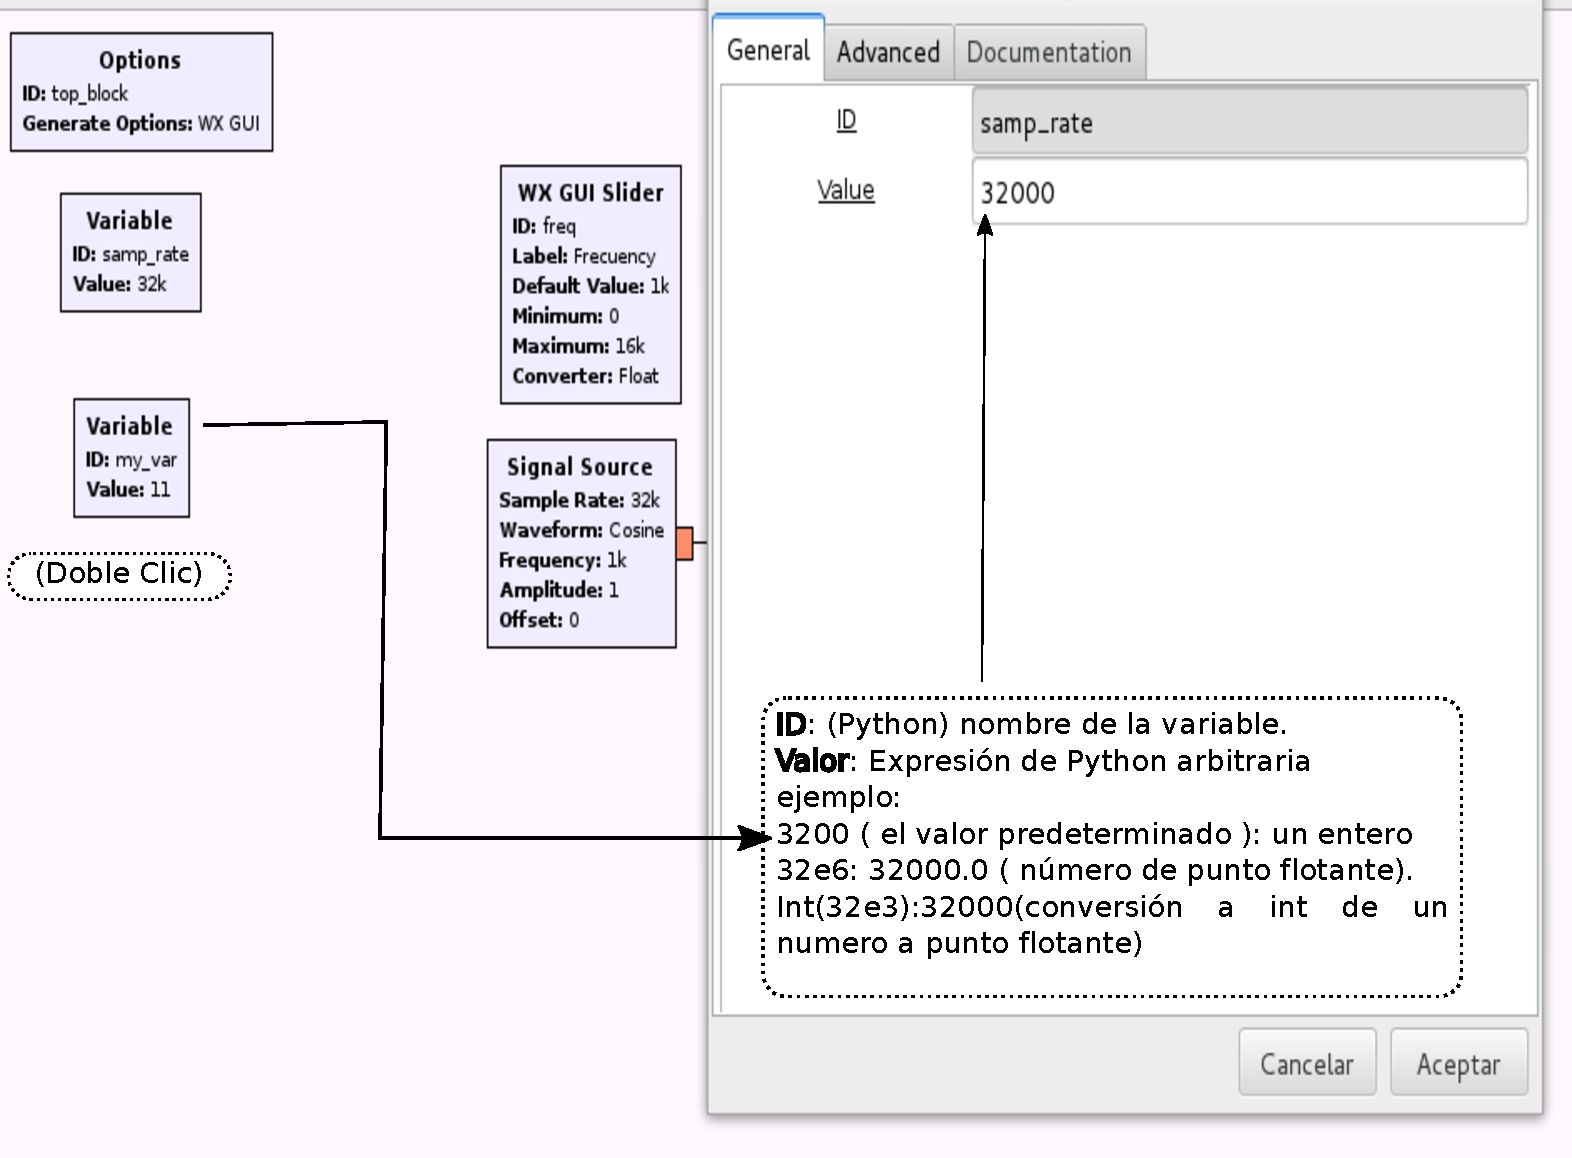
\includegraphics[width=0.85\textwidth]{parte1/lab1/pdf/lab1_9.pdf}
\end{figure}
\end{frame}
%-----------------------------------

\begin{frame}{Primeros pasos }
\begin{figure}[H]
\vspace{-3mm}
\centering
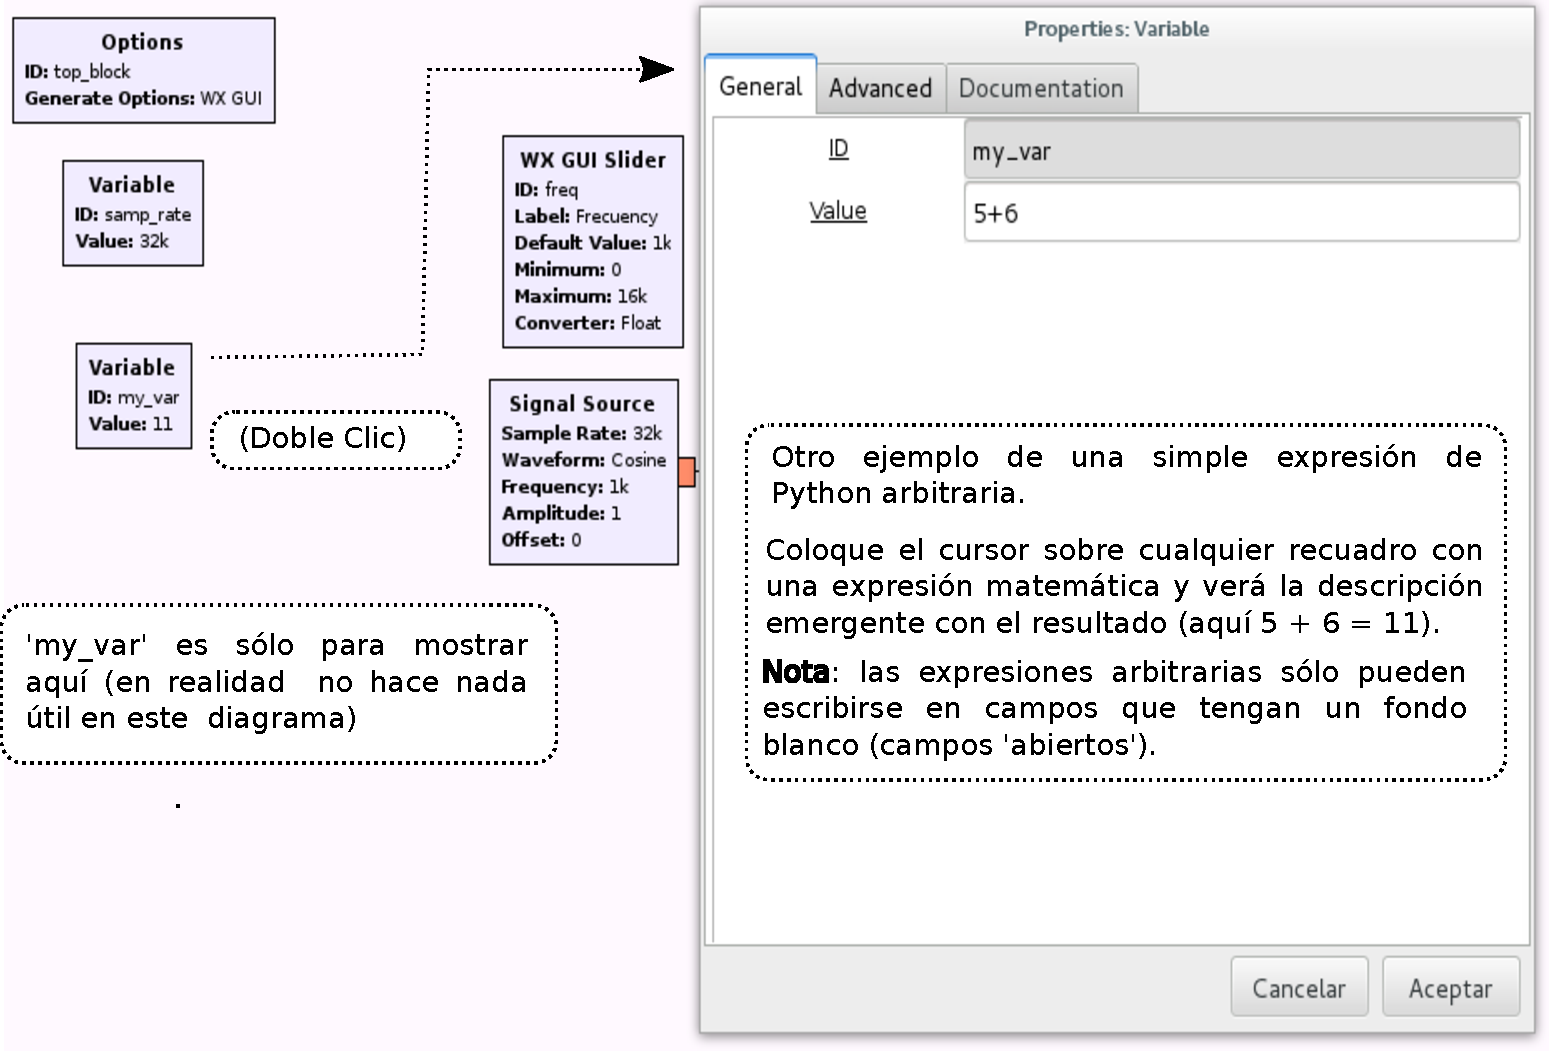
\includegraphics[width=.9\textwidth]{parte1/lab1/pdf/lab1_10.pdf}
\end{figure}
\end{frame}
%-----------------------------------

\begin{frame}{Primeros pasos }
\begin{figure}[H]
\vspace{-3mm}
\centering
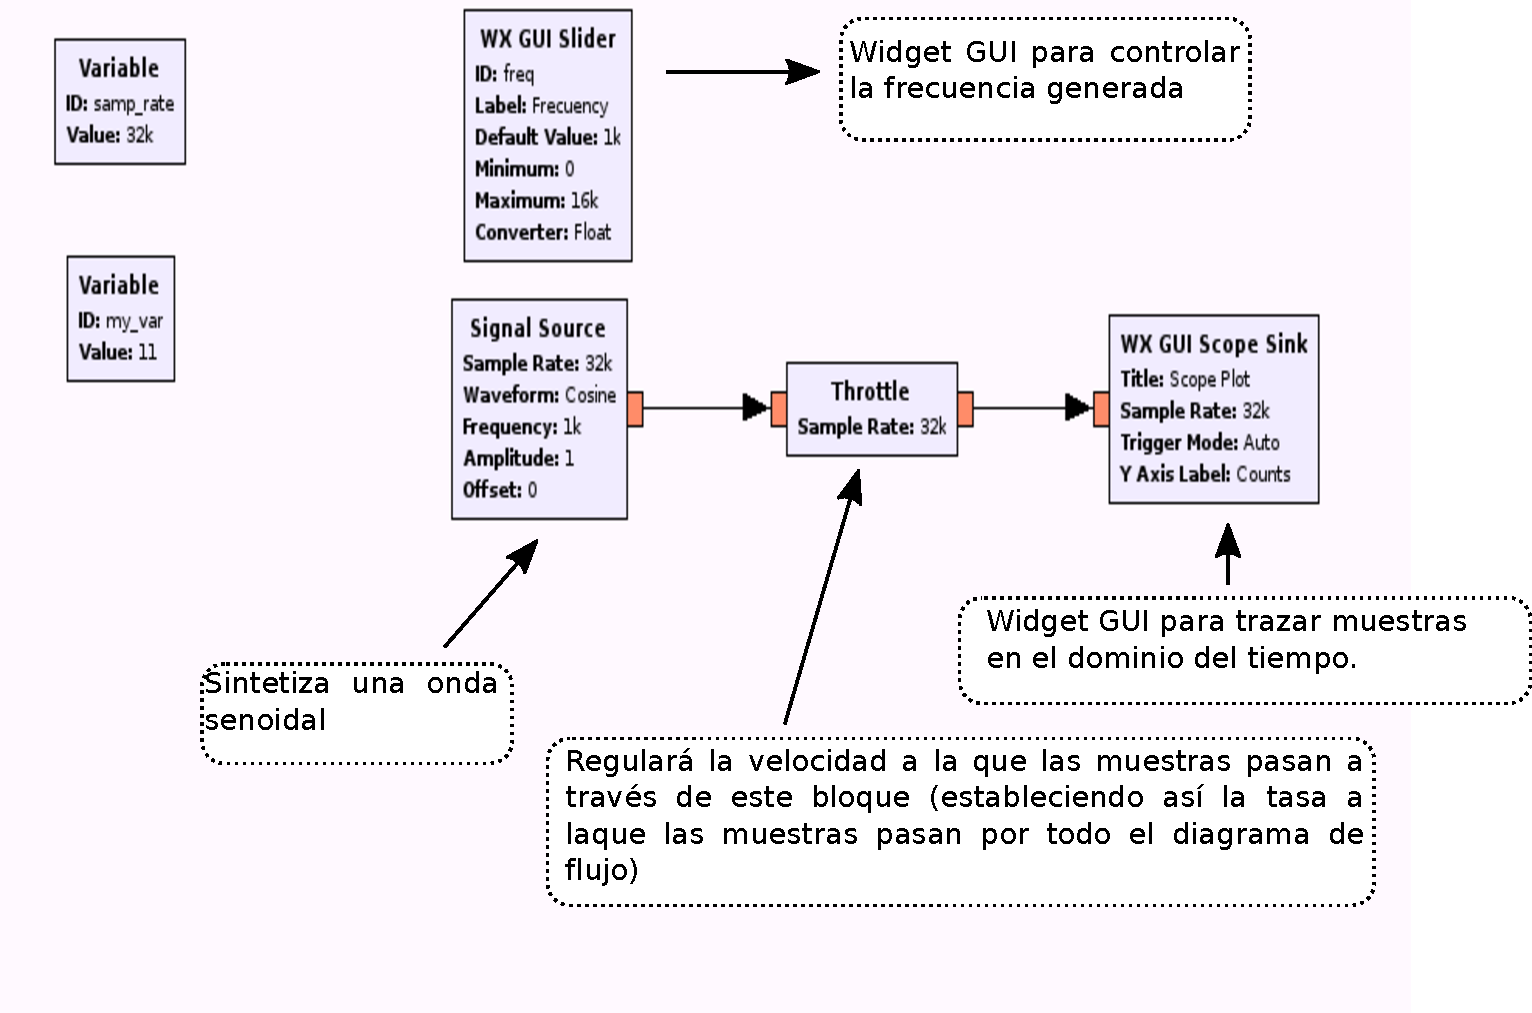
\includegraphics[width=\textwidth]{parte1/lab1/pdf/lab1_11.pdf}
\end{figure}
\end{frame}
%-----------------------------------

\begin{frame}{Primeros pasos }
\begin{figure}[H]
\vspace{-3mm}
\centering
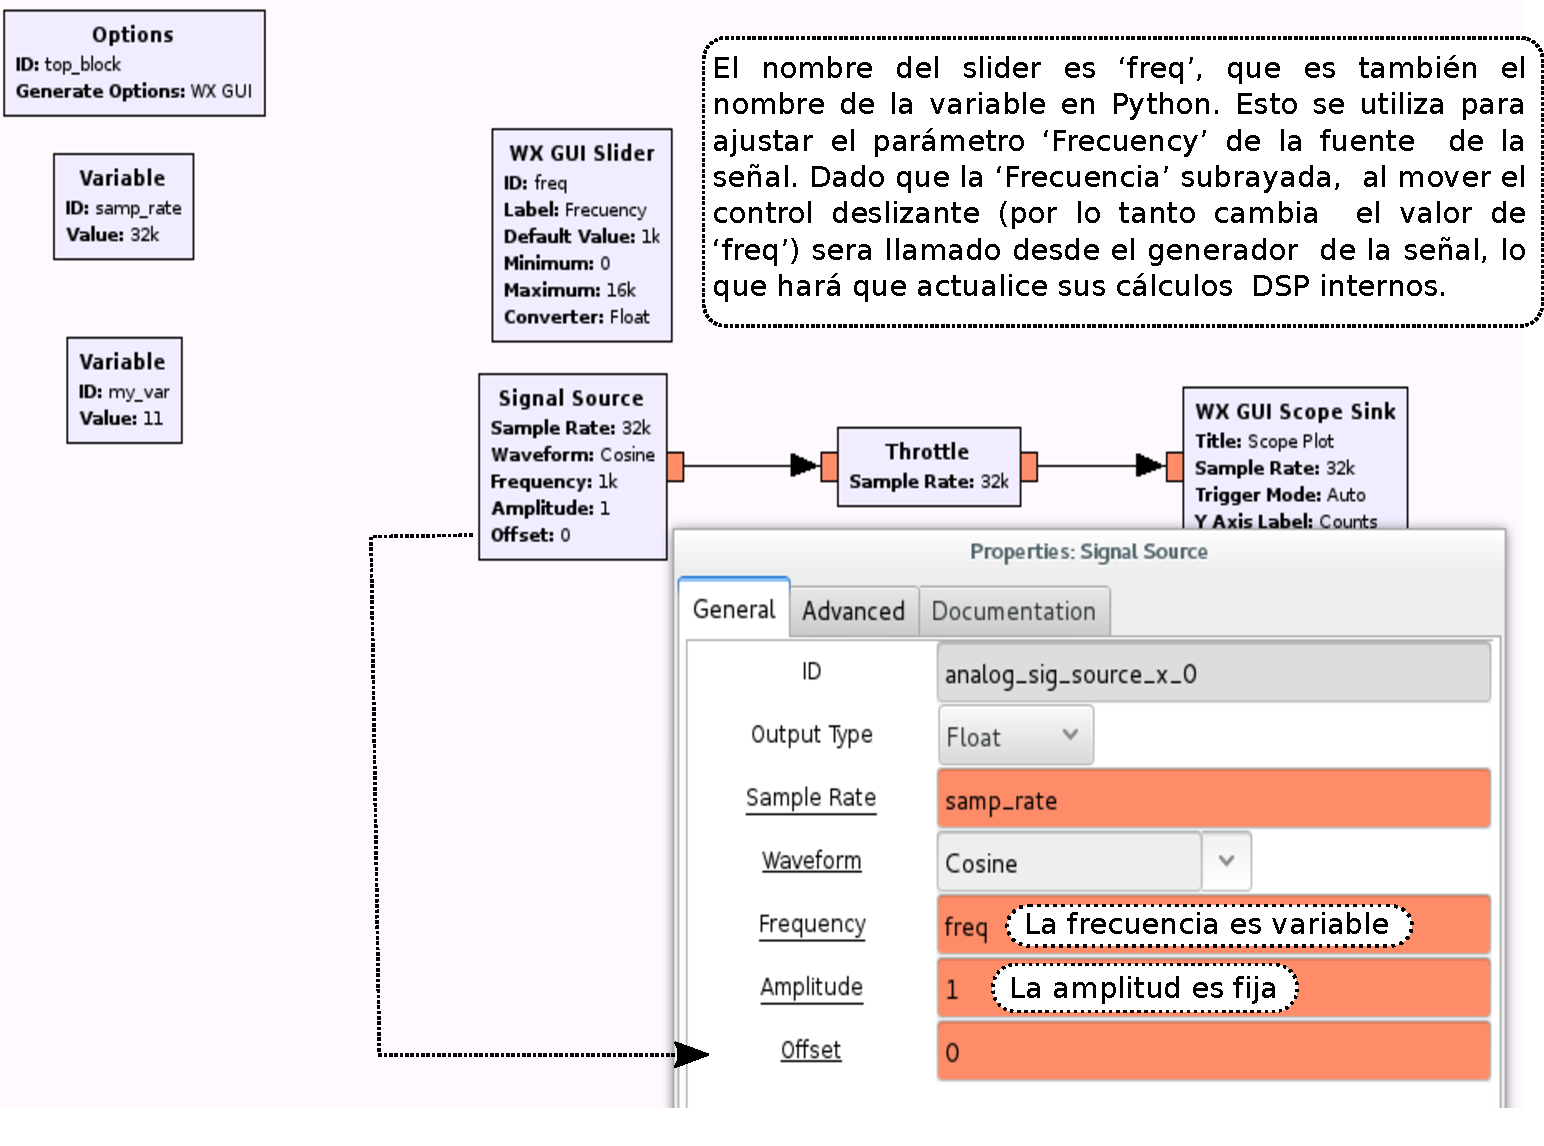
\includegraphics[width=.85\textwidth]{parte1/lab1/pdf/lab1_12.pdf}
\end{figure}
\end{frame}
%-----------------------------------

\begin{frame}{Primeros pasos }
\begin{figure}[H]
\vspace{-3mm}
\centering
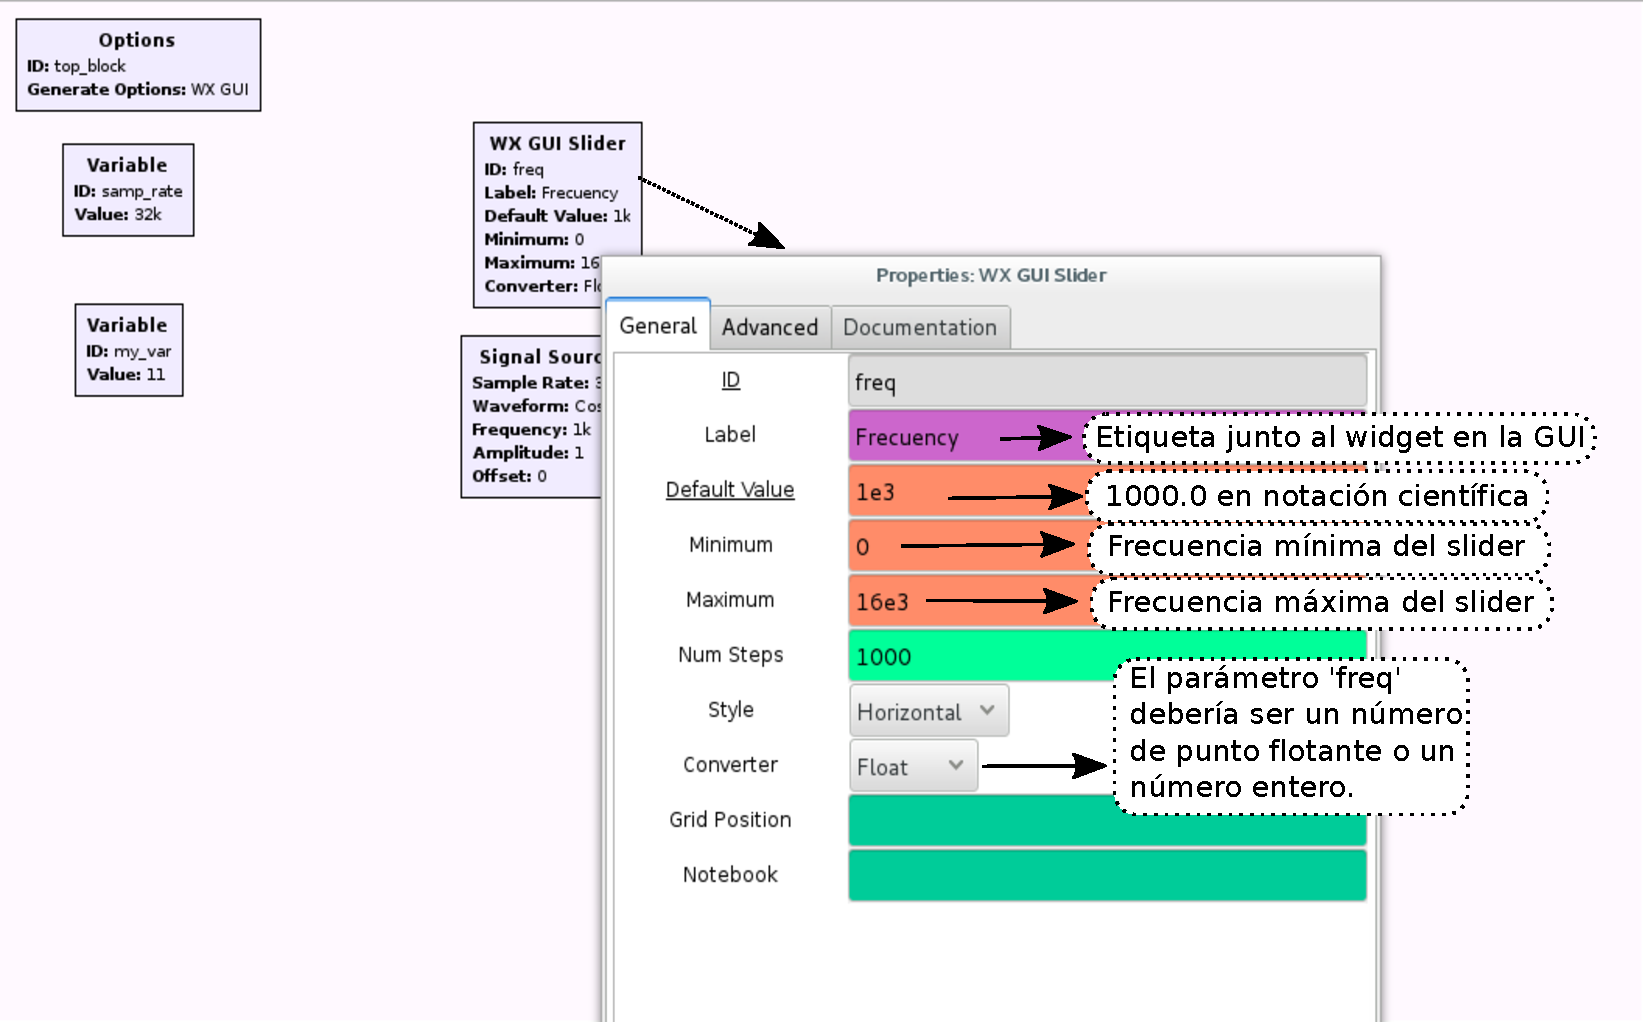
\includegraphics[width=\textwidth]{parte1/lab1/pdf/lab1_13.pdf}
\end{figure}
\end{frame}
%-----------------------------------

\begin{frame}{Primeros pasos }
\begin{figure}[H]
\vspace{-1cm}
\centering
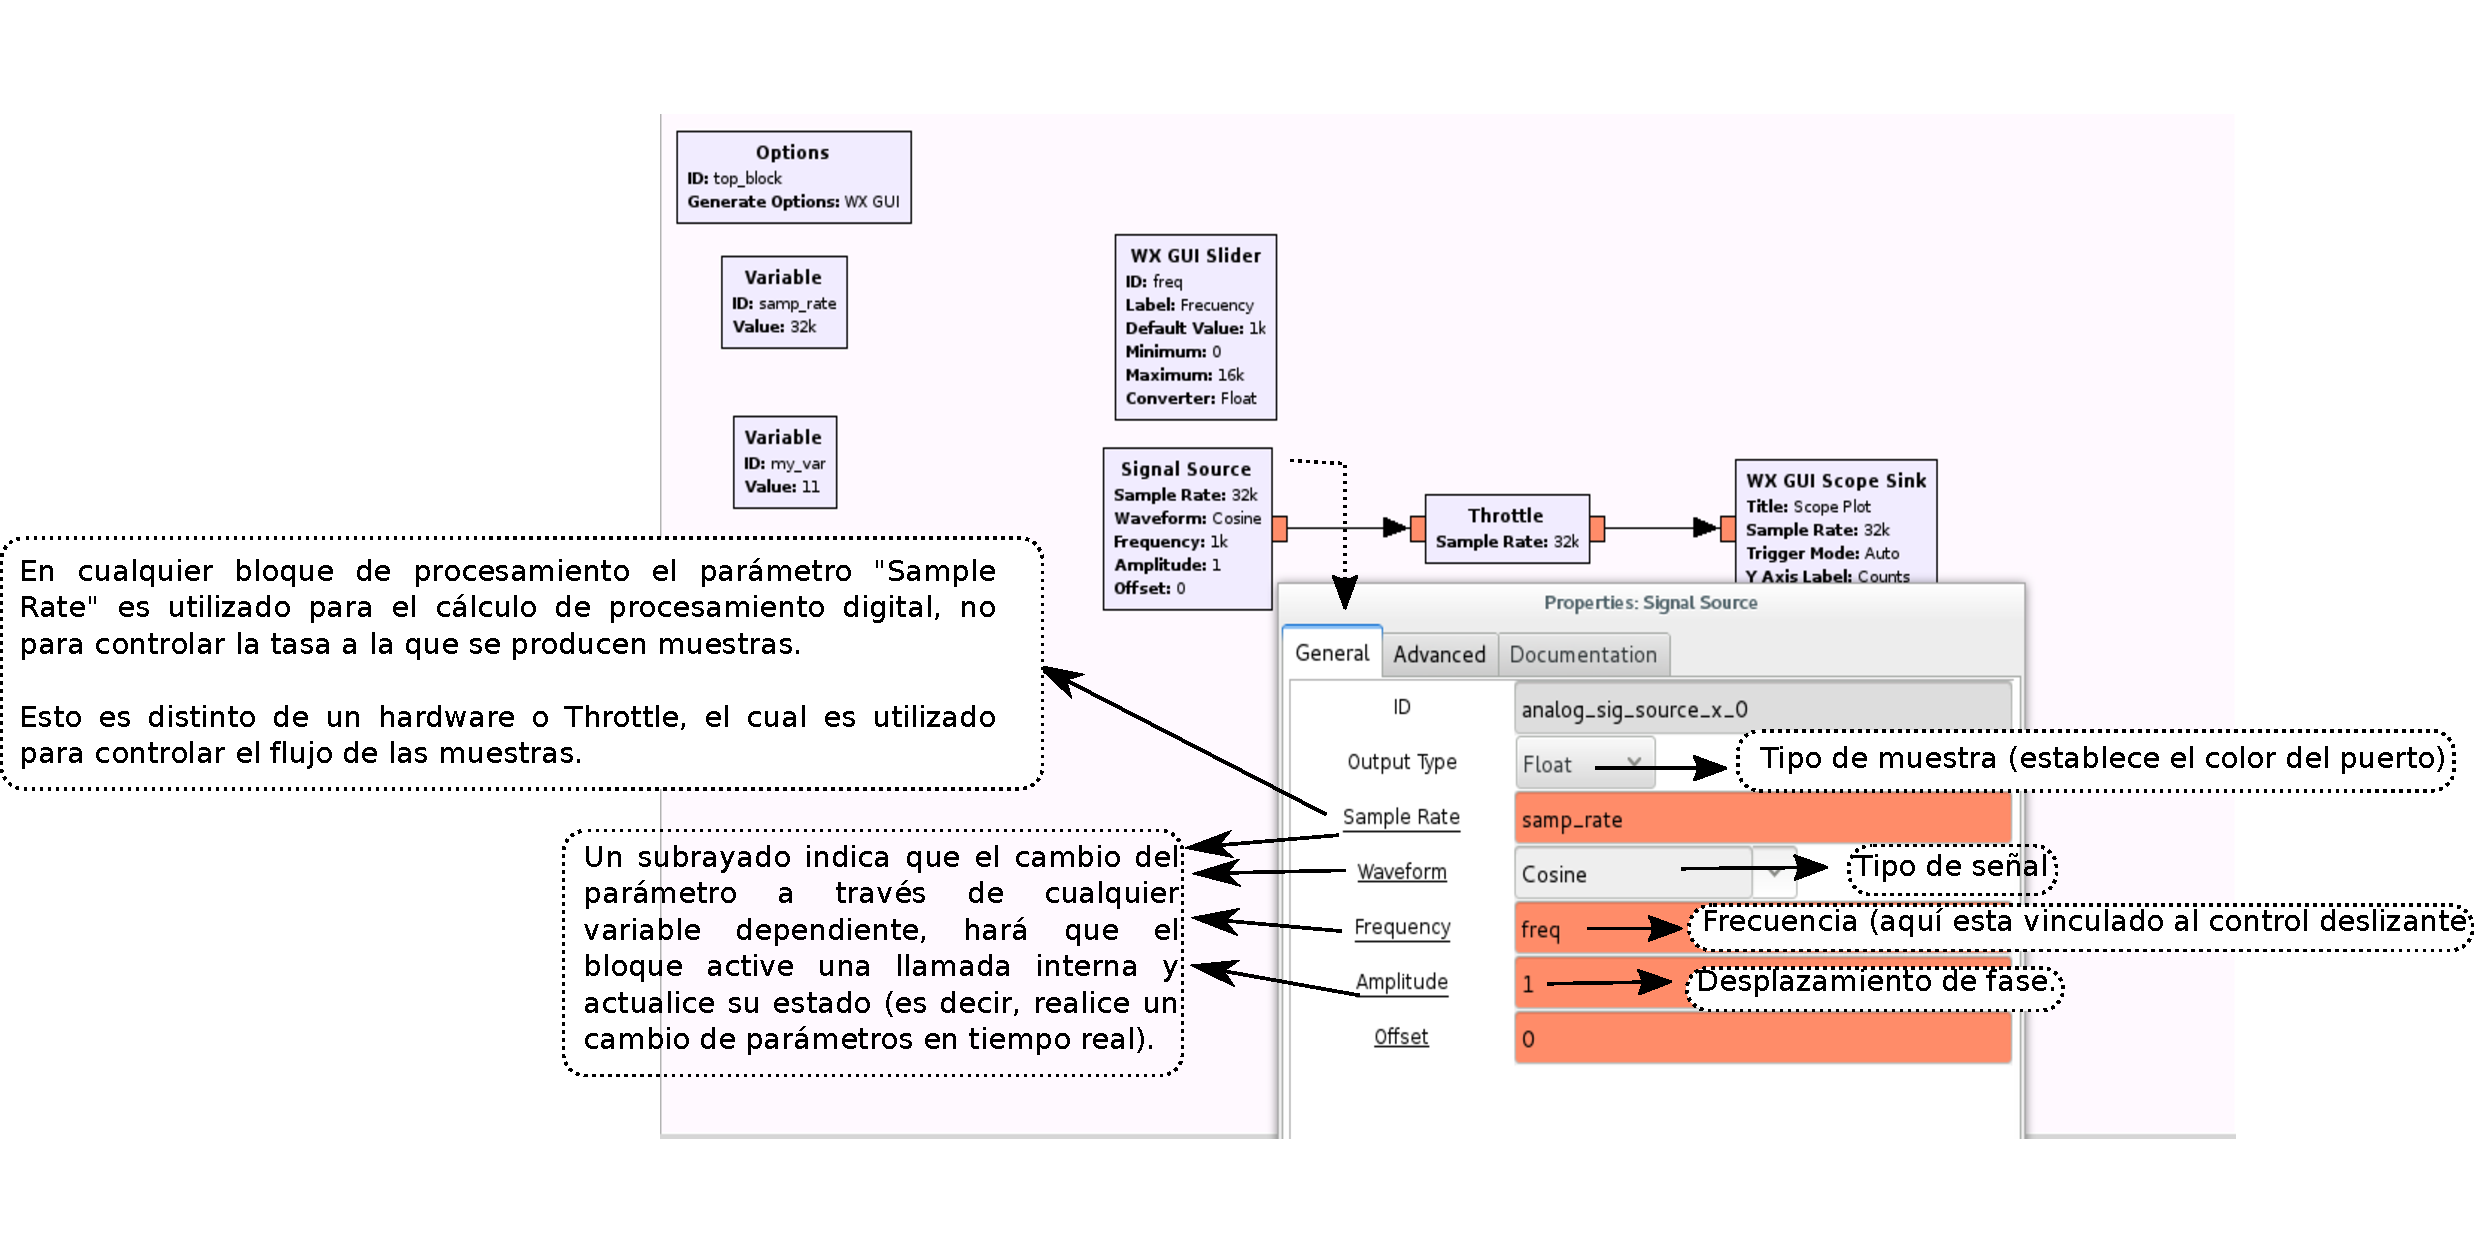
\includegraphics[width=1.05\textwidth]{parte1/lab1/pdf/lab1_14.pdf}
\end{figure}
\end{frame}
%-----------------------------------

\begin{frame}{Primeros pasos }
\begin{figure}[H]
\vspace{-3mm}
\centering
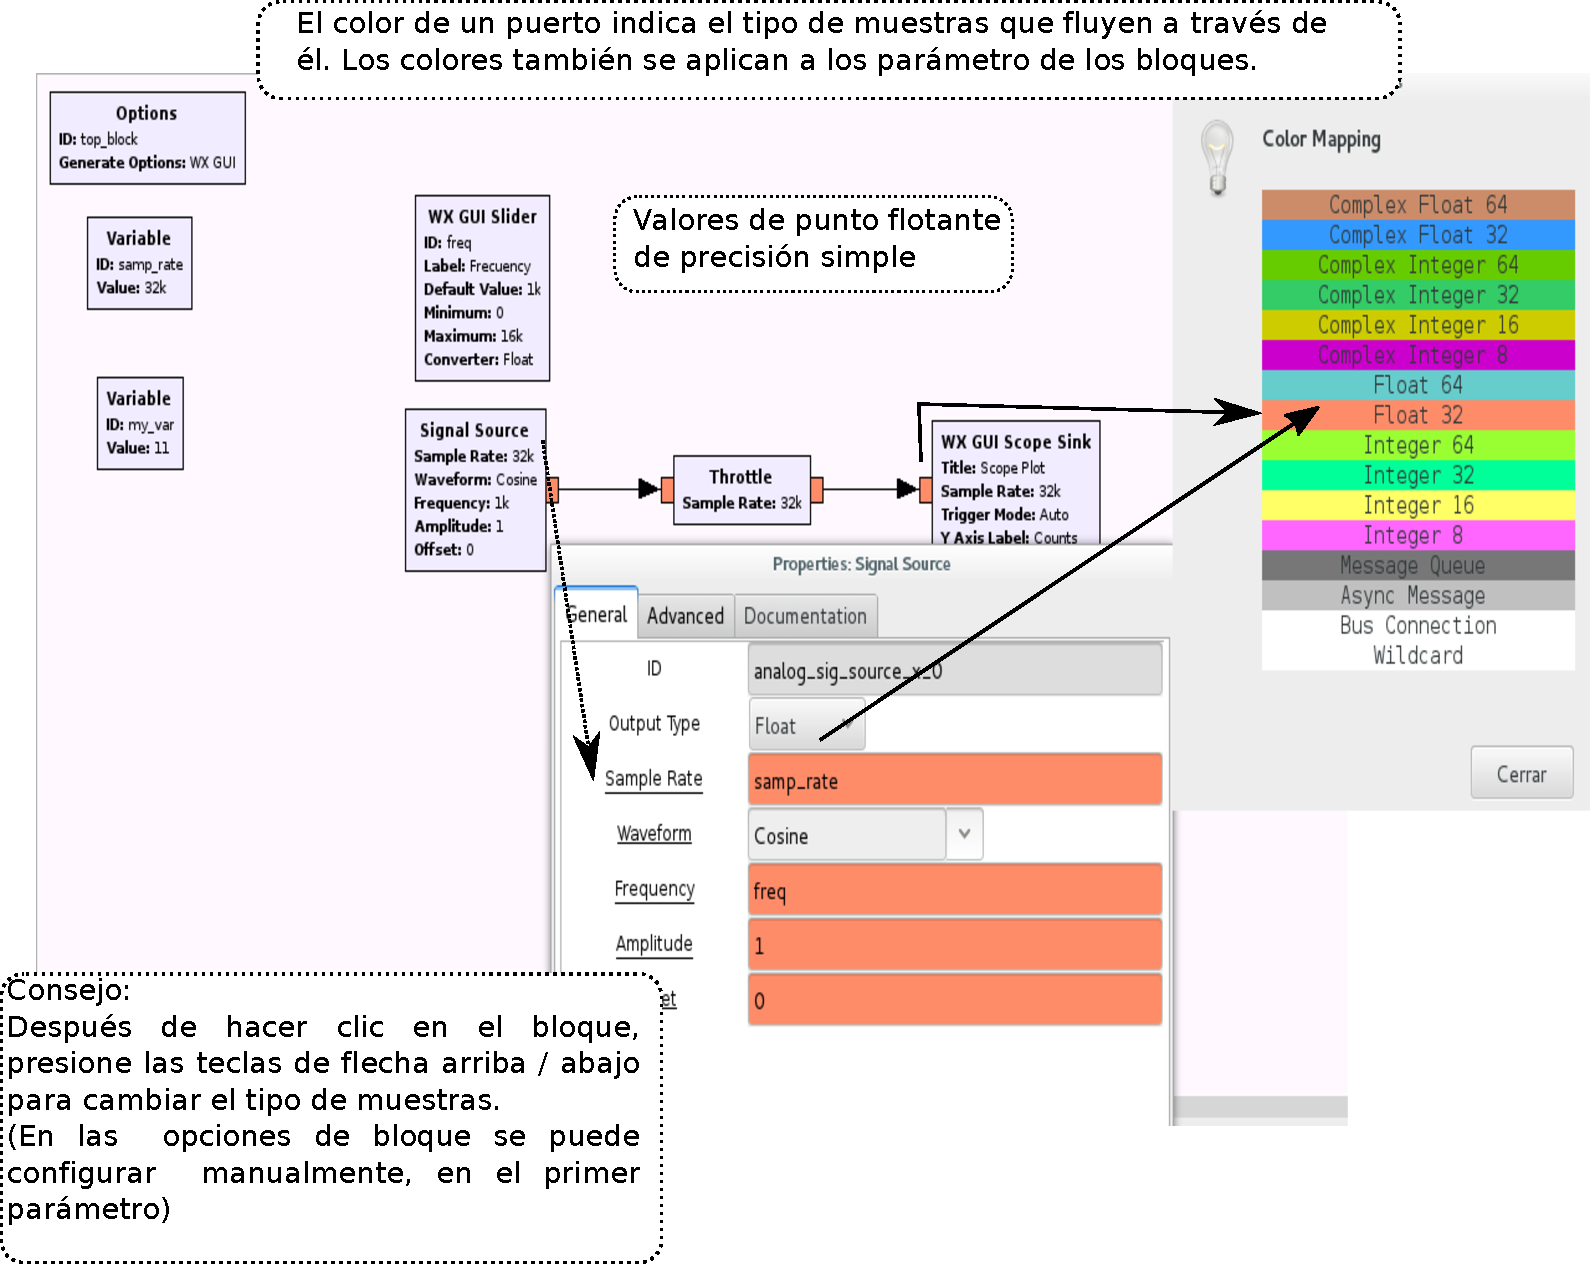
\includegraphics[width=.80\textwidth]{parte1/lab1/pdf/lab1_15.pdf}
\end{figure}
\end{frame}
%-----------------------------------

\begin{frame}{Primeros pasos }
\begin{figure}[H]
\centering
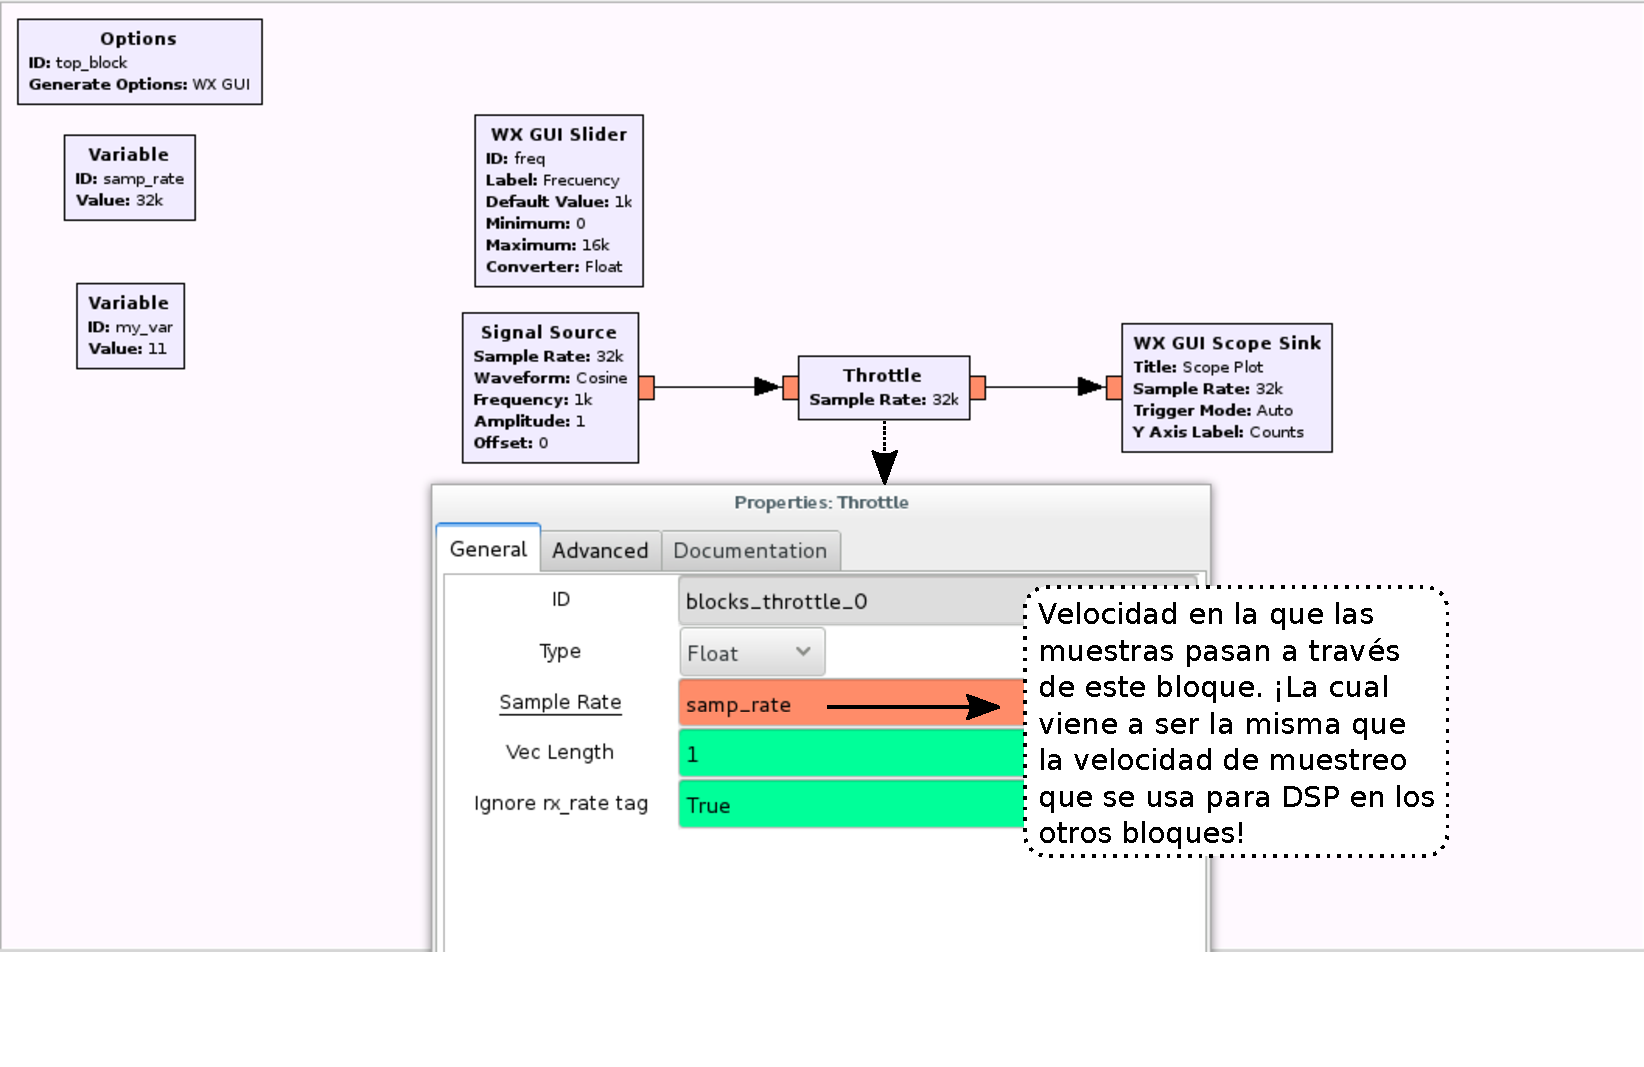
\includegraphics[width=\textwidth]{parte1/lab1/pdf/lab1_16.pdf}
\end{figure}
\end{frame}
%-----------------------------------

\begin{frame}{Primeros pasos }
\begin{figure}[H]
\vspace{-3mm}
\centering
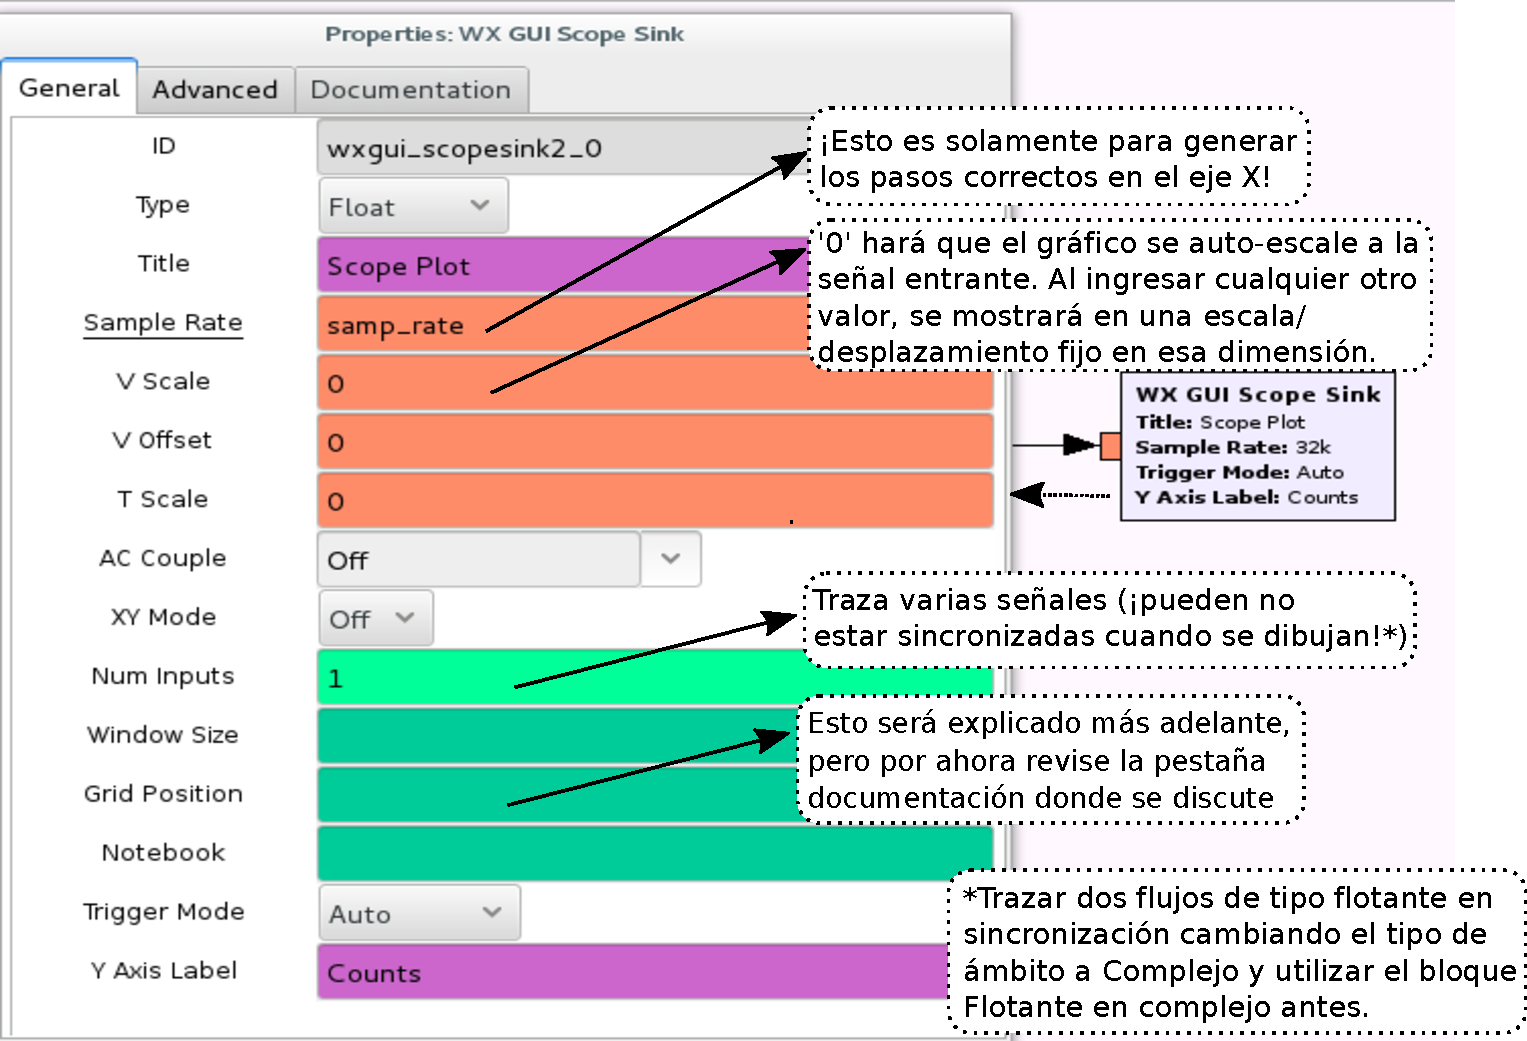
\includegraphics[width=.85\textwidth]{parte1/lab1/pdf/lab1_17.pdf}
\end{figure}
\end{frame}
%-----------------------------------

\begin{frame}{Primeros pasos }
\begin{figure}[H]
\centering
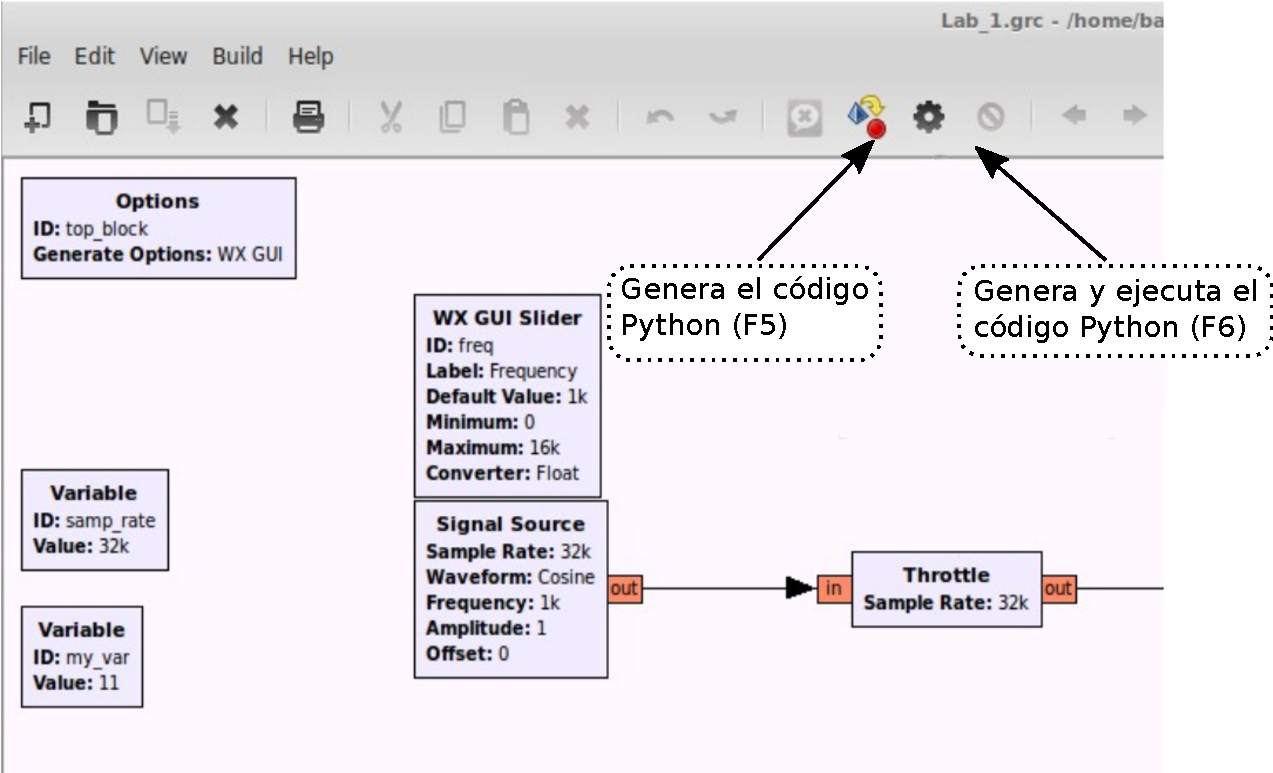
\includegraphics[width=\textwidth]{parte1/lab1/pdf/lab1_18.pdf}
\end{figure}
\end{frame}
%-----------------------------------

\begin{frame}{Primeros pasos }
\begin{figure}[H]
\centering
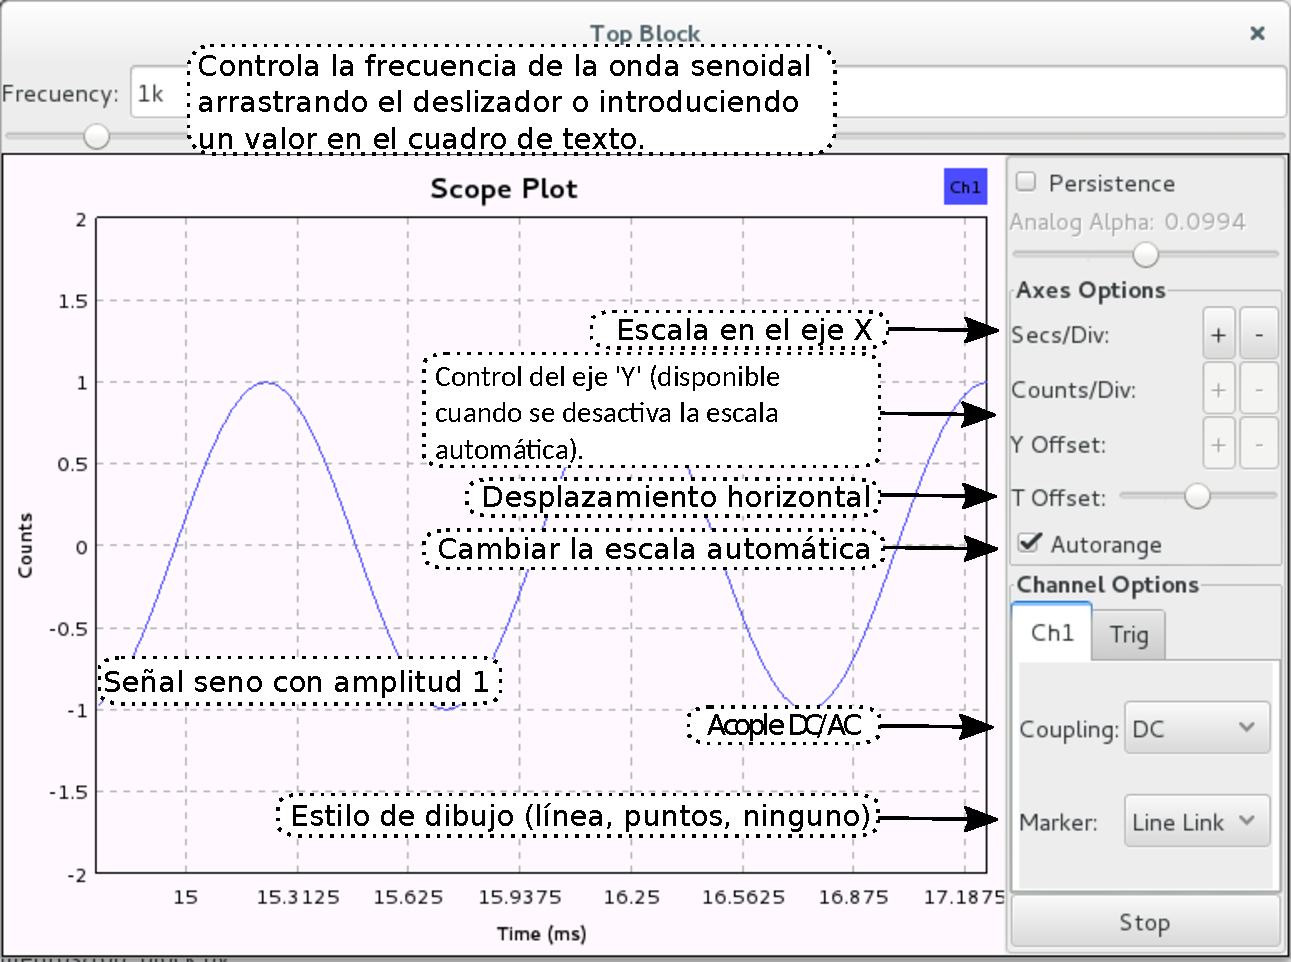
\includegraphics[width=\textwidth, height=0.55\textwidth]{parte1/lab1/pdf/lab1_19.pdf}
\end{figure}
\end{frame}
%-----------------------------------

\begin{frame}{Primeros pasos }
\begin{figure}[H]
\centering
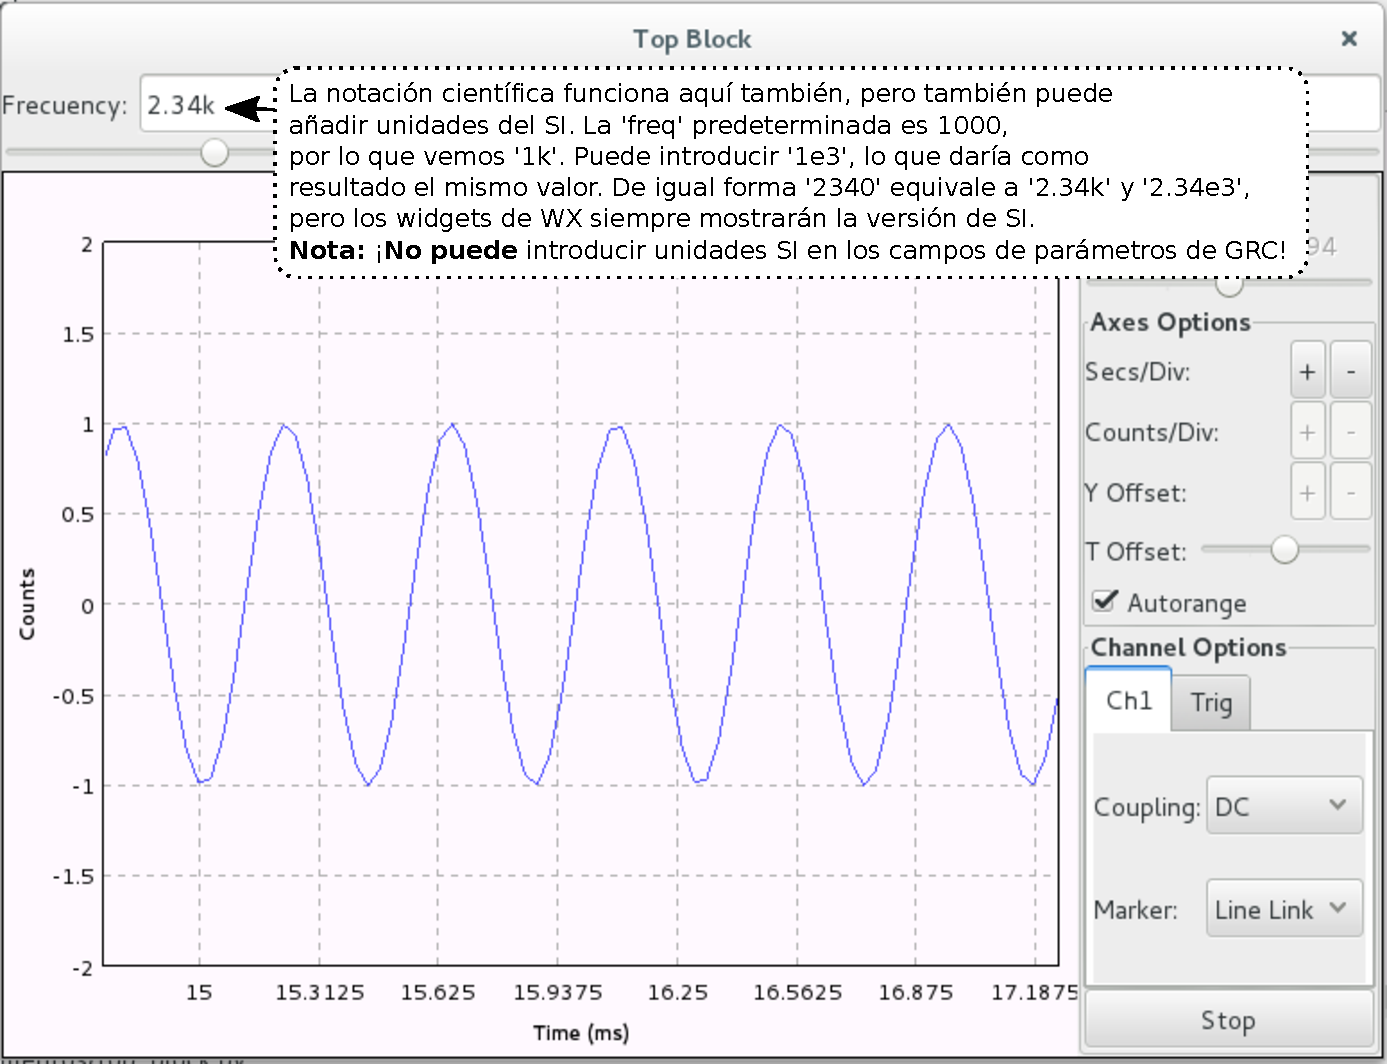
\includegraphics[width=\textwidth, height=0.55\textwidth]{parte1/lab1/pdf/lab1_20.pdf}
\end{figure}
\end{frame}
%-----------------------------------

\begin{frame}{Primeros pasos }
\begin{figure}[H]
\centering
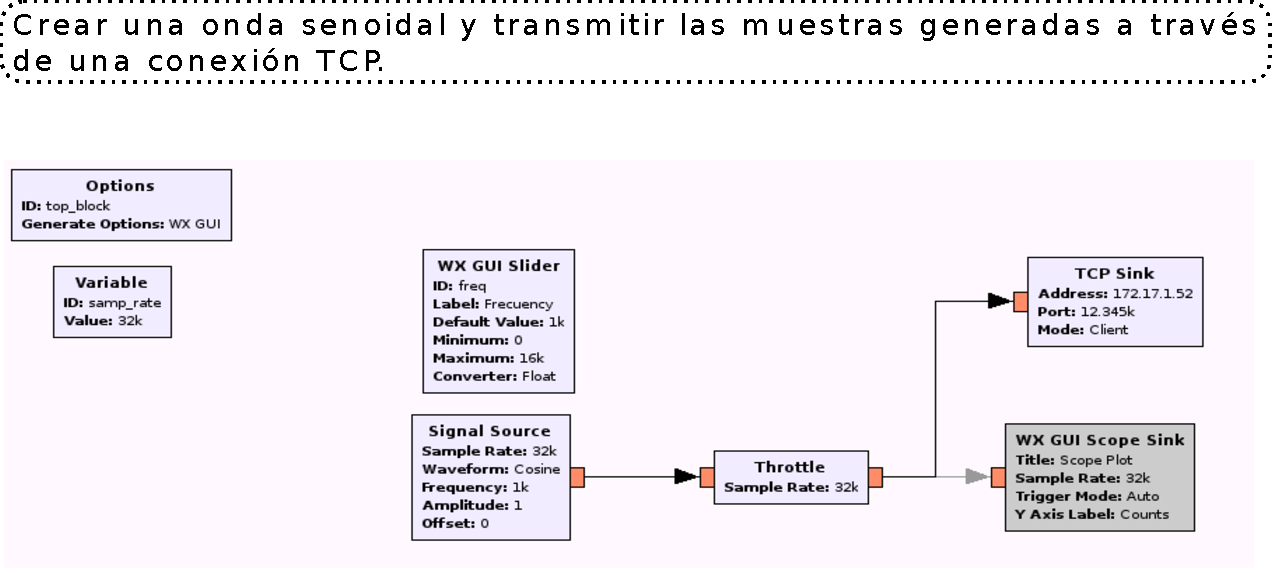
\includegraphics[width=\textwidth]{parte1/lab1/pdf/lab1_21.pdf}
\end{figure}
\end{frame}
%-----------------------------------

\begin{frame}{Primeros pasos }
\begin{figure}[H]
\centering
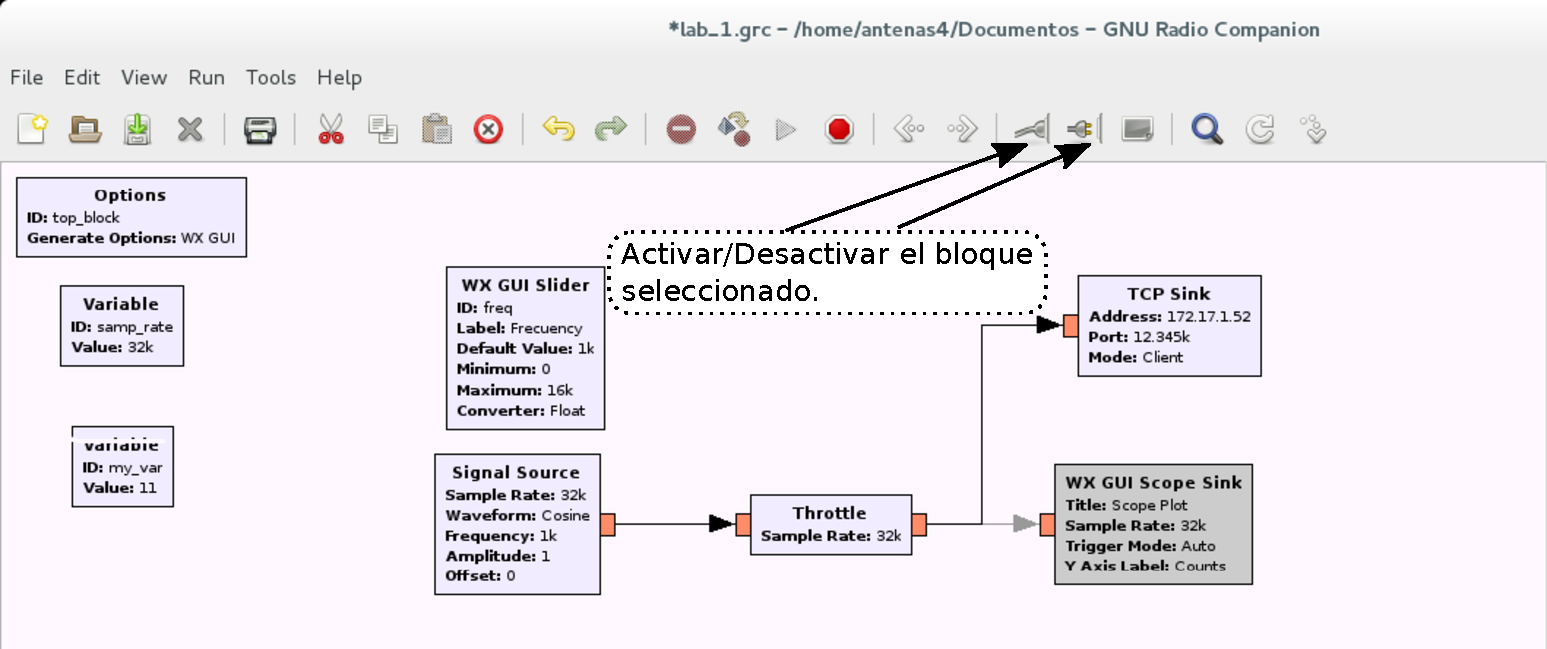
\includegraphics[width=\textwidth]{parte1/lab1/pdf/lab1_22.pdf}
\end{figure}
\end{frame}
%-----------------------------------

\begin{frame}{Primeros pasos }
\begin{figure}[H]
\centering
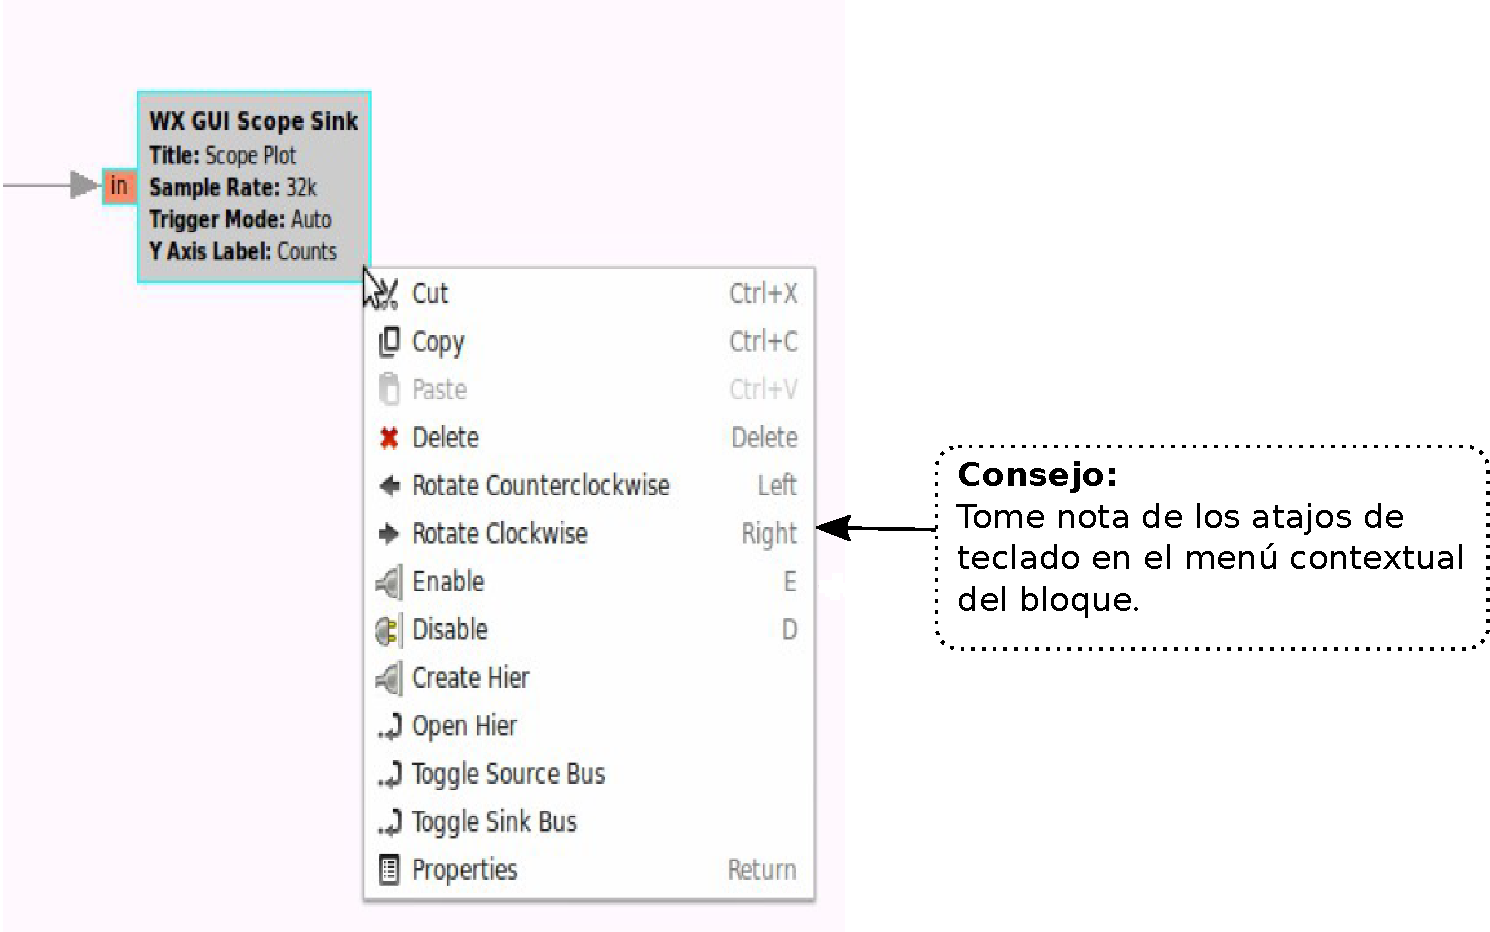
\includegraphics[width=\textwidth, height=0.6\textwidth]{parte1/lab1/pdf/lab1_23.pdf}
\end{figure}
\end{frame}
%-----------------------------------

\begin{frame}{Primeros pasos }
\begin{figure}[H]
\centering
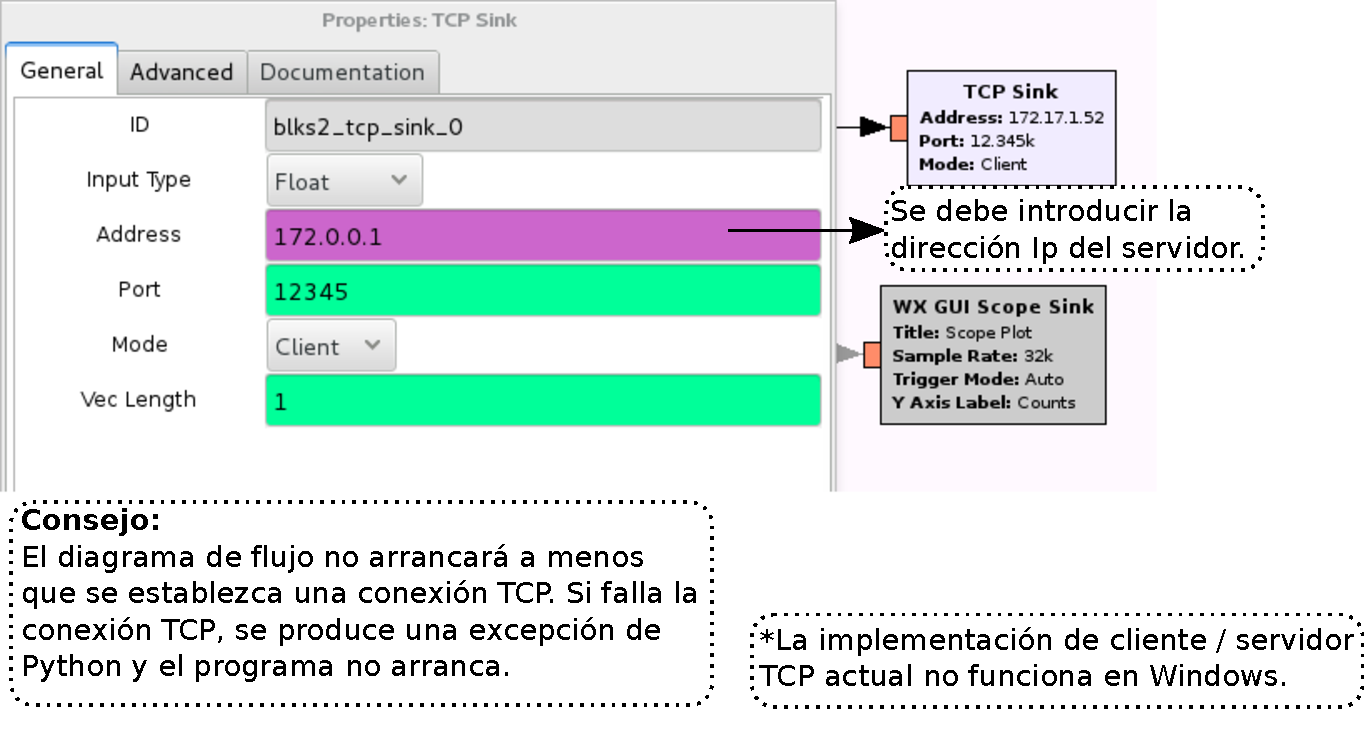
\includegraphics[width=\textwidth]{parte1/lab1/pdf/lab1_24.pdf}
\end{figure}
\end{frame}
%-----------------------------------

\begin{frame}{Primeros pasos }
\begin{figure}[H]
\centering
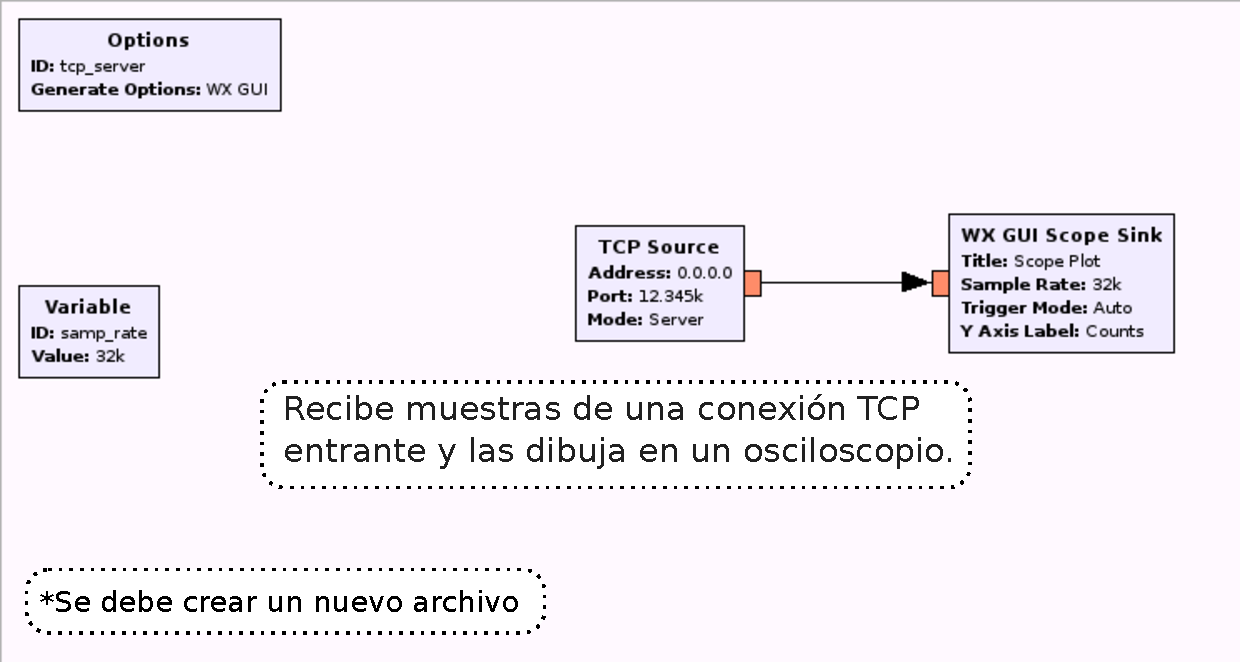
\includegraphics[width=\textwidth]{parte1/lab1/pdf/lab1_25.pdf}
\end{figure}
\end{frame}
%-----------------------------------

\begin{frame}{Primeros pasos }
\begin{figure}[H]
\centering
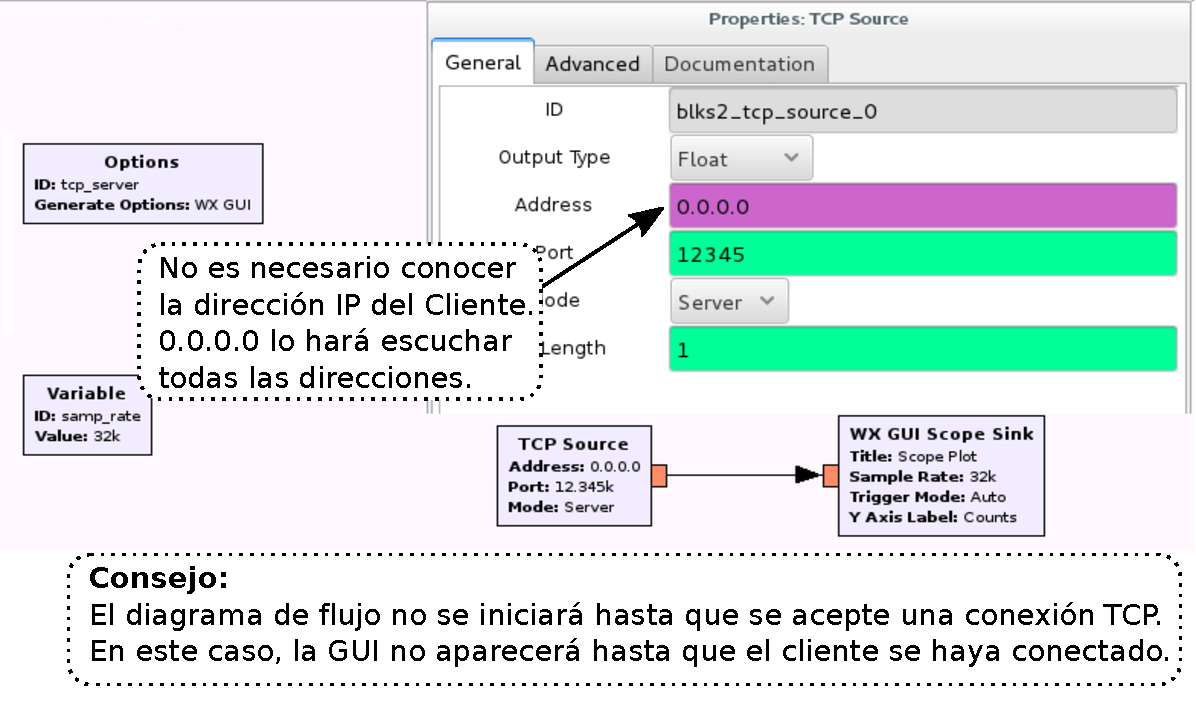
\includegraphics[width=\textwidth]{parte1/lab1/pdf/lab1_26.pdf}
\end{figure}
\end{frame}
%-----------------------------------

\begin{frame}{Primeros pasos }
\begin{figure}[H]
\centering
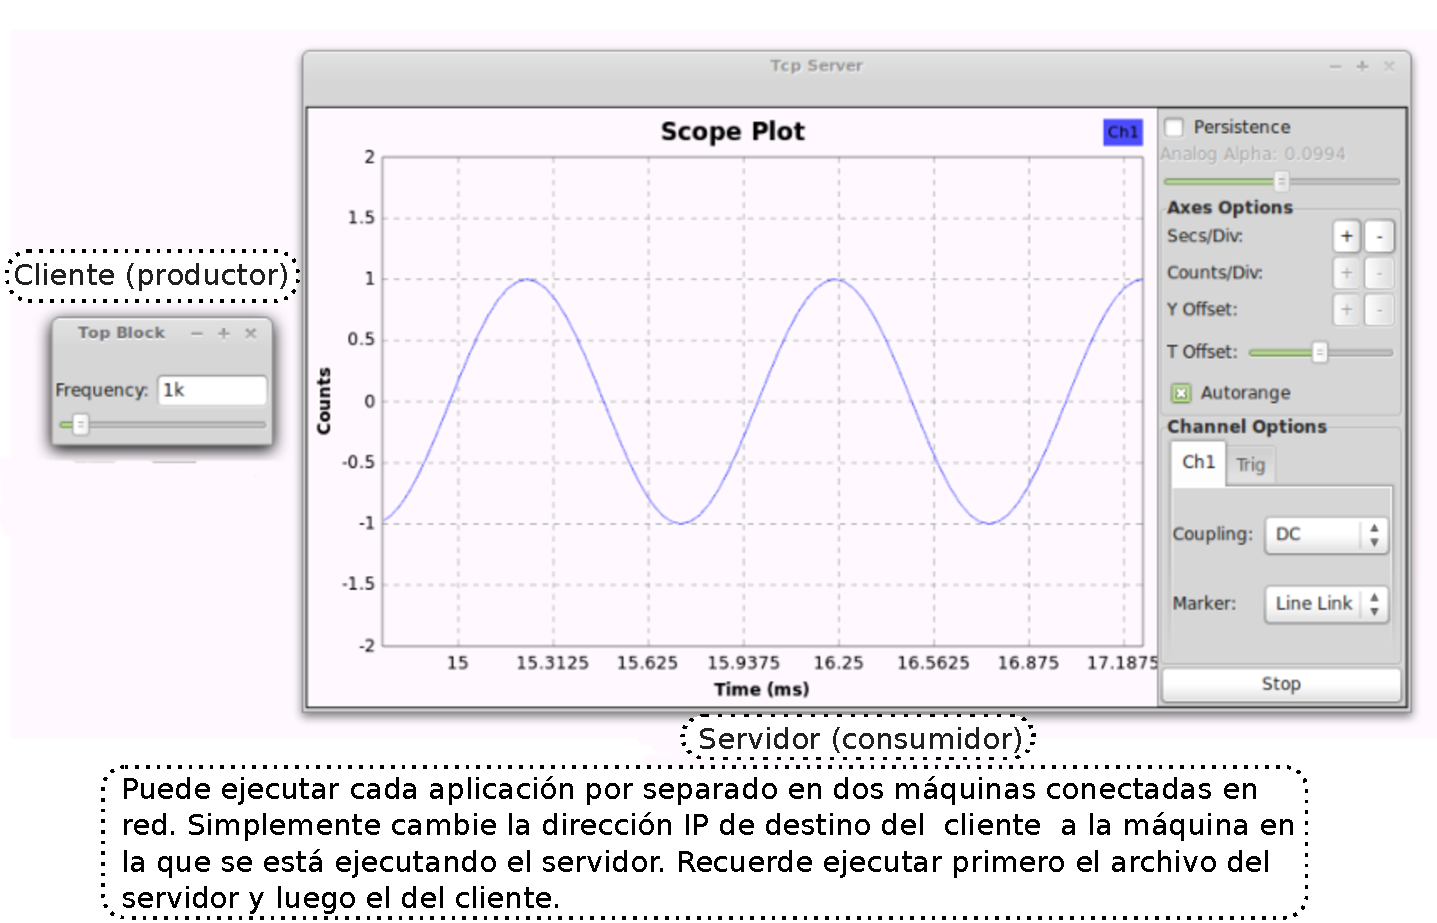
\includegraphics[width=\textwidth, height=0.55\textwidth]{parte1/lab1/pdf/lab1_27.pdf}
\end{figure}
\end{frame}
%-----------------------------------

%///////////////////////////////////////////////////////////////

\subsection{Lab2: Osciloscopio y FFT}
%*********************
\begin{frame}{}

\pgfdeclareimage[width=\paperwidth,height=\paperheight]{bg}{imagenes/fondo_lab}
\setbeamertemplate{background}{\pgfuseimage{bg}}

\bfseries{\textrm{\LARGE Lab2\\ \Large Osciloscopio y FFT}}
\raggedright
\end{frame}
%*********************

%-----------------------------------
\begin{frame}{Osciloscopio y FFT\index{TCP}}

\pgfdeclareimage[width=\paperwidth,height=\paperheight]{bg}{imagenes/fondo3}
\setbeamertemplate{background}{\pgfuseimage{bg}}

En este laboratorio se genera una onda senoidal y a su vez algún ruido; estas dos señales se suman y se observa el resultado en el dominio de la frecuencia (FFT) y del tiempo (Scope). Se aprende a utilizar el notebook y algunas herramientas básicas del GRC. 

\end{frame}
%---------------------------------

\begin{frame}{Osciloscopio y FFT\index{TCP}}

\begin{figure}[H]
\vspace{-4mm}
\centering
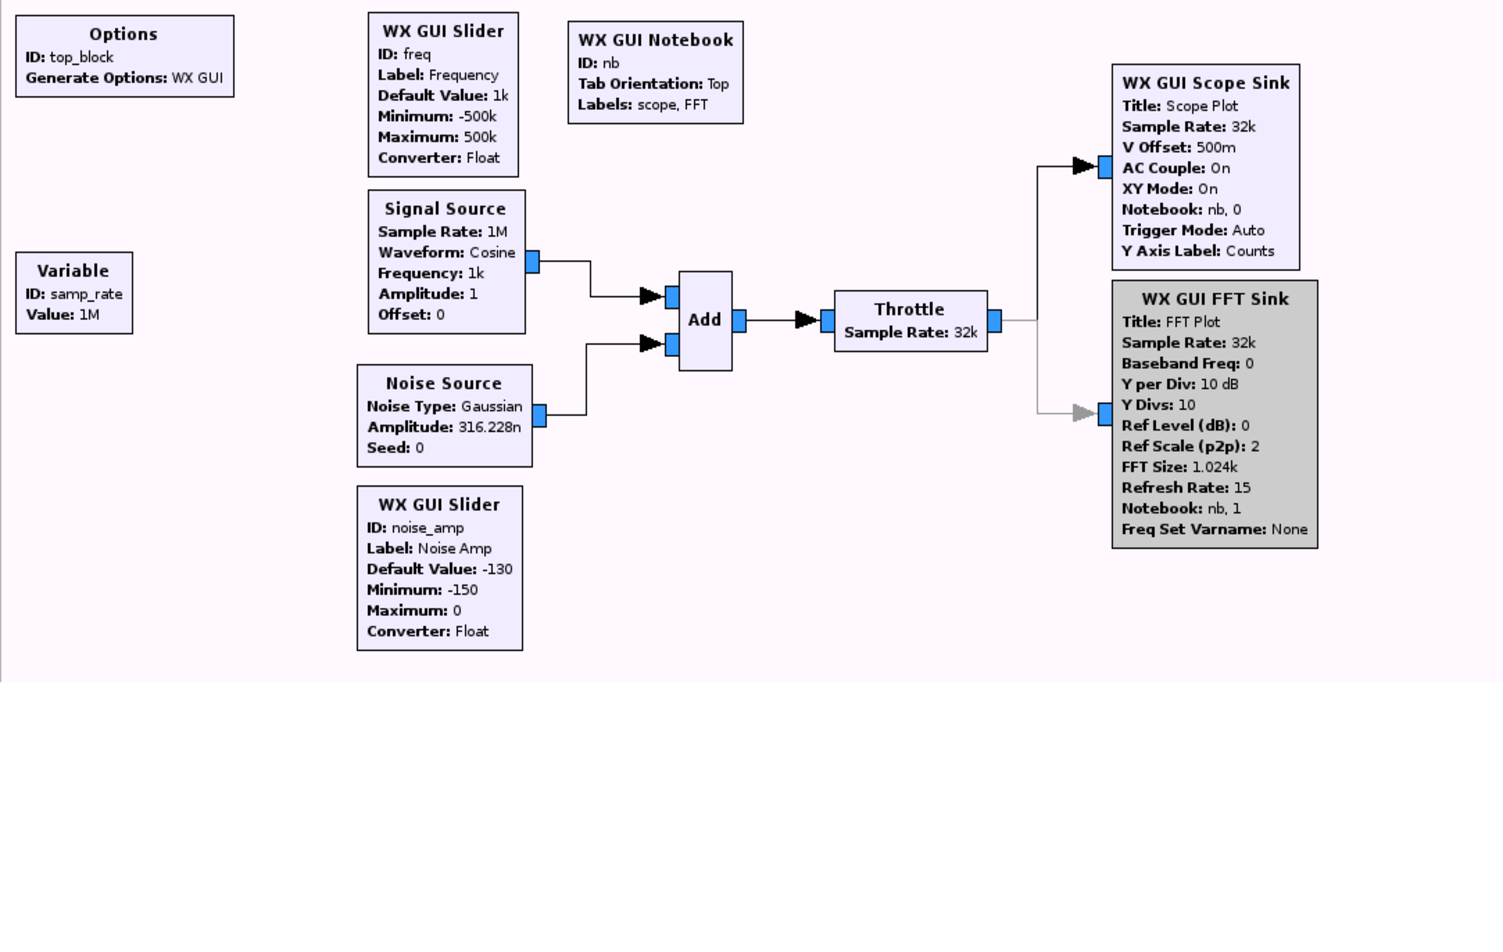
\includegraphics[width=1.2\textwidth]{parte1/lab2/pdf/lab2_1.pdf}
\end{figure}
\end{frame}
%---------------------------------

\begin{frame}{Osciloscopio y FFT}
\begin{figure}[H]
\vspace{-4mm}
\centering
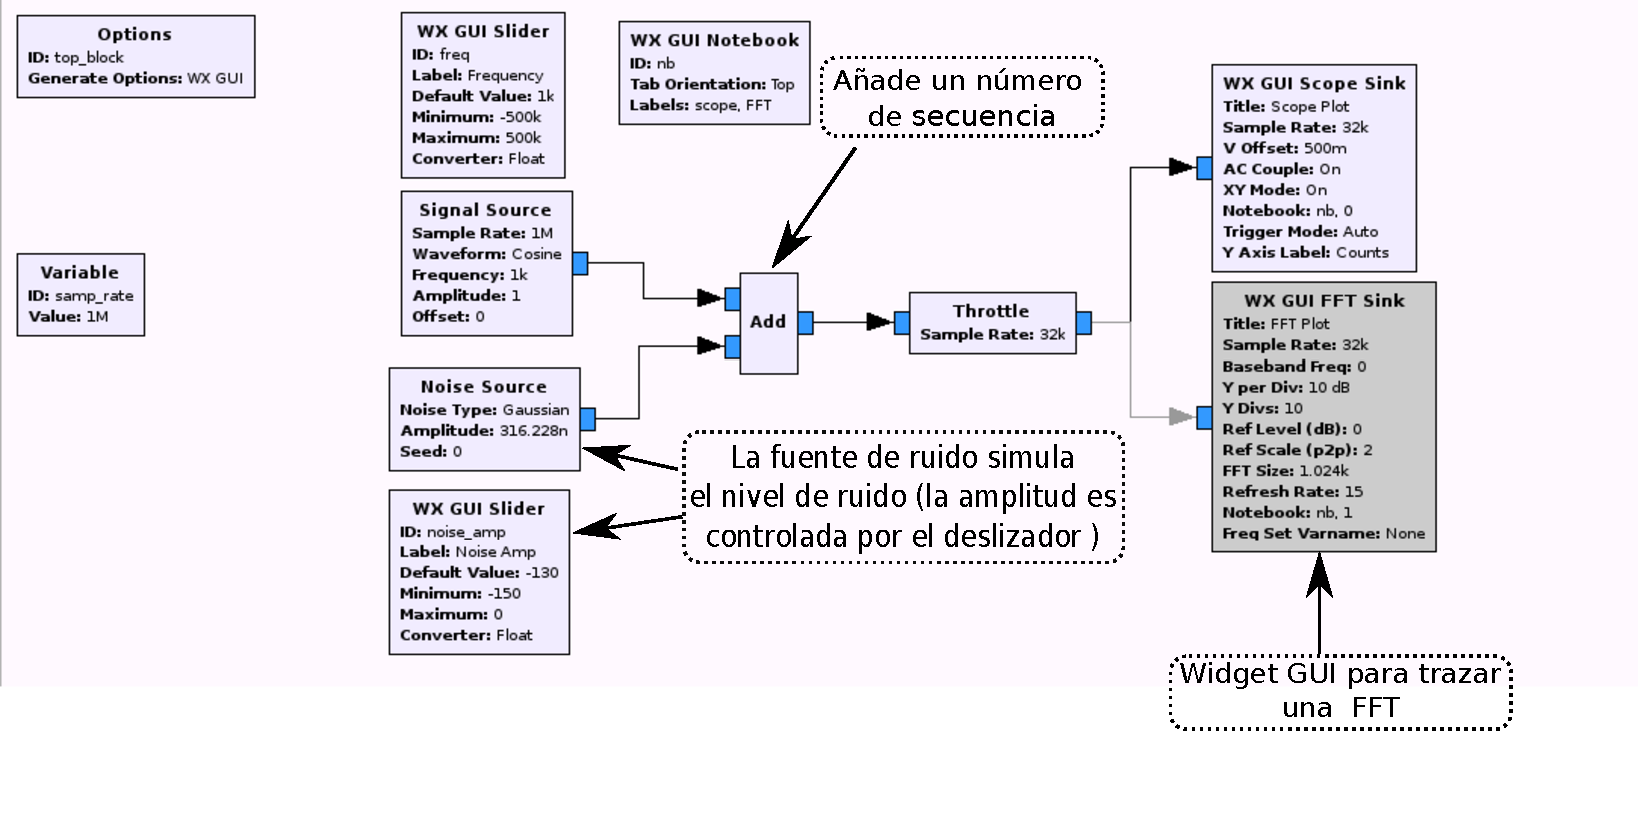
\includegraphics[width=1.1\textwidth]{parte1/lab2/pdf/lab2_2.pdf}
\end{figure}
\end{frame}
%--------------------------------

\begin{frame}{Osciloscopio y FFT\index{Noise Source}}
\begin{figure}[H]
\centering
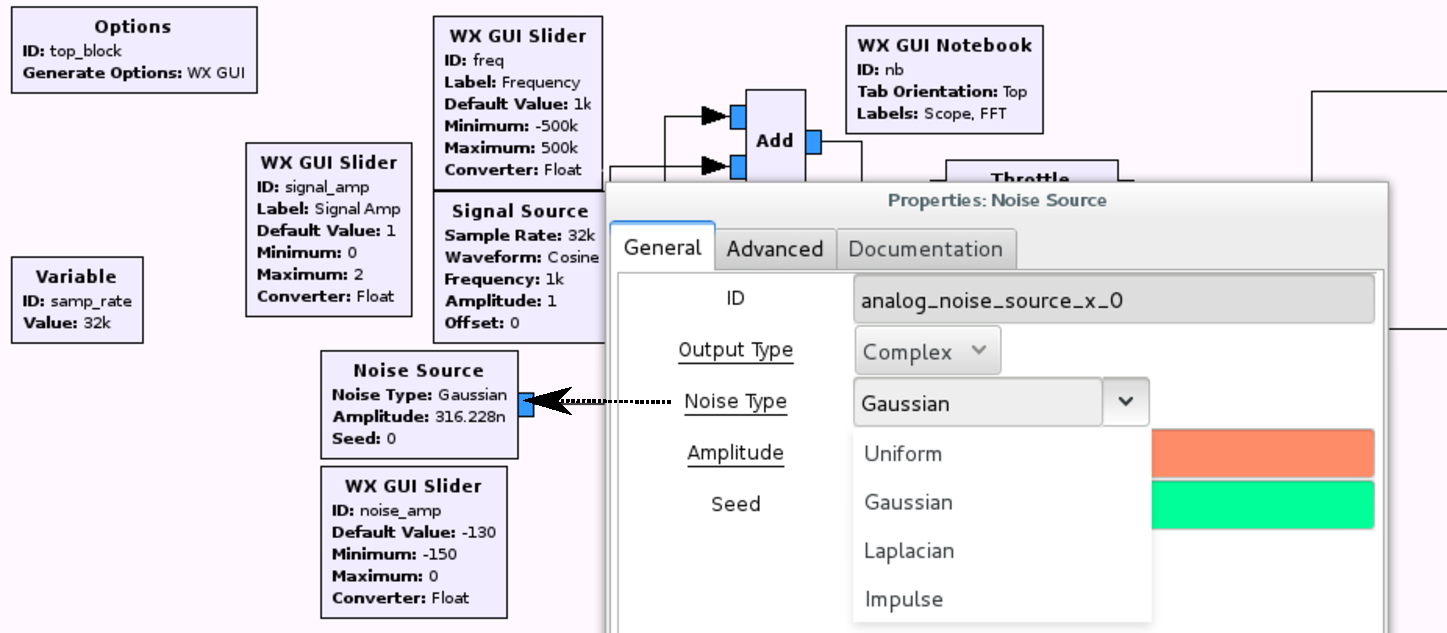
\includegraphics[width=1.055\textwidth]{parte1/lab2/pdf/lab2_3.pdf}
\end{figure}
\end{frame}
%--------------------------------

\begin{frame}{Osciloscopio y FFT\index{Noise Source}}
\begin{figure}[H]
\centering
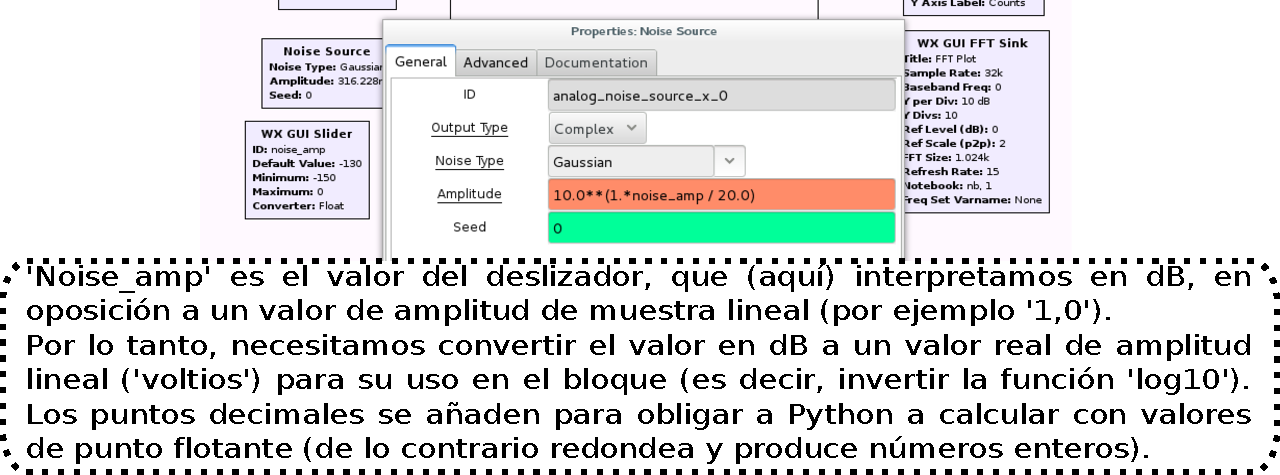
\includegraphics[width=1.055\textwidth]{parte1/lab2/pdf/lab2_4.pdf}
\end{figure}
\end{frame}
%--------------------------------

\begin{frame}{Osciloscopio y FFT\index{Add}}
\begin{figure}[H]
\centering
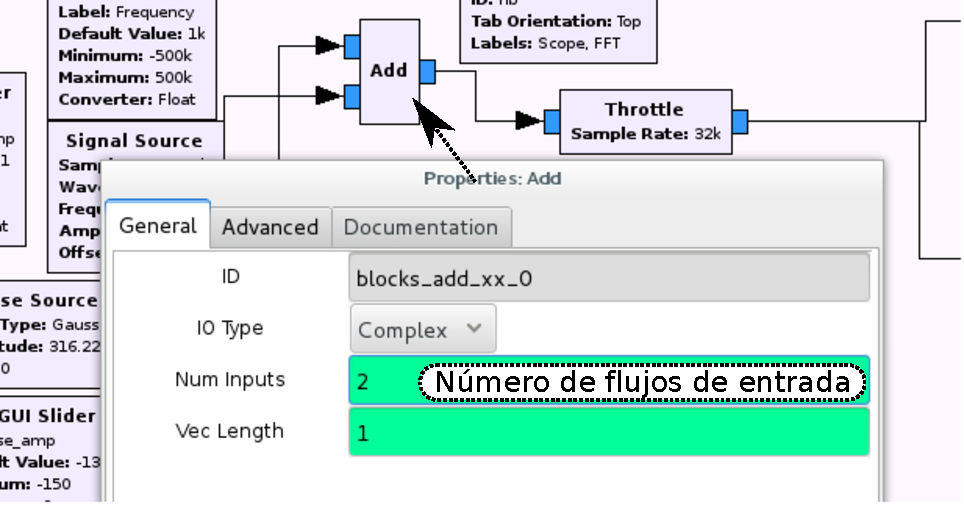
\includegraphics[width=.7\textwidth]{parte1/lab2/pdf/lab2_5.pdf}
\end{figure}
\end{frame}
%--------------------------------

\begin{frame}{Osciloscopio y FFT}
\begin{figure}[H]
\vspace{-4mm}
\centering
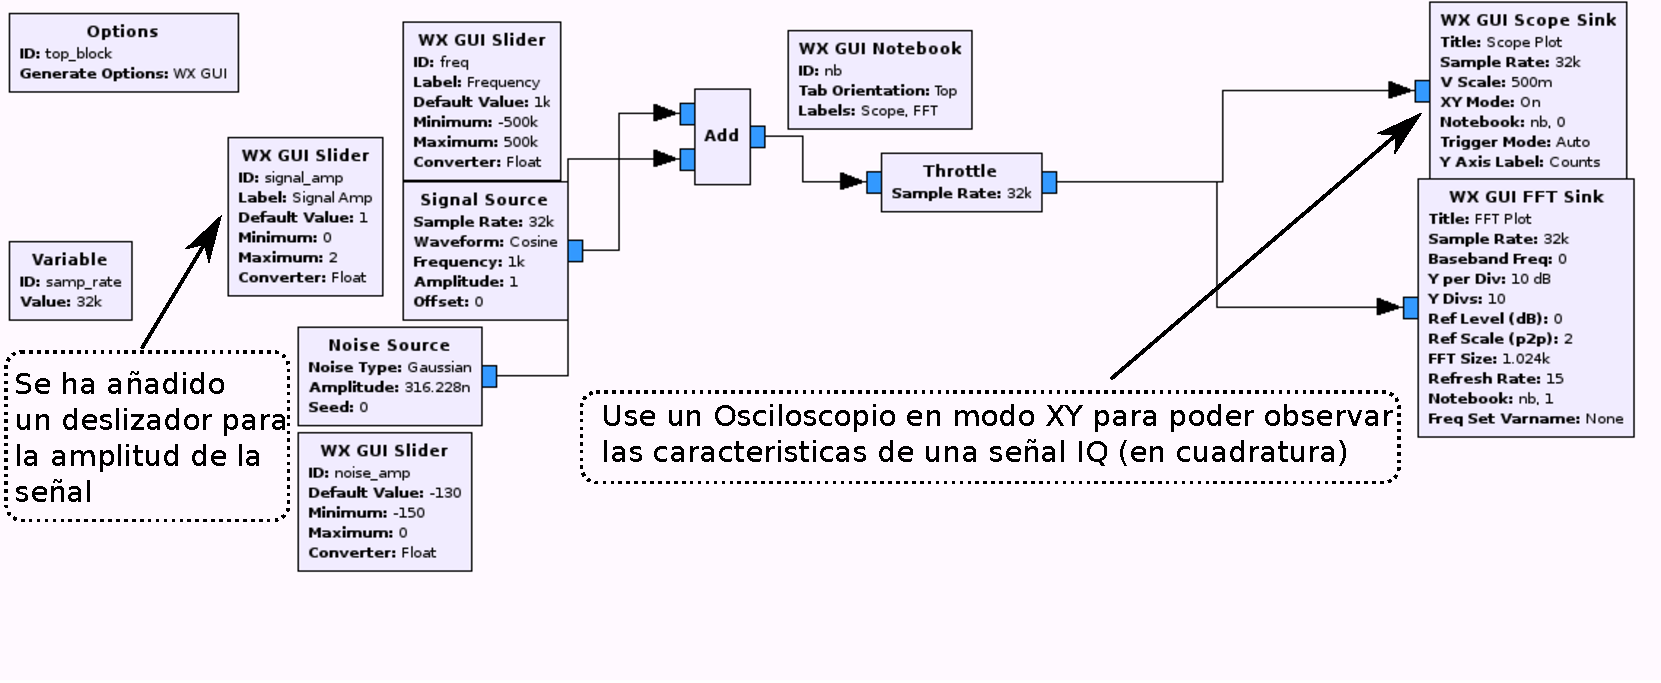
\includegraphics[width=1.1\textwidth]{parte1/lab2/pdf/lab2_6.pdf}
\end{figure}
\end{frame}
%--------------------------------

\begin{frame}{Osciloscopio y FFT\index{WX GUI Notebook}}
\begin{figure}[H]
\vspace{-4mm}
\centering
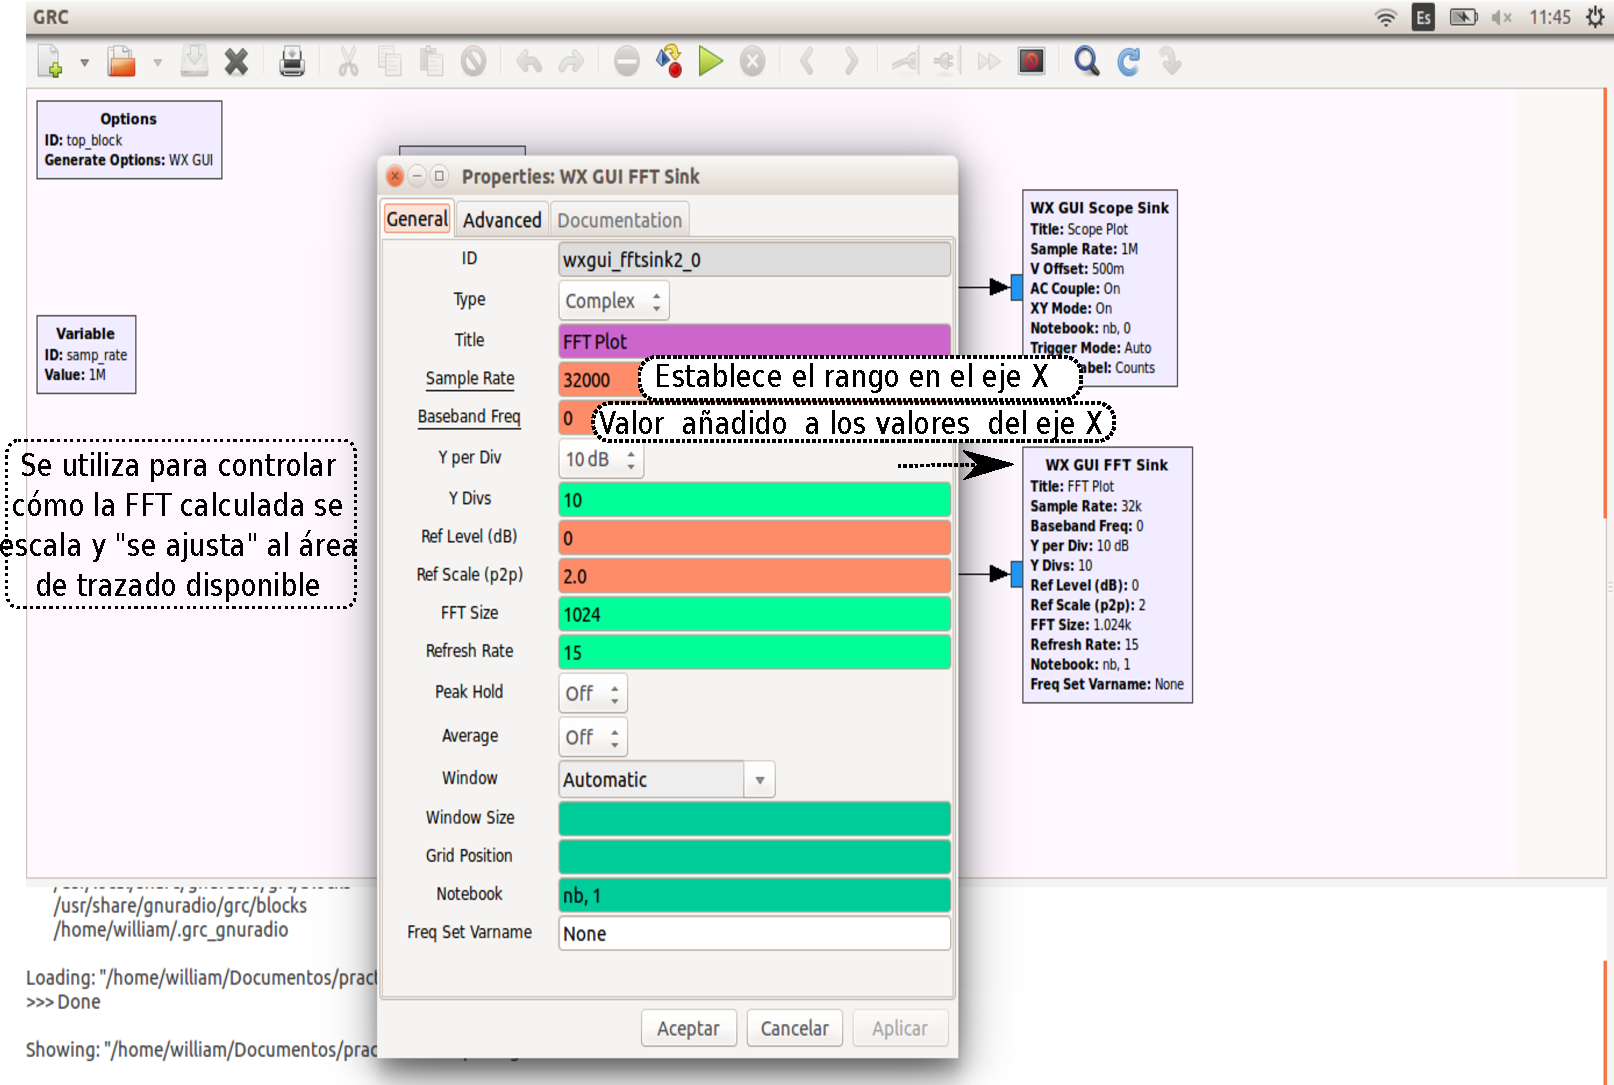
\includegraphics[width=0.85\textwidth]{parte1/lab2/pdf/lab2_7.pdf}
\end{figure}
\end{frame}
%--------------------------------

\begin{frame}{Osciloscopio y FFT\index{WX GUI FFT Sink}}
\begin{figure}[H]
\centering
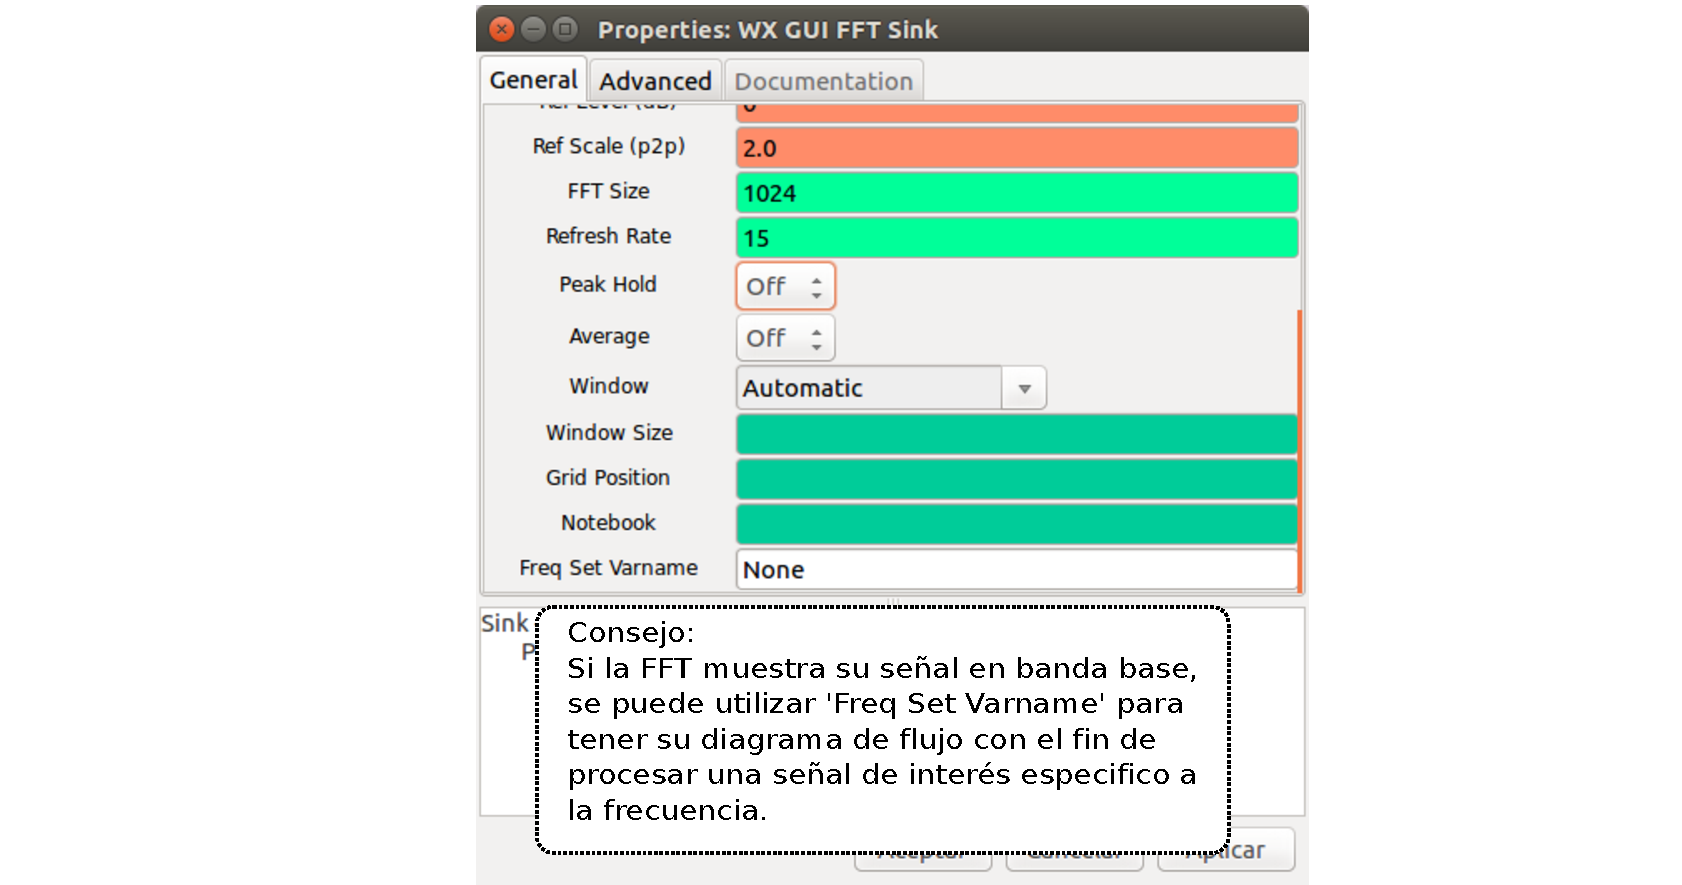
\includegraphics[width=1.1\textwidth]{parte1/lab2/pdf/lab2_8.pdf}
\end{figure}
\end{frame}
%--------------------------------

\begin{frame}{Osciloscopio y FFT\index{WX GUI FFT Sink}}
\begin{figure}[H]
\vspace{-3mm}
\centering
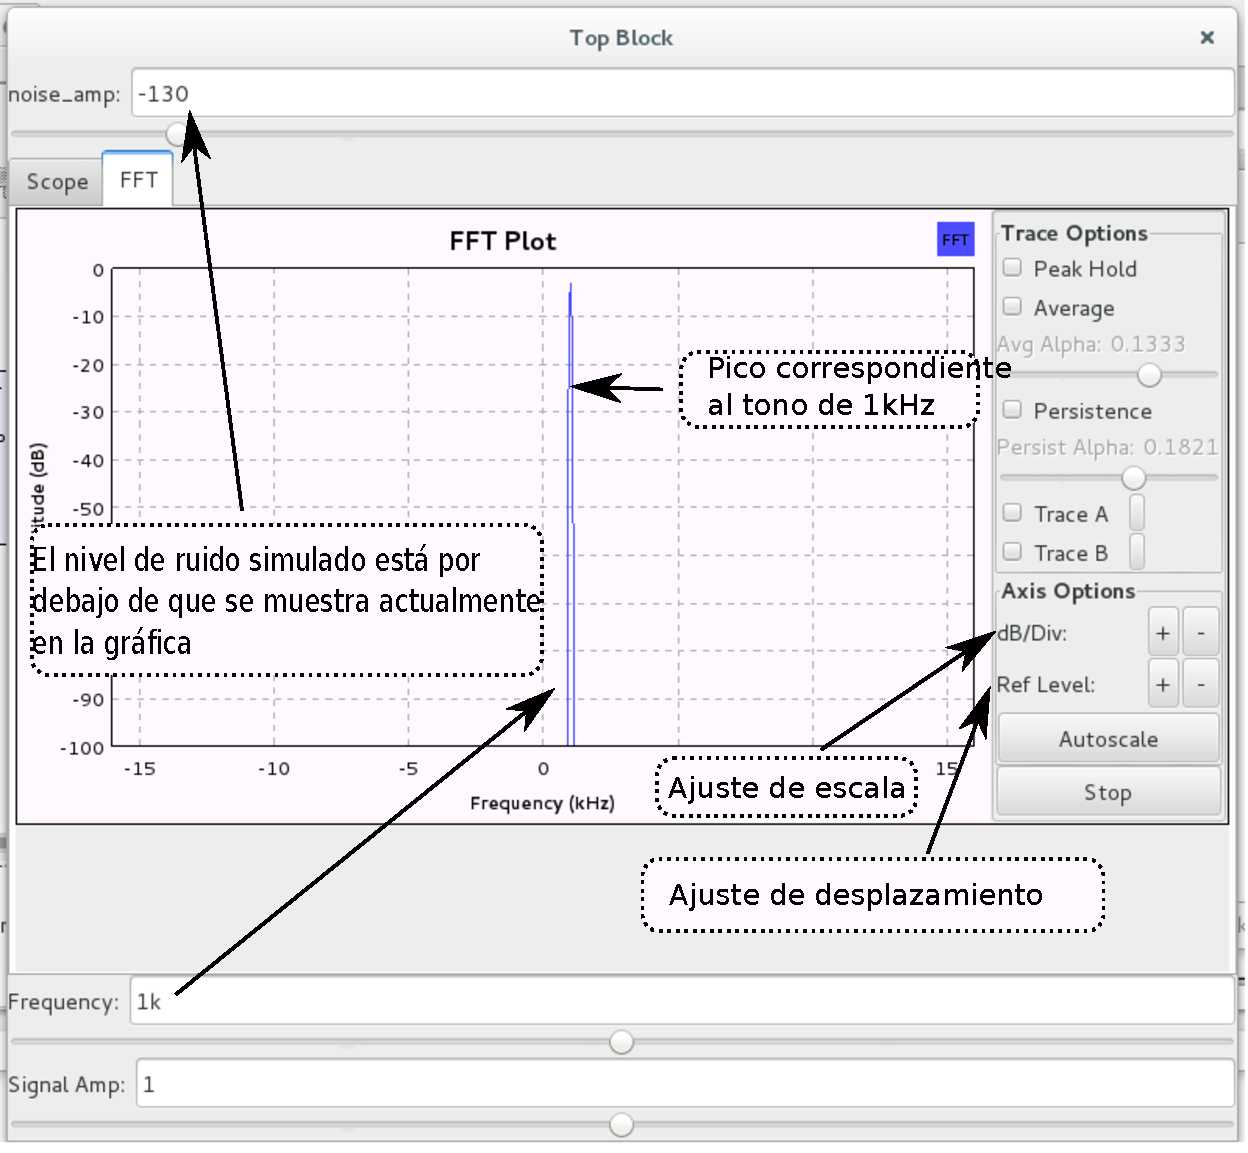
\includegraphics[width=0.7\textwidth]{parte1/lab2/pdf/lab2_9.pdf}
\end{figure}
\end{frame}
%--------------------------------

\begin{frame}{Osciloscopio y FFT}
\begin{figure}[H]
\vspace{-3mm}
\centering
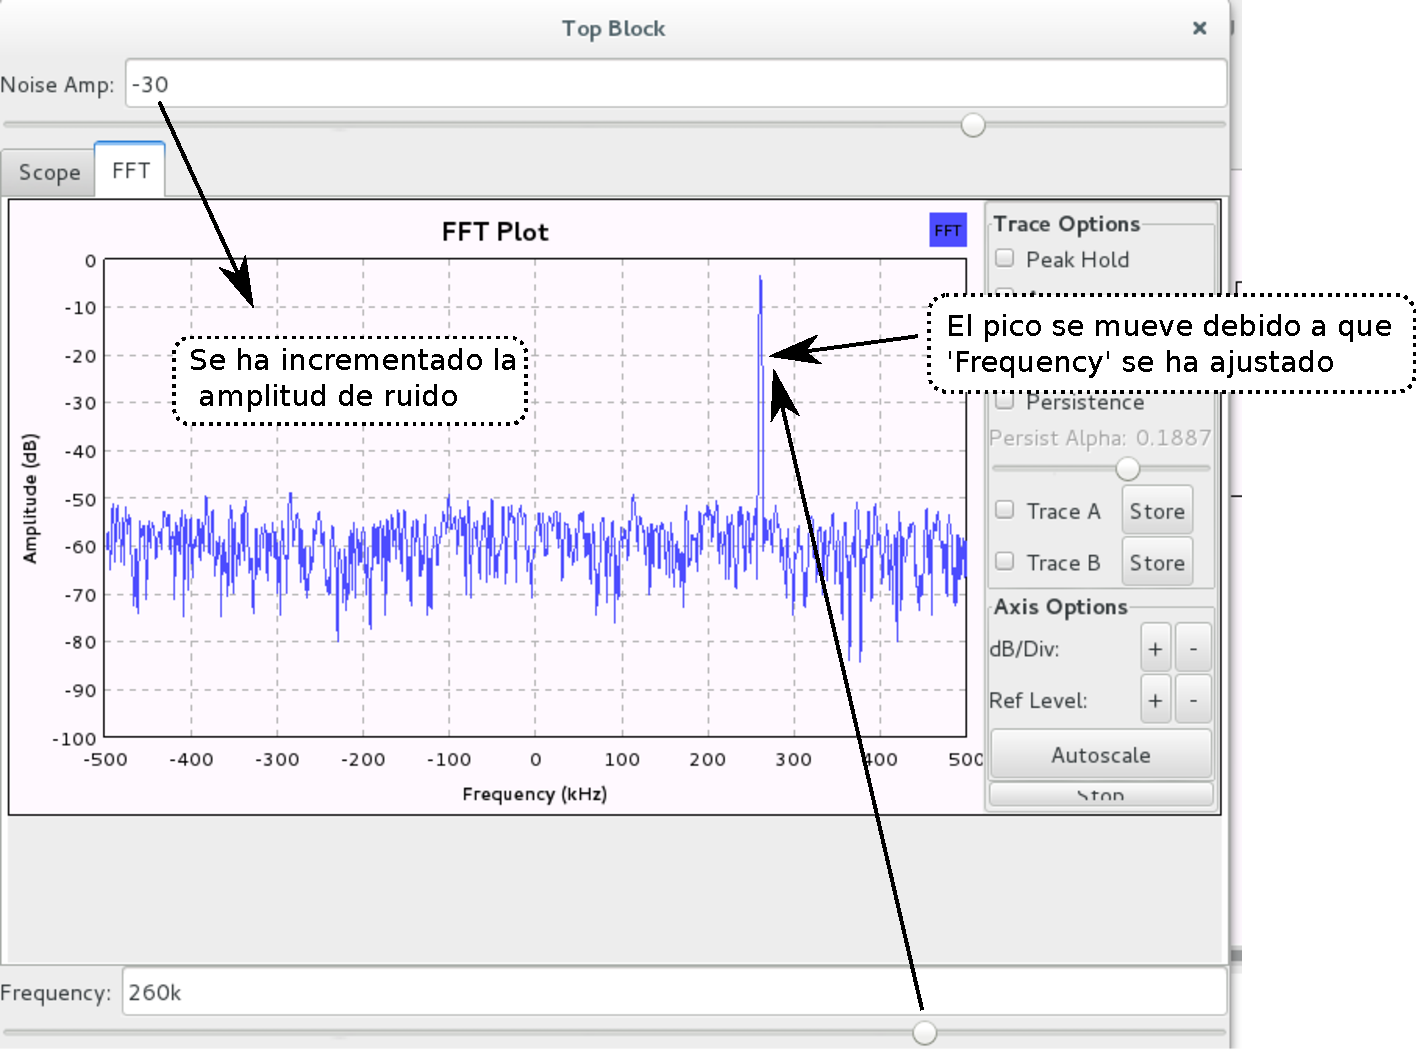
\includegraphics[width=0.85\textwidth]{parte1/lab2/pdf/lab2_10.pdf}
\end{figure}
\end{frame}
%--------------------------------

\begin{frame}{Osciloscopio y FFT}
\begin{figure}[H]
\vspace{-3mm}
\centering
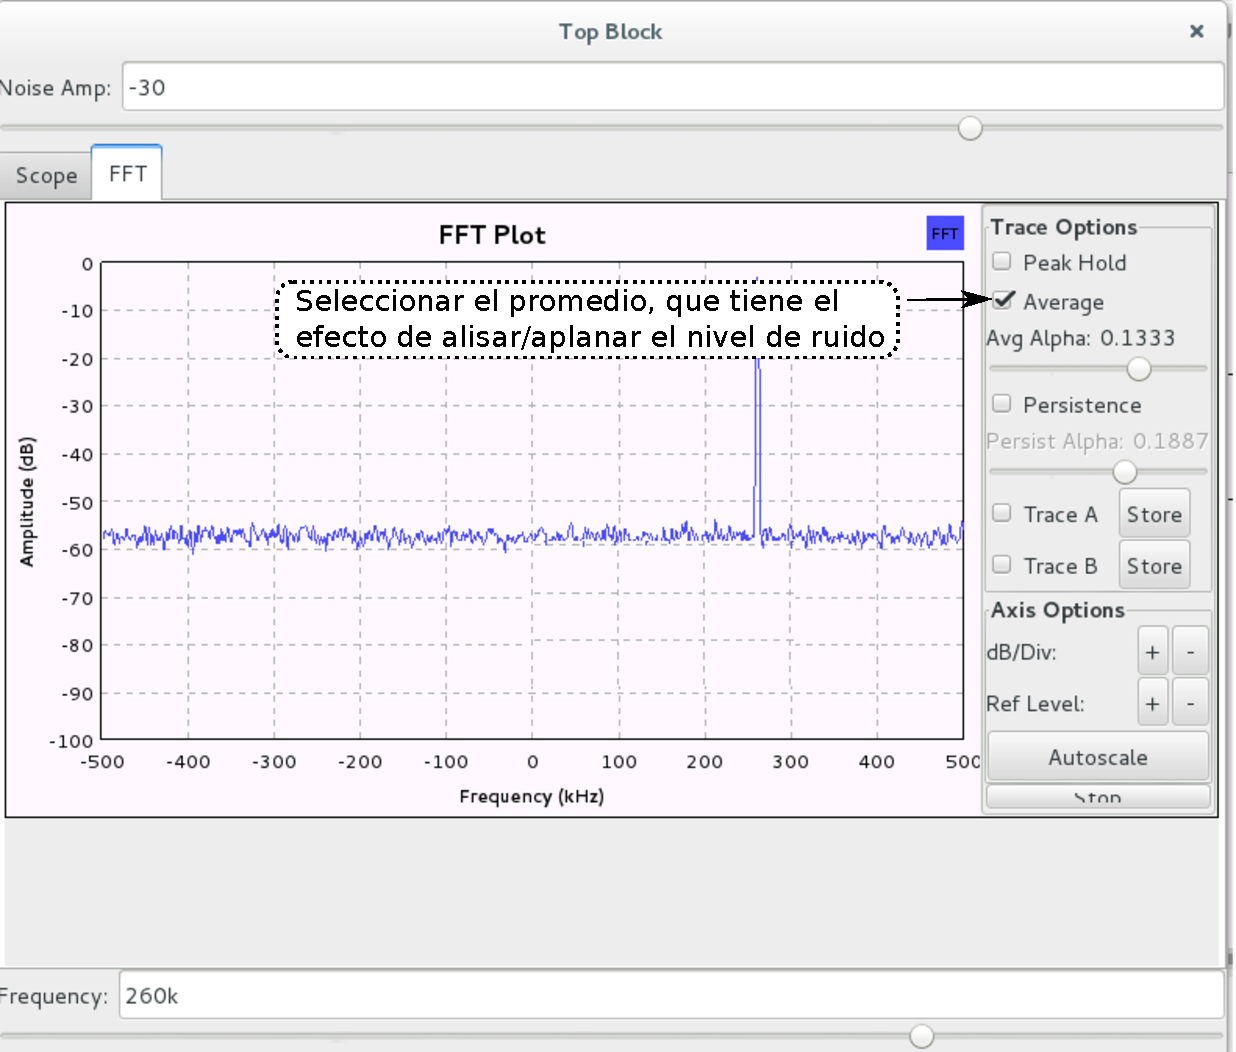
\includegraphics[width=0.75\textwidth]{parte1/lab2/pdf/lab2_11.pdf}
\end{figure}
\end{frame}
%--------------------------------

\begin{frame}{Osciloscopio y FFT}
\begin{figure}[H]
\vspace{-3mm}
\centering
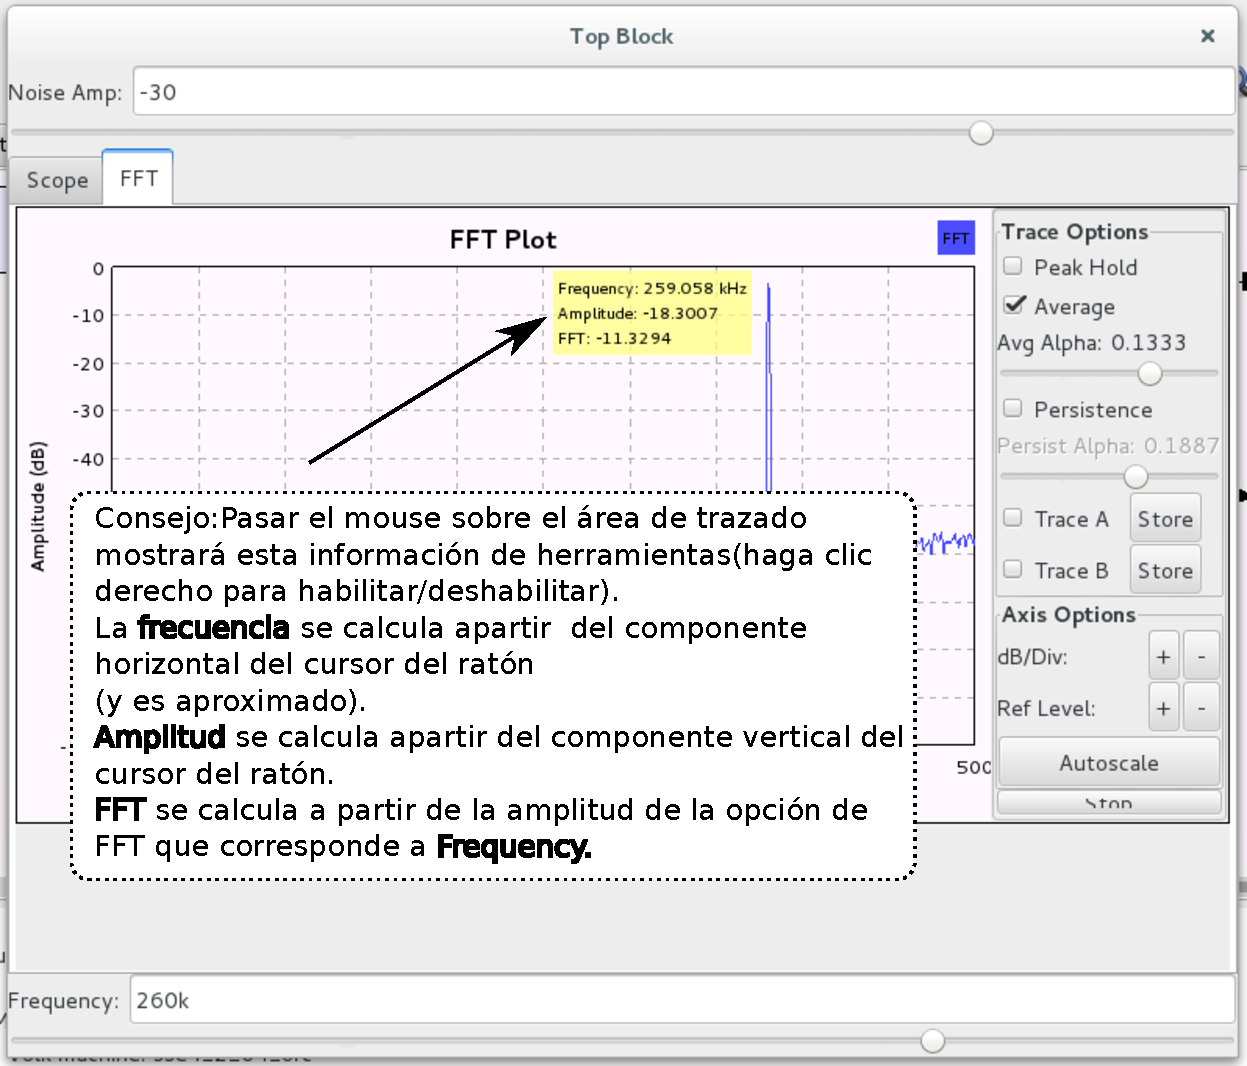
\includegraphics[width=0.75\textwidth]{parte1/lab2/pdf/lab2_12.pdf}
\end{figure}
\end{frame}
%--------------------------------

\begin{frame}{Osciloscopio y FFT}
\begin{figure}[H]
\centering
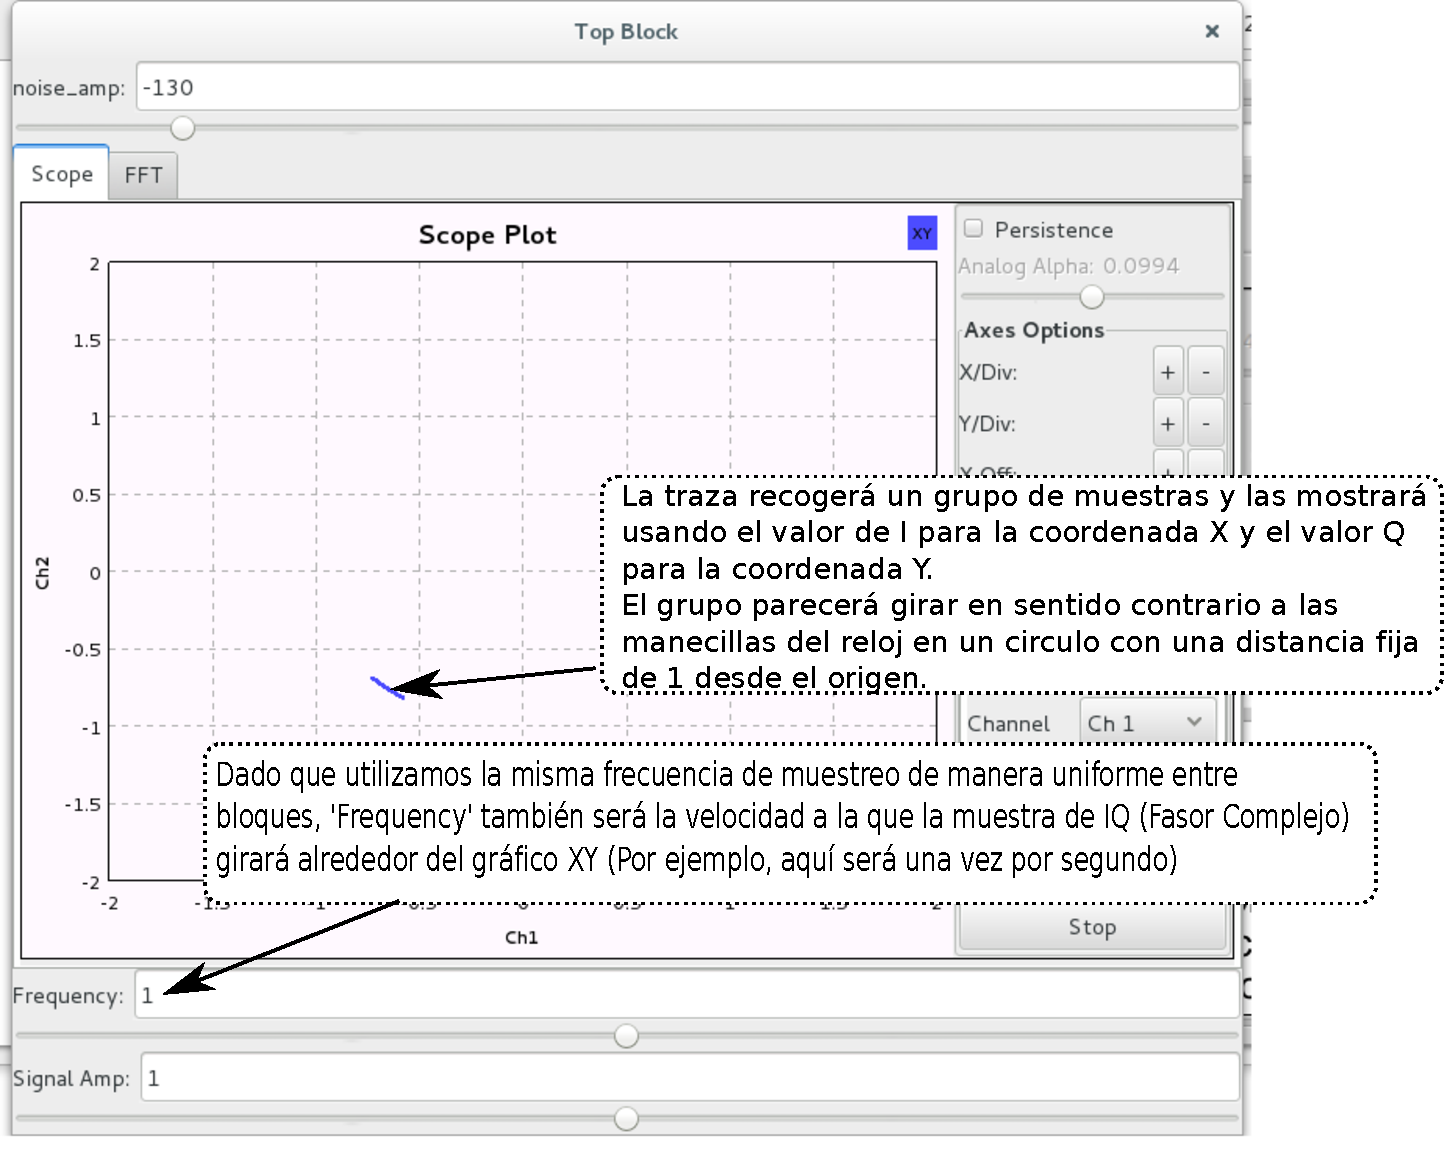
\includegraphics[width=0.75\textwidth]{parte1/lab2/pdf/lab2_13.pdf}
\end{figure}
\end{frame}
%--------------------------------

\begin{frame}{Osciloscopio y FFT}
\begin{figure}[H]
\vspace{-3mm}
\centering
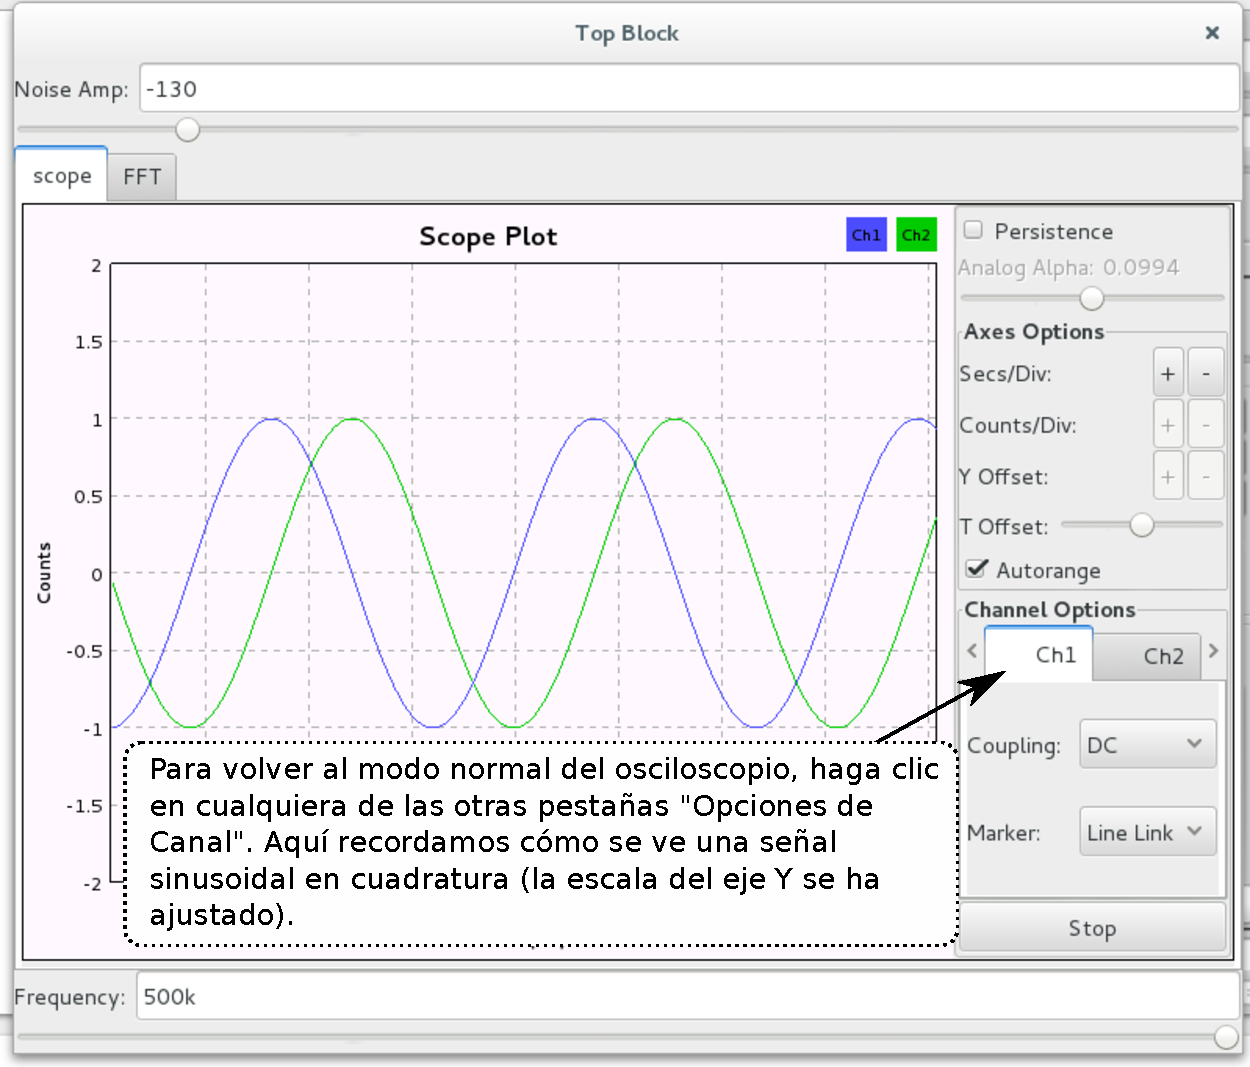
\includegraphics[width=0.75\textwidth]{parte1/lab2/pdf/lab2_14.pdf}
\end{figure}
\end{frame}
%--------------------------------

\begin{frame}{Osciloscopio y FFT}
\begin{figure}[H]
\vspace{-3mm}
\centering
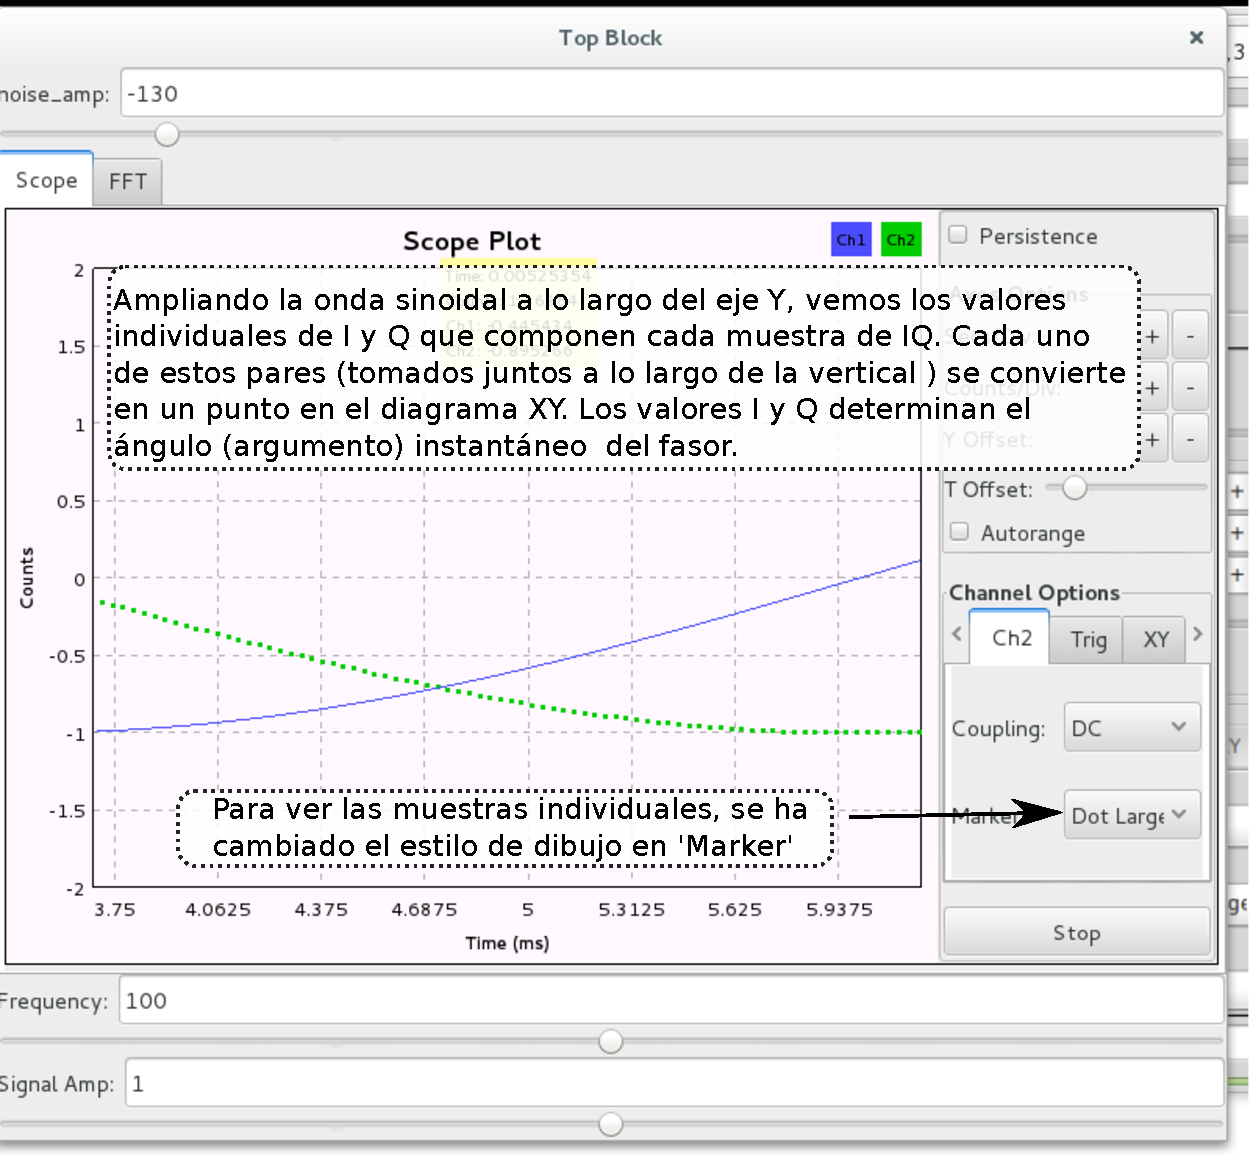
\includegraphics[width=0.7\textwidth]{parte1/lab2/pdf/lab2_15.pdf}
\end{figure}
\end{frame}
%--------------------------------

\begin{frame}{Osciloscopio y FFT}
\begin{figure}[H]
\centering
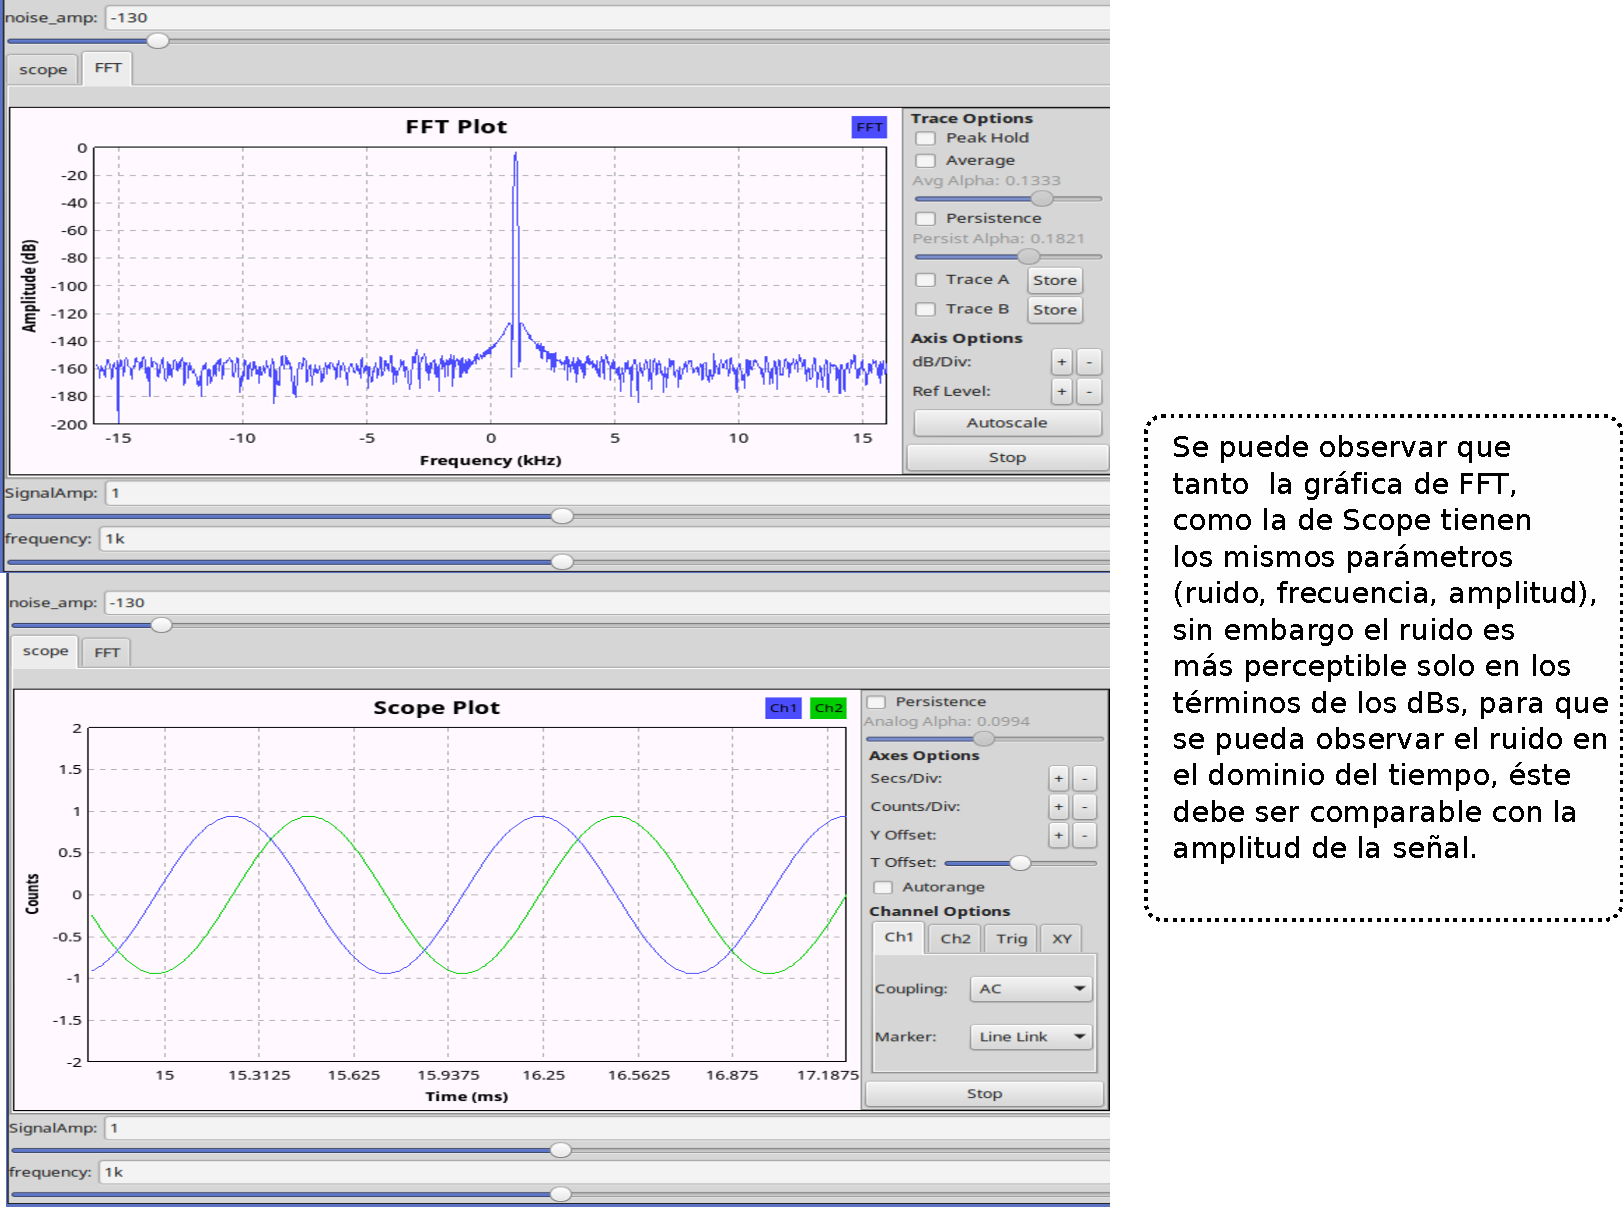
\includegraphics[width=\textwidth, height=0.58\textwidth]{parte1/lab2/pdf/lab2_16.pdf}
\end{figure}
\end{frame}
%--------------------------------

%///////////////////////////////////////////////////////////////

\subsection{Lab3: Audio}
%*********************
\begin{frame}{}

\pgfdeclareimage[width=\paperwidth,height=\paperheight]{bg}{imagenes/fondo_lab}
\setbeamertemplate{background}{\pgfuseimage{bg}}

\bfseries{\textrm{\LARGE Lab3\\ \Large Audio}}
\raggedright
\end{frame}
%*********************

\begin{frame}{Audio \index{Audio}}

\pgfdeclareimage[width=\paperwidth,height=\paperheight]{bg}{imagenes/fondo3}
\setbeamertemplate{background}{\pgfuseimage{bg}}


En esta práctica se generará un tono desde la tarjeta de sonido de la
computadora, originado desde el software y emitido a través de los parlantes
del computador, dicha señal será visualizada desde un osciloscopio, un FFT, y
diagrama de cascada (espectrograma), realizando pruebas de ``loopback'' usando el
micrófono de la computadora.

\end{frame}
%----------------

\begin{frame}{Diagrama:  ``emisión de audio desde la computadora''\index{Audio}}

\begin{figure}

\begin{center}
\vspace{-0.3cm}
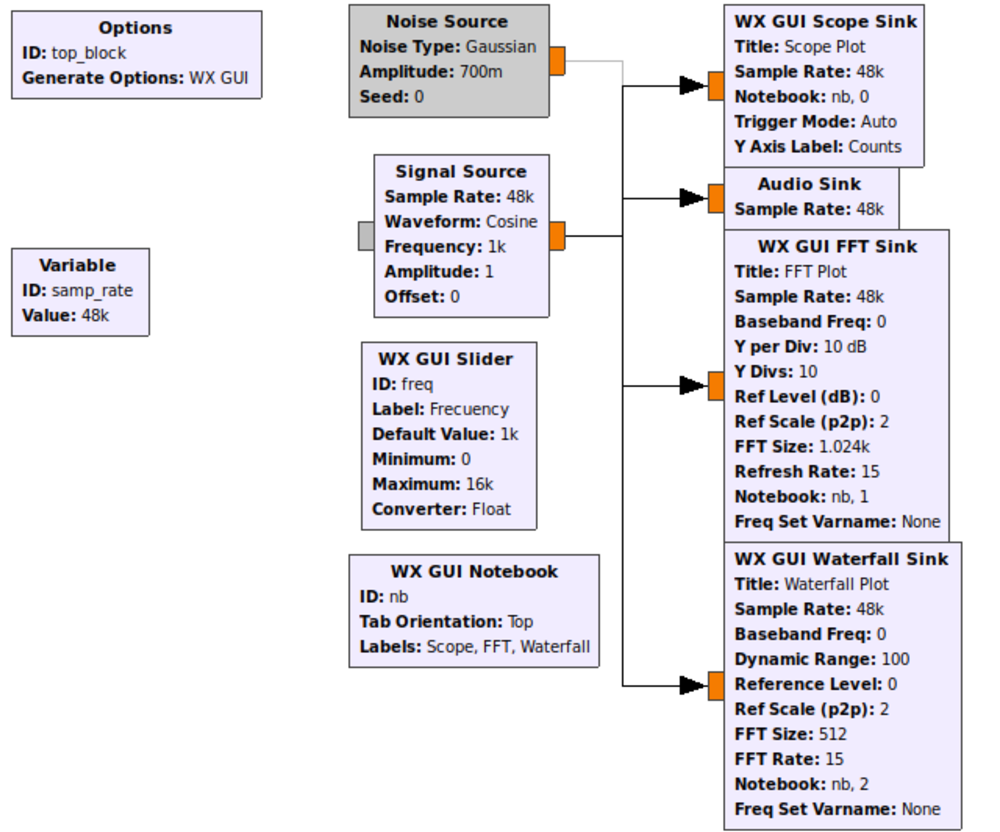
\includegraphics[width=.7\textwidth]{parte1/lab3/pdf/lab3_1.pdf}
\end{center}
\end{figure}

\end{frame}
%----------------

\begin{frame}{Diagrama:  ``emisión de audio desde la computadora''\index{Audio}}

\begin{figure}

\begin{center}
\vspace{-2mm}
    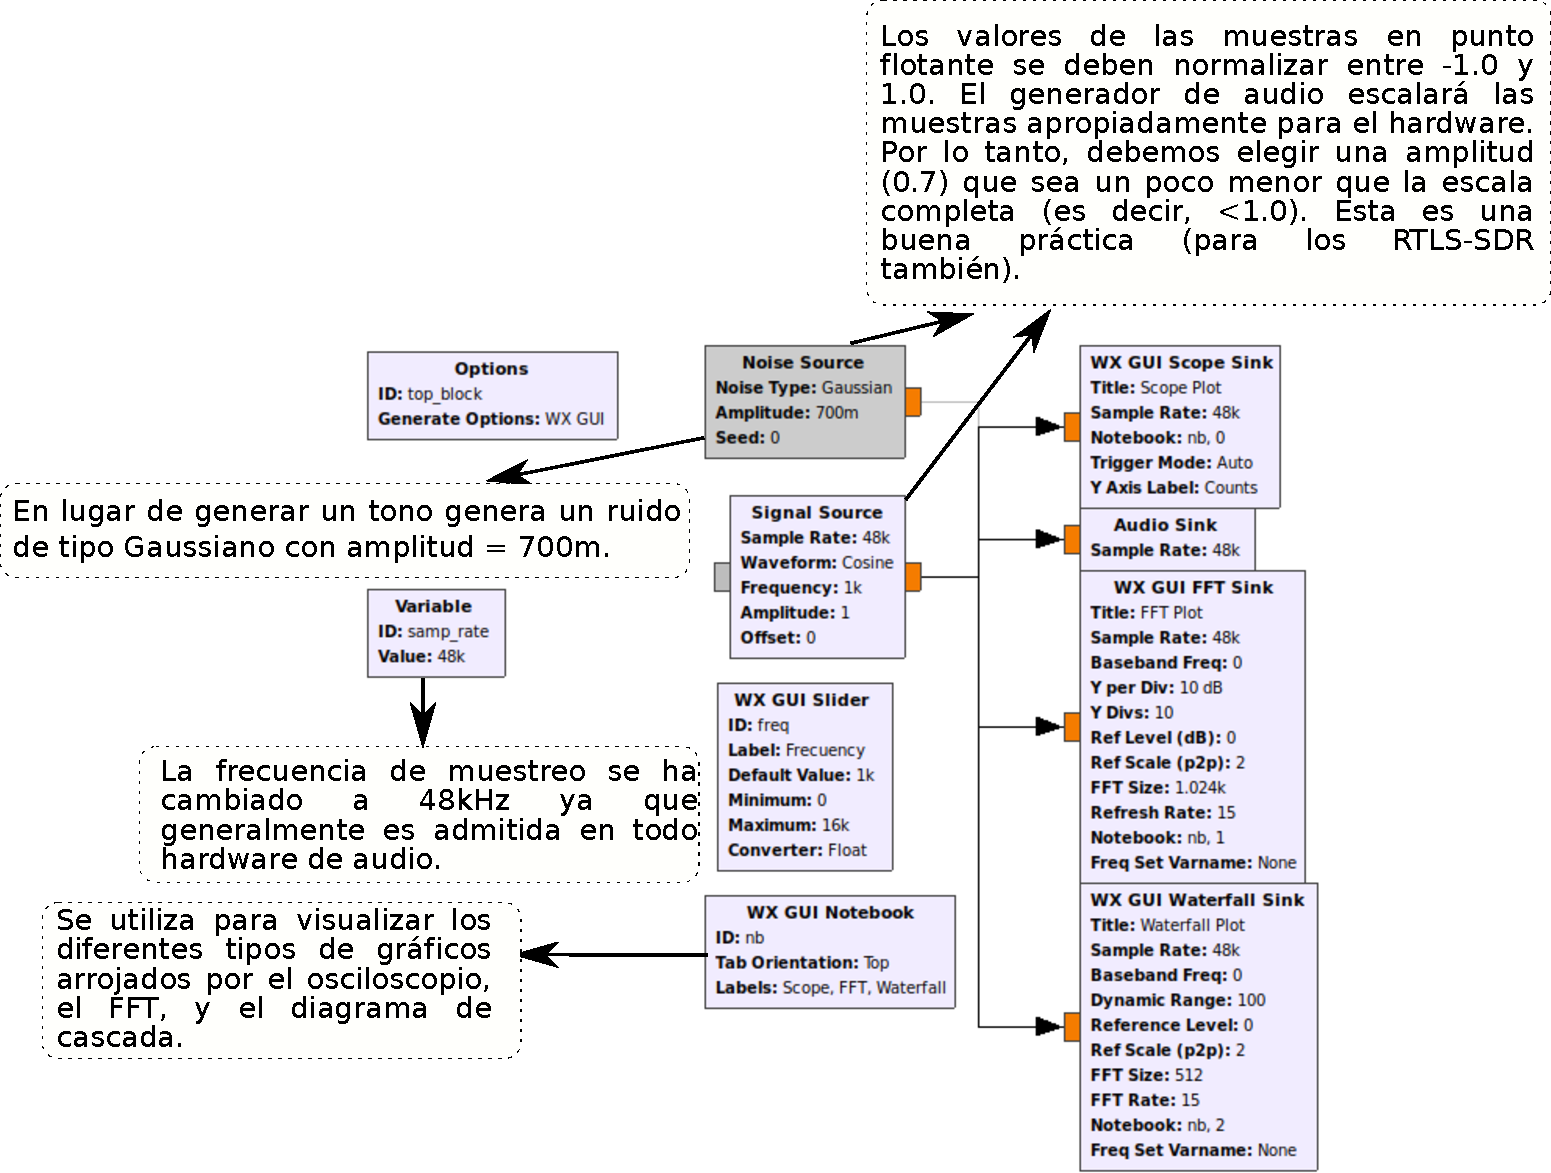
\includegraphics[width=.85\textwidth]{parte1/lab3/pdf/lab3_2.pdf}
\end{center}
\end{figure}

\end{frame}
%----------------

\begin{frame}{Diagrama:  ``emisión de audio desde la computadora''\index{Audio}}

\begin{figure}

\begin{center}
\vspace{-1mm}
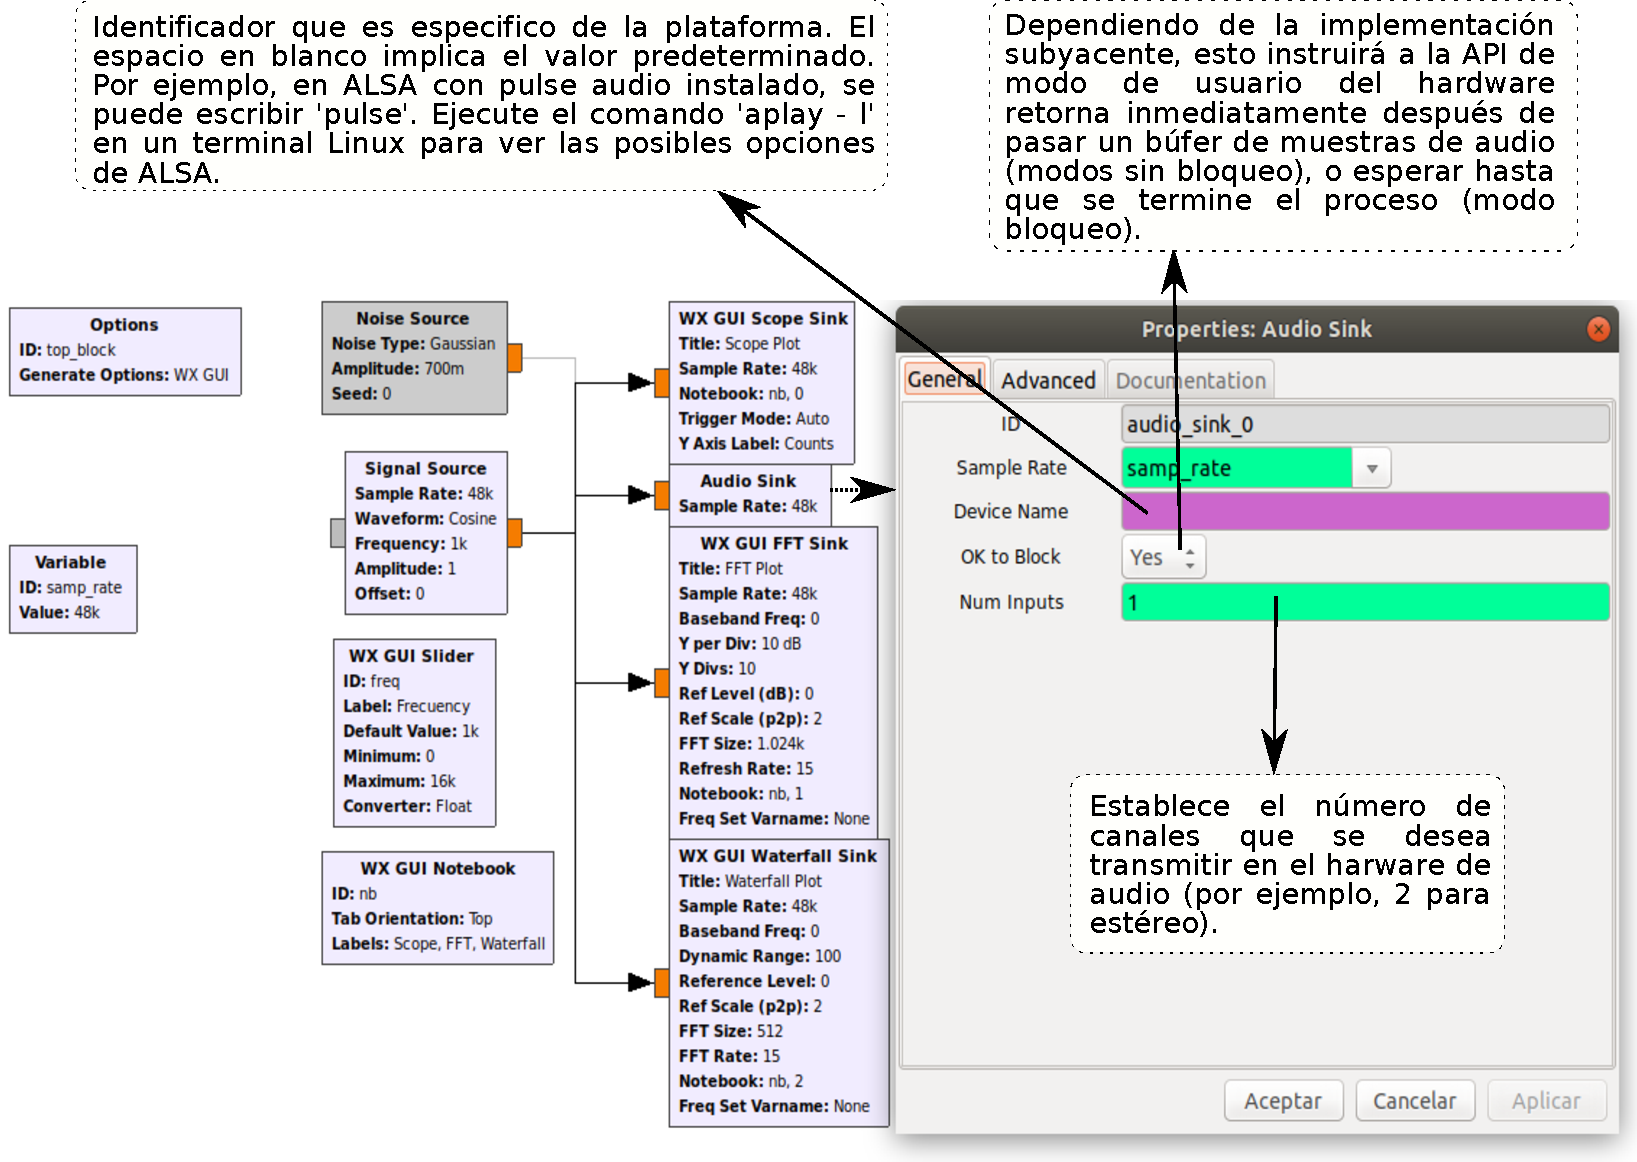
\includegraphics[width=.92\textwidth]{parte1/lab3/pdf/lab3_3.pdf}
\end{center}
\end{figure}

\end{frame}
%----------------

\begin{frame}{Diagrama:  ``emisión de audio desde la computadora''\index{Audio}}

\begin{figure}

\begin{center}
\vspace{-8mm}
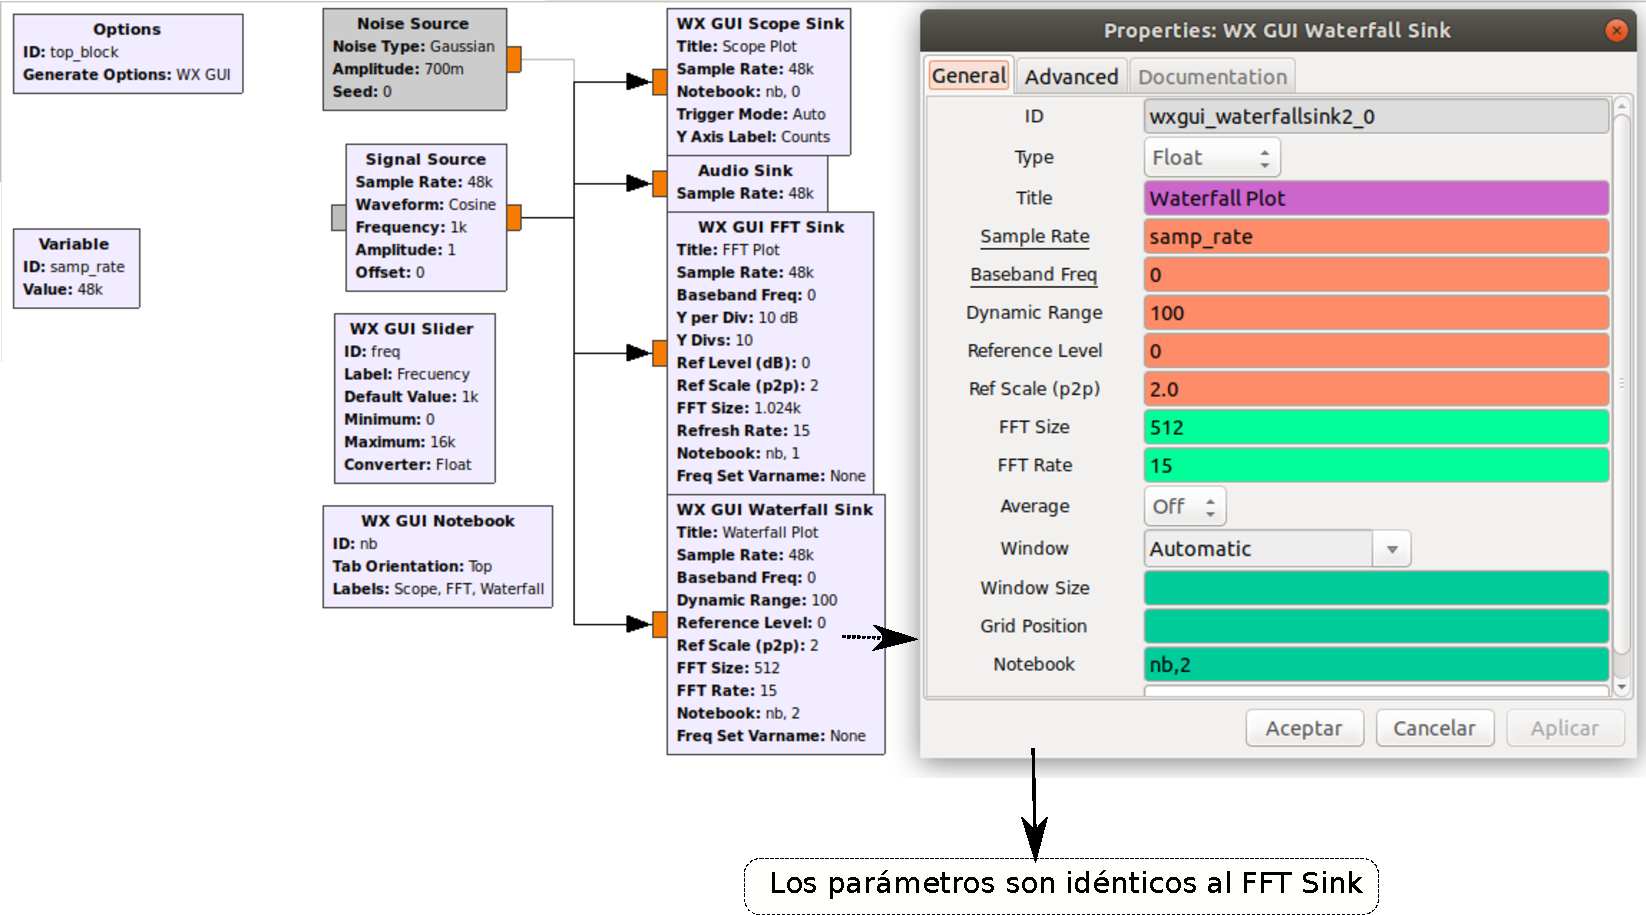
\includegraphics[width=1.05\textwidth]{parte1/lab3/pdf/lab3_4.pdf}
\end{center}
\end{figure}

\end{frame}
%----------------

\begin{frame}{Audio\index{Audio}}

Es importante saber que:\\
\begin{itemize}
    \item
    {Cuando Audio Sink es el único dispositivo hardware en el diagrama de bloques capaz de generar audio, el modo de bloqueo (‘OK to Block’) aplicará un regulador a la producción de muestras del sample\_rate, para que opere eficazmente al reproducir el sonido\cite{Seeber2014}.}
    \item
    {Esto puede ser problemático si la fuente del diagrama de flujo es, por ejemplo, un RTL-SDR. La fuente es también un hardware que tiene su propio reloj interno y será regulado a la tasa de producción de las muestras, mientras que el Audio Sink regula el uso con su propio reloj no sincronizado. Esto se llama el problema de “dos relojes".}
\end{itemize}
\end{frame}
%----------------

\begin{frame}{Audio\index{Audio}}
\begin{itemize}
    \item 
    {Para solucionar este problema de dos relojes, se coloca un regulador de audio en modo sin bloqueo (no dar click ‘Botón de Bloqueo’) de tal forma que nunca interrumpa el diagrama de bloque (es decir, no aplicar el regulador controlado). Esto usará muestras de forma normal, pero si hay un exceso (por ejemplo, el RTL-SDR está produciendo muestras un poco más rápido de lo que el Audio Sink puede usar), se perderán las muestras (podría causar fallas de audio).}
    \item 
    {Esto no soluciona el caso en el que las muestras se producen más lentamente que la tasa de uso del Audio Sink (esto producirá una ejecución lenta: el audio sonará agitado y se imprimirá ‘aU’ en la ventana de registro).}
\end{itemize}



\end{frame}
%----------------

\begin{frame}{Audio\index{Audio}}

\begin{figure}

\begin{center}
\vspace{-7mm}
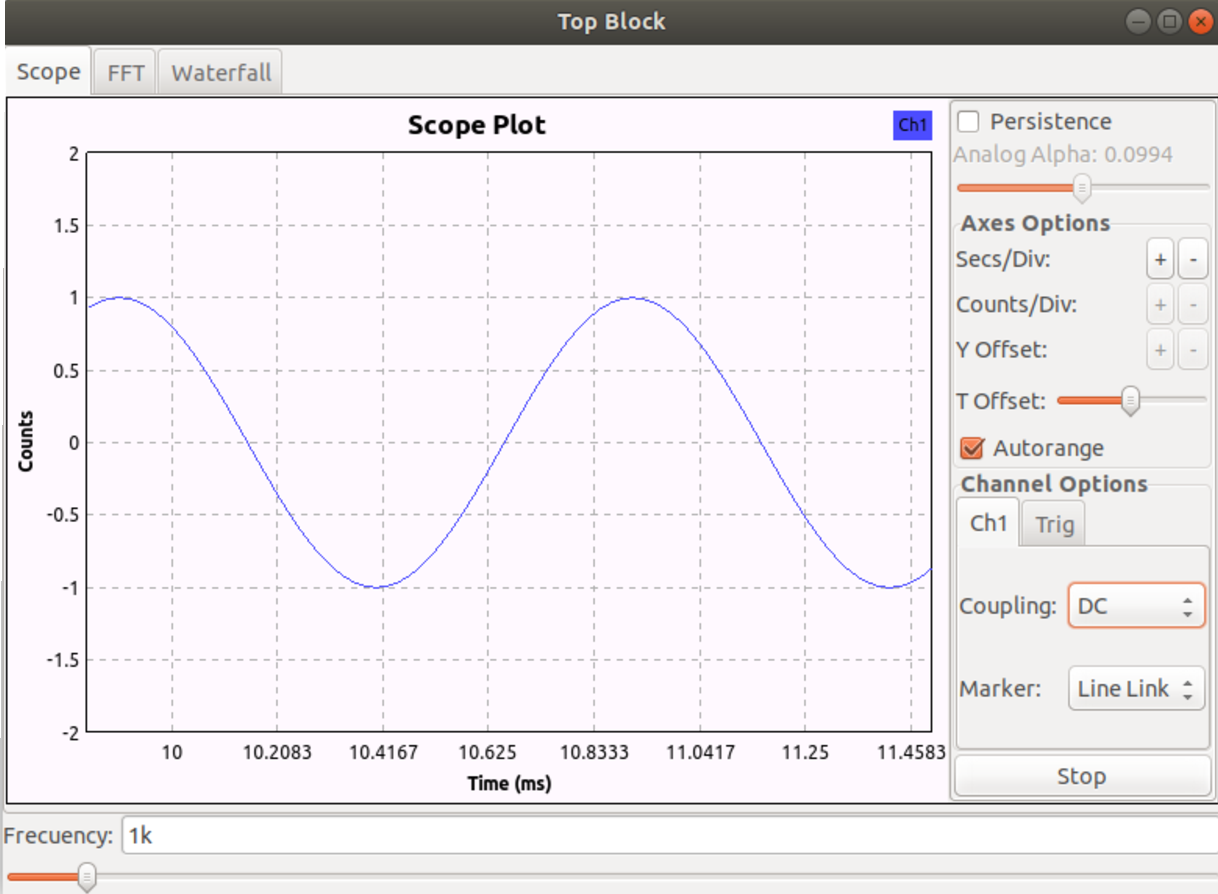
\includegraphics[width=\textwidth, height=0.6\paperheight]{parte1/lab3/pdf/lab3_5.pdf}
\end{center}
\end{figure}
%\tiny
\vspace{-4mm}
La misma onda seno de las prácticas anteriores, pero ahora se puede escuchar emitida por los parlantes del computador.
\end{frame}
%----------------

\begin{frame}{Audio\index{Audio}}

\begin{figure}

\begin{center}
\vspace{-6mm}
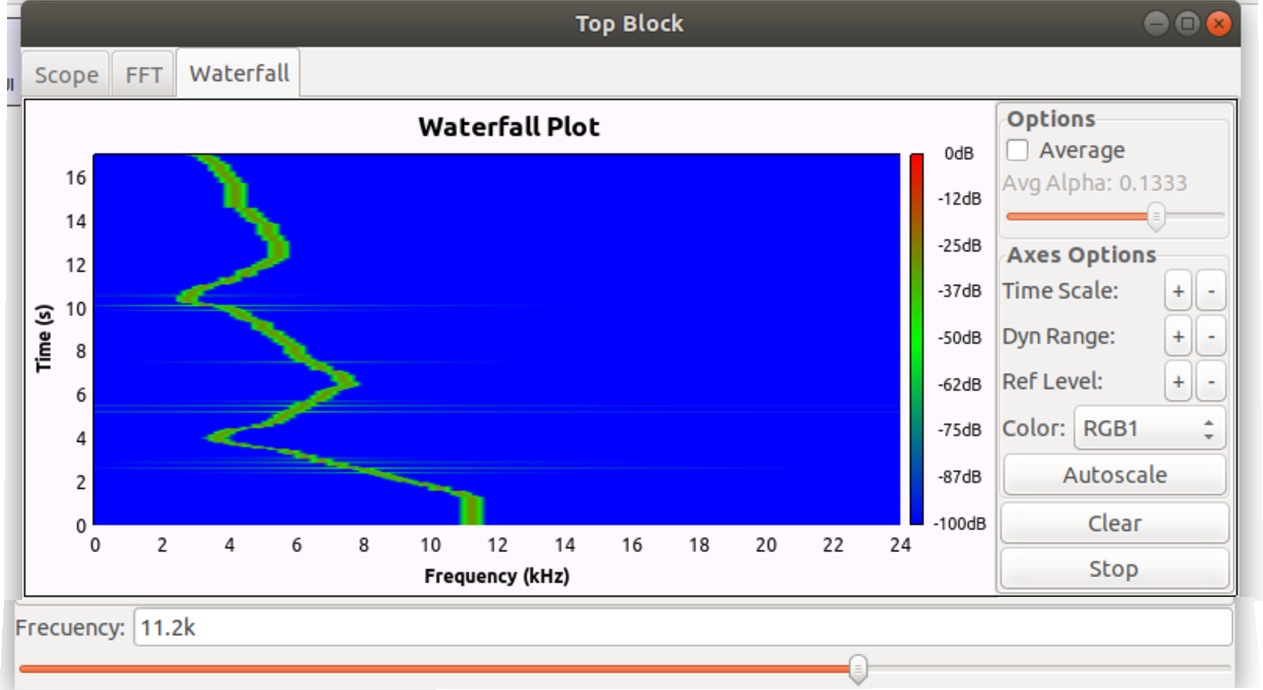
\includegraphics[width=0.8\textwidth]{parte1/lab3/pdf/lab3_6.pdf}
\end{center}
\end{figure}
\vspace{-3mm}

Visualiza el FFT que se desplaza en el tiempo mediante el diagrama de cascada (espectrograma) de la señal emitida. Se añade un bloque de prueba por medio de un generador de señales y un variador deslizante con lo cual se escucha el tono variado en el Audio Sink y poder ver la variación de la frecuencia en el diagrama de cascada.
\end{frame}
%----------------

\begin{frame}{Diagrama: recepción de audio\index{Audio}}

\begin{figure}

\begin{center}
%\vspace{-5mm}
\includegraphics[width=.73\textwidth]{parte1/lab3/pdf/lab3_7.pdf}
\end{center}
\end{figure}

\end{frame}
%----------------

\begin{frame}{Audio\index{Audio}}

\begin{figure}
\begin{center}
\vspace{-8mm}
\includegraphics[width=\textwidth]{parte1/lab3/pdf/lab3_8.pdf}
\end{center}
\end{figure}

Muestra las diferentes señales presentes en el entorno captadas por la tarjeta de audio de la computadora a través del micrófono.

\end{frame}
%----------------

\begin{frame}{Diagrama: prueba con aproximación de “loopback”\index{Audio}}

\begin{figure}
\begin{center}
\vspace{-6mm}
\includegraphics[width=\textwidth, height=0.6\paperheight]{parte1/lab3/pdf/lab3_9.pdf}
\end{center}
\end{figure}
\vspace{-5mm}
Ejecutando el programa generador de onda sinusoidal al mismo tiempo, y cambiando la frecuencia. Se trata de una prueba aproximada de “loopback" en la que el micrófono de la computadora escucha sus altavoces.

\end{frame}
%----------------

\begin{frame}{Audio\index{Audio}}

\begin{figure}
\begin{center}
\vspace{-8mm}
\includegraphics[width=\textwidth, height=0.6\paperheight]{parte1/lab3/pdf/lab3_10.pdf}
\end{center}
\end{figure}
\vspace{-5mm}
Con la realimentación de las entradas micrófono-altavoces y generación de señal a través de la tarjeta de audio de la computadora.

\end{frame}
%---------------


%///////////////////////////////////////////////////////////////

\subsection{Lab4: Modulación ASK en GRC}

%*********************
\begin{frame}{}

\pgfdeclareimage[width=\paperwidth,height=\paperheight]{bg}{imagenes/fondo_lab}
\setbeamertemplate{background}{\pgfuseimage{bg}}

\bfseries{\textrm{\LARGE Lab4\\ \Large Modulación ASK en GRC}}
\raggedright
\end{frame}
%*********************

%--------------------------

\begin{frame}{Modulación ASK en GRC}


\pgfdeclareimage[width=\paperwidth,height=\paperheight]{bg}{imagenes/fondo3}
\setbeamertemplate{background}{\pgfuseimage{bg}}

  \begin{itemize}
  \item {
En esta práctica se hace uso de la  Modulación por desplazamiento de amplitud (ASK) este es un esquema de modulación digital en el que la amplitud de la onda portadora se cambia con respecto a la señal de información, manteniendo la fase y la frecuencia de constantes. Para el presente laboratorio, se utilizó BASK, el cual tiene el mismo comportamiento, pero utilizando bits. Donde su comportamiento es descrito por la siguiente ecuación:

\begin{equation*}
S(t) = Am(t)cos(wt)
\end{equation*}

  }
  \item {
El diagrama de bloques en GRC consiste en la multiplicación de una señal de información con una portadora, que corresponde a una señal coseno de diez veces la frecuencia de la información. La frecuencia de muestreo debe ser mayor que el doble de la frecuencia máxima de la señal de datos.
  }
  \end{itemize}
\end{frame}
%---------------------------

\begin{frame}{Modulación ASK en GRC}

\begin{figure}[H]
\centering
\includegraphics[width=\textwidth]{parte1/lab4/pdf/lab4_1.pdf}
\end{figure}
Diagrama de bloques en GNU radio, para generar una modulación ASK entre dos señales.
\end{frame}
%--------------------

\begin{frame}{Modulación ASK en GRC}
\vspace{-1cm}
\begin{figure}[H]
\centering
\includegraphics[width=1.1\textwidth]{parte1/lab4/pdf/lab4_2.pdf}
\end{figure}
\end{frame}
%_---------------------

\begin{frame}{Modulación ASK en GRC}
\vspace{-1.5cm}
\begin{figure}[H]
\centering
\includegraphics[width=1.1\textwidth]{parte1/lab4/pdf/lab4_3.pdf}
\end{figure}
\end{frame}
%_---------------------

\begin{frame}{Modulación ASK en GRC}

  \begin{itemize}
  \item {
La Modulación por desplazamiento de frecuencia (FSK) es una técnica de modulación digital, utilizada para la transmisión de datos. Para BFSK que corresponde al mismo proceso, pero con datos binarios, se utilizan dos frecuencias diferentes para transmitir dos señales, es decir 0 y 1. como se puede ver a continuación:

\begin{equation*}
S_{1}(t) = Acos(w_{1}t)
\end{equation*}

\begin{equation*}
S_{2}(t) = Acos(w_{2}t)
\end{equation*}

  }
  \item {
El diagrama de boques en GRC se utilizaron dos señales coseno como portadora de amplitud 1, y frecuencias de 1Khz y 10Khz. La señal 1 es representada por una onda cuadrada, y la señal 0 es obtenida restándole 1 a la señal cuadrada. Posteriormente se multiplican las señales 0 y 1 con las portadoras y luego se suman obteniendo la modulación FSK.
  }
  \end{itemize}
\end{frame}
%---------------------------


\begin{frame}{Modulación ASK en GRC}
\vspace{-8mm}
\begin{figure}[H]
\centering
\includegraphics[width=\textwidth]{parte1/lab4/pdf/lab4_4.pdf}
\end{figure}
\end{frame}
%_---------------------

\begin{frame}{Modulación ASK en GRC}
\begin{figure}[H]
\centering
\includegraphics[width=\textwidth]{parte1/lab4/pdf/lab4_5.pdf}
\end{figure}
\end{frame}
%_---------------------

\begin{frame}{Modulación ASK en GRC}
\begin{figure}[H]
\centering
\includegraphics[width=\textwidth]{parte1/lab4/pdf/lab4_6.pdf}
\end{figure}
\end{frame}
%_---------------------

\begin{frame}{Modulacion ASK en GRC}

  \begin{itemize}
  \item {
La Modulación por desplazamiento de fase (PSK) es un esquema de modulación digital donde se varía la fase de la señal, manteniendo la frecuencia y la amplitud constante. Para la modulación PSK se usan dos señales con fases diferentes y frecuencias iguales, estas se multiplican con la señal 0 o 1 de los datos como se muestra a continuación:

\begin{equation*}
S_{1}(t) = Acos(wt)
\end{equation*}

\begin{equation*}
S_{2}(t) = Acos(wt)
\end{equation*}

  }
  \item {
El diagrama de boques en GRC se utiliza una señal coseno de 50000 Hz y la amplitud pico de 1, y otra onda sinusoidal de igual frecuencias y amplitud. Similar a BFSK se representa la señal 1 con la onda cuadrada de frecuencia 5000 Hz y el 0 por la resta de la constante.
  }
  \end{itemize}
\end{frame}
%---------------------------

\begin{frame}{Modulación ASK en GRC}
\begin{figure}[H]
\centering
\includegraphics[width=\textwidth]{parte1/lab4/pdf/lab4_7.pdf}
\end{figure}
\end{frame}
%_---------------------

\begin{frame}{Modulación ASK en GRC}
\begin{figure}[H]
\centering
\includegraphics[width=\textwidth]{parte1/lab4/pdf/lab4_8.pdf}
\end{figure}
\end{frame}
%_---------------------
\begin{frame}{Modulación ASK en GRC}
\begin{figure}[H]
\centering
\includegraphics[width=\textwidth]{parte1/lab4/pdf/lab4_9.pdf}
\end{figure}
\end{frame}
%_---------------------

%///////////////////////////////////////////////////////////////

\subsection{Lab5: Modulación BPSK en GRC}

%*********************
\begin{frame}{}

\pgfdeclareimage[width=\paperwidth,height=\paperheight]{bg}{imagenes/fondo_lab}
\setbeamertemplate{background}{\pgfuseimage{bg}}

\bfseries{\textrm{\LARGE Lab5\\ \Large Modulación BPSK en GRC}}
\raggedright
\end{frame}
%*********************

%--------------------------

\begin{frame}{Modulación BPSK en GRC}


\pgfdeclareimage[width=\paperwidth,height=\paperheight]{bg}{imagenes/fondo3}
\setbeamertemplate{background}{\pgfuseimage{bg}}


En esta práctica se hace uso de la modulación de desplazamiento de fase de 2 símbolos. Es el más sencillo de todos, puesto que solo emplea 2 símbolos, con 1 bit de información cada uno. Es también la que presenta mayor inmunidad al ruido, puesto que la diferencia entre símbolos es máxima (180º). Dichos símbolos suelen tener un valor de salto de fase de 0º para el 1 y 180º para el 0, como se muestra en un diagrama de constelación.
  

\end{frame}
%---------------------------

\begin{frame}{Modulación BPSK en GRC}

\begin{figure}
  \centering
   \includegraphics[width=\textwidth]{parte1/lab5/pdf/lab5_1.pdf}
  \end{figure}
  
\end{frame}
%------------------------

\begin{frame}{Modulación BPSK en función del tiempo}
\begin{figure}[H]
\centering
\includegraphics[width=.7\textwidth]{parte1/lab5/pdf/lab5_2.pdf}
\end{figure}
Convierte el flujo de datos digital en señal analógica de banda base (muestreada) utilizando el filtro FIR de interpolación.
\end{frame}
%------------------------

\begin{frame}{Modulación BPSK en GRC}
\begin{figure}[H]
\centering
\includegraphics[width=.7\textwidth]{parte1/lab5/pdf/lab5_3.pdf}
\end{figure}
\end{frame}
%------------------------

\begin{frame}{Modulación BPSK en función del tiempo}
\begin{figure}[H]
\centering
\includegraphics[width=.8\textwidth]{parte1/lab5/pdf/lab5_4.pdf}
\end{figure}
\end{frame}
%------------------------

\begin{frame}{Modulación BPSK en GRC}
\begin{figure}[H]
\centering
\includegraphics[width=\textwidth]{parte1/lab5/pdf/lab5_5.pdf}
\end{figure}
\end{frame}
%------------------------

\begin{frame}{Modulación BPSK en GRC}
\vspace{-8mm}
\begin{figure}[H]
\centering
\includegraphics[width=.9\textwidth]{parte1/lab5/pdf/lab5_6.pdf}
\end{figure}
\tiny
Se deshabilita el bloque del osciloscopio WX GUI y se habilita el osciloscopio de constelaciones QT GUI , también se debe cambiar en el bloque Options: Generate options: WX GUI por QT GUI para que el bloque de constelaciones funcione.
\end{frame}
%------------------------

\begin{frame}{Constelación BPSK}
\begin{figure}[H]
\centering
\includegraphics[width=\textwidth]{parte1/lab5/pdf/lab5_7.pdf}
\end{figure}
\end{frame}
%------------------------
%///////////////////////////////////////////////////////////////

%\section{BIBLIOGRAFÍA}
\begin{frame}

\pgfdeclareimage[width=\paperwidth,height=\paperheight]{bg}{imagenes/fondo_seccion}
\setbeamertemplate{background}{\pgfuseimage{bg}}

\definecolor{greenU}{RGB}{212,202,72}
\setbeamercolor{block body}{fg=Black,bg=greenU}
\begin{block}{}
\centering
\vspace{8mm}
\Large{BIBLIOGRAFÍA}
\vspace{8mm}
\end{block}
\end{frame}
%-----------------------

\begin{frame}[allowframebreaks]
\frametitle{Referencias}

\pgfdeclareimage[width=\paperwidth,height=\paperheight]{bg}{imagenes/fondo3}
\setbeamertemplate{background}{\pgfuseimage{bg}}

\bibliographystyle{unsrt}
\begin{thebibliography}{9}







%-----
\bibitem{Seeber2014} Seeber, Balint.
\newblock "GNU Radio Tutorials Labs 1 – 5". [Online] \url{https://files.ettus.com/tutorials/labs/Lab\_1-5.pdf}. 

%-----
\bibitem{Conferencia2015} Vachhani, Khyati. Gokhruwala, Kenil; Kumar, Jay  
\newblock "Design Analysis of Digital Modulation Schemes with GNU Radio". [Descargado de:] \url{https://www.researchgate.net/publication/281106848_Design_Analysis_of_Digital_Modulation_Schemes_with_GNU_Radio}. 

%-----
\bibitem{Wikipedia8} Wikipedia.
\newblock "Frecuencia modulada". [Online] \url{https://es.wikipedia.org/wiki/Frecuencia_modulada}. 

%-----
\bibitem{linuxjournal1995} Vaught, Andy.
\newblock "Introduction to Named Pipes". [Online] \url{https://www.linuxjournal.com/article/2156}. 

%-----
\bibitem{wikiopendigital} Wiki Opendigitalradio.
\newblock "Simple FM transmitter using gnuradio". [Online] \url{http://wiki.opendigitalradio.org/Simple_FM_transmitter_using_gnuradio}. 

%-----

\bibitem{FichaTecnica} Electronisys.
\newblock "Ficha técnica de radio portátil UHF Motorola EP150". [Descargado de:] \url{http://www.electronisys.cl/index.php?route=product/product&product\_id=50}. 

%-----
\bibitem{Wikipedia2018} Wikipedia.
\newblock "Continuous Tone-Coded Squelch System". [Online] \url{https://en.wikipedia.org/wiki/Continuous\_Tone-Coded\_Squelch\_System}. 

%-----
\bibitem{Airspy2018} Airspy.
\newblock "Airspy Redefining the Radio Experience". [Online] \url{https://airspy.com/download/}

%-----
\bibitem{Motorola2010} Motorola Solutions.
\newblock "Two-Way Radios". [Online] \url{https://www.motorolasolutions.com/content/dam/msi/docs/enxl/products/two-way-radios-business/portable-radios/on-site-smallbusiness/}. 

%-----
\bibitem{Lecture9} Documento PDF
\newblock "Lecture 9 Analog and Digital I/Q Modulation". [Online] \url{http://web.mit.edu/6.02/www/f2006/handouts/Lec9.pdf}.





\end{thebibliography}


\end{frame}


%\end{document}


%/////////////////////////

\section{CONFIGURACIÓN E INSTALACIÓN DE HARDWARE}
\begin{frame}

\pgfdeclareimage[width=\paperwidth,height=\paperheight]{bg}{imagenes/fondo_seccion}
\setbeamertemplate{background}{\pgfuseimage{bg}}

\definecolor{greenU}{RGB}{212,202,72}
\setbeamercolor{block body}{fg=Black,bg=greenU}
\begin{block}{}
\centering
\vspace{8mm}
\Large{CONFIGURACIÓN E INSTALACIÓN DE HARDWARE}
\vspace{8mm}
\end{block}
\end{frame}
%-----------------------

{
\begin{frame}
\frametitle{Parte II - Tabla de contenidos}
\begin{spacing}{1.5}
\tableofcontents[currentsection,sectionstyle=hide/hide,subsectionstyle=show/show/hide, subsubsectionstyle=hide]
\end{spacing}
\end{frame}
}


\subsection{Lab6: RTL}
%*********************
\begin{frame}{}

\pgfdeclareimage[width=\paperwidth,height=\paperheight]{bg}{imagenes/fondo_lab}
\setbeamertemplate{background}{\pgfuseimage{bg}}

\bfseries{\textrm{\LARGE Lab6\\ \Large RTL}}
\raggedright
\end{frame}
%*********************

\begin{frame}{RTL\_SDR}

\pgfdeclareimage[width=\paperwidth,height=\paperheight]{bg}{imagenes/fondo3}
\setbeamertemplate{background}{\pgfuseimage{bg}}


El RTL\_SDR es un dispositivo el cual permite combinar tanto la parte de software como hardware para implementar un sistema con el cual sea posible desarrollar procesos de radiocomunicaciones tanto de recepción como de transmisión de señales.\\ \vspace{2mm}
El RTL se creó principalmente para solucionar los problemas de compilación para equipos con procesamiento de Pentium 4, esta tarjeta está diseñada para poder demodular señales en FM, AM y SSB con diferentes anchos de banda; también tiene la capacidad de analizar más de cien frecuencias en un segundo.\\\vspace{2mm}
En general el RTL es una gran ayuda a nivel educativo ya que ayuda a hacer una estación receptora si no se tiene una.


\end{frame}
%----------------
\begin{frame}{Instalación de paquetes}

En la siguiente guía práctica se dará un ejemplo por medio de uso de terminal y órdenes, para la captura de señales de radio FM, escáner de la policía, airband scanner y decodificador de localización.

\end{frame}
%------------------------

\begin{frame}
\frametitle{Instalación de Paquetes}

Para instalar los paquetes desde consola se debe ingresar las siguientes órdenes.

\textbf{Paquetes de SOX}
\begin{itemize}
 
    \item { Mediante esta órden, es posible la descarga de las librerías o paquetes necesarios para el correcto y completo funcionamiento de SOX.
    \begin{block}{}
    \texttt
    {\ \ \ root@user\~\$ sudo apt-get install libsox-fmt-alsa}
    \end{block}}
    
    \item{Este paquete contiene la mayoría de las bibliotecas de formatos de audio compatibles con SOX
    \begin{block}{}
    \texttt
    {\ \ \ root@user\~\$ sudo apt-get install libsox-fmt-base}
    \end{block}}
\end{itemize}

\end{frame}
%--------------------------

\begin{frame}
\frametitle{Instalación de Paquetes}

\begin{itemize}
    \item {Este paquete contiene la biblioteca sox que permite convertir varios formatos de archivos de audio de computadora en otros formatos.
    \begin{block}{}
    \texttt
    {\ \ \ root@user\~\$ sudo apt-get install libsox2}
    \end{block}}
    
    \item{SOX es una herramienta conocida como “la navaja suiza” en manipulación de audio, ya que contiene las bibliotecas I/O que permiten el procesamiento del audio en diversos formatos.
    \begin{block}{}
    \texttt
    {\ \ \ root@user\~\$ sudo apt-get install sox}
    \end{block}}
\end{itemize}

\end{frame}
%--------------------------

\begin{frame}
\frametitle{Instalación de Paquetes}

\begin{itemize}
    \item {Este paquete contiene una biblioteca compartida.
    \begin{block}{}
    \texttt
    {\ \ \ root@user\~\$ sudo apt-get install libgnuradio-osmosdr0.1.4}
    \end{block}}
    
    \item{Este paquete es el software que proporciona el control del hardware USB e independientemente de la API, pasar datos a aplicaciones de radio definidas por software en el host. Tiene la posibilidad de recibir o transmitir información.
    \begin{block}{}
    \texttt
    {\ \ \ root@user\~\$ sudo apt-get install libosmosdr0}
    \end{block}}
\end{itemize}

\end{frame}
%--------------------------

\begin{frame}
\frametitle{Instalación de Paquetes}
\textbf{Paquetes de RTL\_SDR}
\begin{itemize}
 
    \item { Es un software que soporta dispositivos SDR tales como Airspy, funcube Dongles, rtl-sdr, HackRF, y USRP
    \begin{block}{}
    \texttt
    {\ \ \ root@user\~\$ sudo apt-get install gqrx-sdr}
    \end{block}}
     \item { Este archivo contiene librerías y archivos de desarrollo que complemetan el funcionamiento de conexión de la RTL.
    \begin{block}{}
    \texttt
    {\ \ \ root@user\~\$ sudo apt-get install librtlsdr-dev}
    \end{block}}
\end{itemize}

\end{frame}
%--------------------------

\begin{frame}
\frametitle{Instalación de Paquetes}
\begin{itemize}
 
    \item {Este paquete contiene una biblioteca compartida.
    \begin{block}{}
    \texttt
    {\ \ \ root@user\~\$ sudo apt-get install librtlsdr0}
    \end{block}}
    \item {Este paquete permite el recepcionamiento I/Q para dispositivos basados en la RTL2832. 
    \begin{block}{}
    \texttt
    {\ \ \ root@user\~\$ sudo apt-get install rtl-sdr}
    \end{block}}
\end{itemize}

\end{frame}
%--------------------------

\begin{frame}
\frametitle{Procedimiento}

Para iniciar es necesario abrir una nueva terminal, desde allí se realizará el procedimiento para comprobar la conexión del hardware RTL con su computadora. \vspace{2mm}
Se debe ingresar la siguiente orden:

\begin{block}{}
    \texttt
    {\ \ \ root@user\~\$ rtl\_test}
    \end{block}

\texttt{rtl\_test} es una herramienta verificadora de la conexión para receptores DVB-T basados en RTL2832. \\ \vspace{2mm}
Si existe una respuesta satisfactoria evidenciará el siguiente mensaje:

\begin{block}{}
    \texttt
    {Info: This tool will continuously read from the device, and report if samples get lost. If you observe no further output, everything is fine. Reading samples in async mode... cb transfer status: 1, canceling...}
    \end{block}

\end{frame}
%--------------------------

\begin{frame}
\frametitle{Procedimiento}

Si el hadware RTL no está conectado evidenciará el siguiente mensaje:

\begin{block}{}
    \texttt
    {No supported devices found.}
    \end{block}

Al conectar mas de un dispositivo RTL y ejecutar la orden \texttt{rtl\_test}, se visualiza un listado de los dispositivos con sus respectivas referencias, como se muestra a continuación.
    
    \begin{block}{}
    \texttt
    {Found 2 device(s):\\
    0:  Realtek, RTL2838UHIDIR, SN: 00000001\\ 
    1:  Realtek, RTL2838UHIDIR, SN: 00000001\\
    Using device 0: Generic RTL2832U OEM\\ 
    Found Rafael Micro R820T tuner\\ 
    Supported gain values (29): 0.0 0.9 1.4 2.7 3.7 7.7 8.7 12.5 14.4 15.7 16.6 19.7 20.7 22.9 25.4 28.0 29.7 32.8 33.8 36.4 37.2 38.6 40.2 42.1 43.4 43.9 44.5 48.0 49.6\\
    {[R82XX]} PLL not locked!\\
    Sampling at 2048000 S/s. 
}
    \end{block}

\end{frame}
%--------------------------

\begin{frame}
\frametitle{Procedimiento}

Al ser desconectada la RTL mientras se ejecuta el test lo notifica mediante el siguiente mensaje: 

\begin{block}{}
    \texttt{
    Reading samples in async mode... \\
    lost at least 84 bytes \\
    cb transfer status: 5, canceling... \\
    cb transfer status: 5, canceling... \\
    cb transfer status: 5, canceling... \\
    cb transfer status: 5, canceling... \\
    cb transfer status: 5, canceling... \\\vspace{2mm}
    Library error -5, exiting…\\}
\end{block}

\end{frame}
%--------------------------

\begin{frame}
\frametitle{Procedimiento}

\textbf{Receptor de Radio Pública FM}\\
\vspace{2mm}
Para esta práctica se debe realizar desde la terminal, puede utilizar la misma o abrir una nueva. Se ingresa la siguiente órden:

\begin{block}{}
  \texttt{
  \ \ \ root@user\~\$ rtl\_fm -M wbfm -f 103.3M -s 1000k -l 0
    \begin{itemize}
      \item[] {|play -r 32k -t raw -e s -b 16 -c 1 -V1 -}
    \end{itemize}}
\end{block} 

\end{frame}
%--------------------------

\begin{frame}
\frametitle{Procedimiento}

En donde cada uno de los componentes del mando \texttt{rtl\_fm} , tienen una función especifica para poder captar la señal de radio FM.

\begin{itemize}
    \item {\textit{-f 103.3M : } Indica la frecuencia de sintonización, es decir la de la Radio Pública a escuchar, para este caso 103.3MHz.}
    \item {\textit{-M wbfm :} Define el tipo de modulación, WBFM (banda ancha).Por defecto es fm (NBFM).Las opciones para -M son, fm, wbfm, raw, am, usb, lsb.}
    \item {\textit{-s 1000k :} Indica que se toma una tasa de muestreo de 1MS/s}
    \item {\textit{-l 0 :} Deshabilita el squelch (actúa para suprimir la salida de audio de un receptor en ausencia de una señal de entrada deseada suficientemente fuerte)}
\end{itemize}

\end{frame}
%--------------------------

\begin{frame}
\frametitle{Procedimiento}

Para ver más opciones de \texttt{rtl\_fm}, ejecute lo siguiente::

\begin{block}{}
  \texttt{
  \ \ \ root@user\~\$ rtl\_fm --help}
\end{block} 

Ahora bien, se utiliza el caracter \textbar  \ el cual es un conector para relacionar la orden \texttt{rtl\_fm} con la orden \texttt{play} para poder escuchar en el computador, la emisora sintonizada.

\begin{block}{}
  \texttt{
  \ \ \ root@user\~\$ rtl\_fm... |play -r 32k -t raw -e s -b 16 -c 1
    \begin{itemize}
      \item[] {-V1 -}
    \end{itemize}}
\end{block} 

\end{frame}
%--------------------------

\begin{frame}
\frametitle{Procedimiento}

\texttt{play} es un reproductor que lee y escribe archivos de audio en los formatos más populares y opcionalmente puede aplicarles efectos. Puede combinar múltiples fuentes de entrada, sintetizar audio y, en muchos sistemas, actuar como un reproductor de audio de propósito general o un grabador de audio multimedia. \\
\vspace{2mm }
Cada uno de los componentes de play, tiene una función específica, para la reproducción de la señal captada:

\begin{itemize}
    \item {\textit{-r : } Usa números aleatorios por defecto (lo mismo en cada ejecución de SOX)}
    \item {\textit{-t : } Tipo de archivo de audio FILETYPE}
    \item {\textit{-s : } Muestra el progreso mientras procesa los datos de audio fuerte)}
    \item {\textit{-b : } BITS Tamaño de muestra codificado en bits}
    \item {\textit{-c : } Factor de compresión para formato de salida}
    \item {\textit{-v : } Factor de ajuste del volumen del archivo de entrada (número real)}
    \item {\textit{raw : } Enlaza un dispositivo de caracteres brutos de Linux}
\end{itemize}


\end{frame}
%--------------------------

\begin{frame}
\frametitle{Procedimiento}

Para ver más opciones de play, ejecute lo siguiente:

\begin{block}{}
  \texttt{
  \ \ \ root@user\~\$ Play {-}help}
\end{block} 

Finalmente, se obtendrá una respuesta, en donde se podrá visualizar la recepción de radio FM y escuchar la emisora sintonizada.

\end{frame}
%--------------------------

\begin{frame}
\frametitle{Procedimiento}

Adicionalmente se realizó una prueba simple de las órdenes instaladas, en el software GNU Radio, implementando un transmisor FM.  

\begin{center}
\vspace{-0.3cm}
\includegraphics[width=\textwidth]{parte2/lab6/pdf/lab6_1.pdf}
\end{center}


\end{frame}
%--------------------------

%///////////////////////////////////////////////////////////////

\subsection{Lab7: HackRF One}
%*********************
\begin{frame}{}

\pgfdeclareimage[width=\paperwidth,height=\paperheight]{bg}{imagenes/fondo_lab}
\setbeamertemplate{background}{\pgfuseimage{bg}}

\bfseries{\textrm{\LARGE Lab7\\ \Large HackRF One}}
\raggedright
\end{frame}
%*********************

\begin{frame}{HackRF One}

\pgfdeclareimage[width=\paperwidth,height=\paperheight]{bg}{imagenes/fondo3}
\setbeamertemplate{background}{\pgfuseimage{bg}}


HackRF One es un periférico SDR capaz de transmitir o recibir señales de radio desde 1 MHz hasta 6 GHz, fabricado por Great Scott Gadgets. Fue diseñado para facilitar el  desarrollo para las nuevas generaciones de tecnologías radio y sus correspondientes protocolos. Es un transceiver con capacidad de operación half-duplex .  Tiene una capacidad de muestreo de hasta 20 millones de muestras por segundo, pudiéndose alcanzar las 21,5 en función del tipo de controlador USB 2.0 HS que incluya el computador al que se conecta

\end{frame}
%-----------------------------------

\begin{frame}{Características}

\begin{center}
\vspace{-0.3cm}
\includegraphics[width=.7\textwidth]{parte2/lab7/pdf/lab7_1.pdf}
\end{center}

\end{frame}
%-----------------------------------

\begin{frame}{Instalación de  herramientas de la HackRF One}

\begin{itemize}
    \item
    {Conecte el HackRF One a la computadora con el cable Micro-USB a USB. Confirme que los primeros tres  LEDs se iluminan para asegurar que el dispositivo esté funcionando.}
    \item
    {Las bibliotecas se pueden instalar con la siguiente órden en la terminal:
    
    \begin{block}{}
    \texttt{
    sudo apt-get install hackrf}
    \end{block}
    }
    \item
    {Después de la instalación, digite la orden "hackrf\_info" para verificar que el dispositivo HRF1 esté conectado.}
    
\end{itemize}
\end{frame}
%-----------------------------------

\begin{frame}{Instalación de  herramientas de la HackRF One}

\begin{itemize}
    \item
    {Estas son algunas herramientas utilizadas en HackRF One:
    \begin{itemize}
        \item  {\textit{hackrf\_info :} permite al usuario probar el dispositivo y mostrar la configuración.}
        \item  {\textit{hackrf\_max2837 :} permite al usuario controlar el chip max2837}
        \item  {\textit{hackrf\_spiflash :} permite al usuario configurar el Flash incorporado.}
        \item  {\textit{hackrf\_transfer :} permite al usuario recibir datos de RF y transmitir datos a RF.}
        \item  {\textit{hackrf\_si5351c :} permite al usuario controlar el chip si5351c.}
        \item  {\textit{hackrf\_cpldjtag :} permite al usuario configurar el CPLD integrado.}
    \end{itemize}
    }
\end{itemize}
\end{frame}
%-----------------------------------

\begin{frame}{Instalación de  herramientas de la HackRF One}

\begin{itemize}
    \item
    {Después de una instalación exitosa, la terminal debe responder con: \hspace{1pt} \ttfamily{found hackrf board}}
    \item
    {Si la terminal muestra que la HRF1 no está conectada, solucione los problemas verificando que los cables estén enchufados y se está suministrando potencia al dispositivo}
    
\end{itemize}
\end{frame}
%-----------------------------------

\begin{frame}{Actualización del firmware}

\begin{itemize}
    \item [Paso 1]
    {\textbf {Actualizar el firmware de SPI Flash }\\ Para actualizar el firmware en un HackRF One que funcione, use el programa \texttt{hackrf\_spiflash}:
    
    \begin{block}{}
    \texttt{
    hackrf\_spiflash -w hackrf\_one\_usb.bin}
    \end{block}
    
    Puede encontrar el firmware binario (hackrf\_one\_usb.bin) en el directorio firmware-bin del último paquete de versiones o puede compilar el suyo desde la fuente. Para Jawbreaker, use hackrf\_jawbreaker\_usb.bin. Si compila desde el origen, el archivo se llamará hackrf\_usb.bin. 
    }
    
\end{itemize}
\end{frame}
%-----------------------------------

\begin{frame}{Actualización del firmware}

\begin{itemize}
    \item [Paso 2]
    {\textbf {Actualizar el CPLD}\\ Para actualizar a la última imagen CPLD, primero actualice el firmware SPI flash, libhackrf y hackrf-tools. Entonces en la terminal se ingresa lo siguiente:
    
    \begin{block}{}
    \texttt{
    hackrf\_cpldjtag -x firmware / cpld / sgpio\_if / default.xsvf}
    \end{block}
    
    Después de unos segundos, tres LEDs deberían comenzar a parpadear. Esto indica que el CPLD se ha programado con éxito. Restablezca el dispositivo HackRF presionando el botón RESET o desenchufando y enchufando de nuevo.
    }
    
\end{itemize}
\end{frame}
%-----------------------------------

\begin{frame}{Instalación de paquetes para trabajar con GNU Radio: osmocom}

A continuación instalamos los paquetes de osmocom.

\begin{block}{}
    \texttt{
    \ \ \ git clone git://git.osmocom.org/gr-osmosdr}
\end{block}

Nos movemos dentro de la carpeta clonada:

\begin{block}{}
    \texttt
    {\ \ \ cd gr-osmosdr}
\end{block}


Creamos el directorio de construcción, nos movemos dentro y hacemos el cmake.

\begin{block}{}
  \texttt{
  \ \ \ mkdir build \&\& cd build
    \begin{itemize}
      \item[] cmake ../
    \end{itemize}}
\end{block}  
\end{frame}
%-----------------------------------

\begin{frame}{Instalación de paquetes para trabajar con GNU Radio: osmocom}
Construimos e instalamos.

\begin{block}{}
  \texttt{
  \ \ \ make
    \begin{itemize}
      \item[] sudo make install
      \item[]  sudo ldconfig
    \end{itemize}}
\end{block}  

\end{frame}
%-----------------------------------

\begin{frame}{Ejemplo mínimo}
    \begin{center}
    \vspace{-0.3cm}
    imagen que no ha sido enviada
    %\includegraphics[width=\textwidth]{parte2/lab7/pdf/lab7_4.pdf}
    \end{center}
\end{frame}








%/////////////////////////

\section{LABORATORIOS CON SOFTWARE Y HARDWARE}
\begin{frame}

\pgfdeclareimage[width=\paperwidth,height=\paperheight]{bg}{imagenes/fondo_seccion}
\setbeamertemplate{background}{\pgfuseimage{bg}}

\definecolor{greenU}{RGB}{212,202,72}
\setbeamercolor{block body}{fg=Black,bg=greenU}
\begin{block}{}
\centering
\vspace{8mm}
\Large{LABORATORIOS CON SOFTWARE Y HARDWARE}
\vspace{8mm}
\end{block}
\end{frame}
%-----------------------

{
\begin{frame}
\frametitle{Parte III - Tabla de contenidos}
\begin{spacing}{1.5}
\tableofcontents[currentsection,sectionstyle=hide/hide,subsectionstyle=show/show/hide, subsubsectionstyle=hide]
\end{spacing}
\end{frame}
}


\subsection{Lab8: Receptor FM Mono}
%*********************
\begin{frame}{}

\pgfdeclareimage[width=\paperwidth,height=\paperheight]{bg}{imagenes/fondo_lab}
\setbeamertemplate{background}{\pgfuseimage{bg}}

\bfseries{\textrm{\LARGE Lab8\\ \Large Receptor FM Monofónico}}
\raggedright
\end{frame}
%*********************

\begin{frame}{Diagrama del receptor FM Monofónico}

\pgfdeclareimage[width=\paperwidth,height=\paperheight]{bg}{imagenes/fondo3}
\setbeamertemplate{background}{\pgfuseimage{bg}}

\begin{figure}[H]
\centering
\vspace{-3mm}
\includegraphics[width=\textwidth]{parte3/lab8/pdf/lab8_1.pdf}
\end{figure}

\end{frame}
%---------------------------------

\begin{frame}{Receptor FM Monofónico}

\begin{figure}[H]
\centering
\vspace{-3mm}
\includegraphics[width=\textwidth]{parte3/lab8/pdf/lab8_2.pdf}
\end{figure}

\end{frame}
%---------------------------------

\begin{frame}{Receptor FM Monofónico}

\begin{figure}[H]
\centering
\vspace{-3mm}
\includegraphics[width=\textwidth]{parte3/lab8/pdf/lab8_3.pdf}
\end{figure}

\end{frame}
%---------------------------------

\begin{frame}{Receptor FM Monofónico}

\begin{figure}[H]
\centering
\vspace{-3mm}
\includegraphics[width=\textwidth]{parte3/lab8/pdf/lab8_4.pdf}
\end{figure}

\end{frame}
%---------------------------------

\begin{frame}{Receptor FM Monofónico}

\begin{figure}[H]
\centering
\vspace{-3mm}
\includegraphics[width=\textwidth]{parte3/lab8/pdf/lab8_5.pdf}
\end{figure}

\end{frame}
%---------------------------------

\begin{frame}{Proceso matemático}

\begin{figure}[H]
\centering
\vspace{-3mm}
\includegraphics[width=\textwidth]{parte3/lab8/pdf/lab8_6.pdf}
\end{figure}

\end{frame}
%---------------------------------

\begin{frame}{Espectro señal recibida}

\begin{figure}[H]
\centering
\vspace{-3mm}
\includegraphics[width=\textwidth]{parte3/lab8/pdf/lab8_7.pdf}
\end{figure}

\end{frame}
%---------------------------------

\begin{frame}{Espectro señal demodulada}

\begin{figure}[H]
\centering
\vspace{-3mm}
\includegraphics[width=\textwidth]{parte3/lab8/pdf/lab8_8.pdf}
\end{figure}

\end{frame}
%---------------------------------

\begin{frame}{Señal demodulada en tiempo}

\begin{figure}[H]
\centering
\vspace{-3mm}
\includegraphics[width=\textwidth]{parte3/lab8/pdf/lab8_9.pdf}
\end{figure}

\end{frame}
%---------------------------------



%///////////////////////////////////////////////////////////////

\subsection{Lab9: Transmisor FM monofónico}

%*********************
\begin{frame}{}

\pgfdeclareimage[width=\paperwidth,height=\paperheight]{bg}{imagenes/fondo_lab}
\setbeamertemplate{background}{\pgfuseimage{bg}}

\bfseries{\textrm{\LARGE Lab9\\ \Large Transmisor FM monofónico}}
\raggedright
\end{frame}
%*********************

\begin{frame}{Transmisor FM monofónico}

\pgfdeclareimage[width=\paperwidth,height=\paperheight]{bg}{imagenes/fondo3}
\setbeamertemplate{background}{\pgfuseimage{bg}}

El transmisor FM monofónico es un dispositivo electrónico que, mediante una antena, irradia ondas electromagnéticas que contienen (o pueden contener) información, como ocurre en el caso de las señales de radio.\\ \vspace{2mm}
Por medio de la modulación angular se puede hacer que un parámetro de la onda portadora cambie de valor según las variaciones de la señal moduladora, que es la información que queremos transmitir. \\ \vspace{2mm}
Se utiliza esta modulación porque facilita la propagación de la señal de información, ordena el radio espectro, disminuye dimensiones de antenas, optimiza el ancho de banda de cada canal, evita interferencias entre canales y protege la información de las degradaciones por ruido.



\end{frame}
%---------------------------------
\begin{frame}{Transmisor FM monofónico}

\begin{figure}[H]
\centering
\vspace{-3mm}
\includegraphics[width=\textwidth]{parte3/lab11/pdf/lab11_1.pdf}
\end{figure}

\end{frame}
%---------------------------------

\begin{frame}{Transmisor FM monofónico}

\begin{figure}[H]
\centering
\vspace{-3mm}
\includegraphics[width=\textwidth]{parte3/lab11/pdf/lab11_2.pdf}
\end{figure}


\end{frame}
%---------------------------------

\begin{frame}{Transmisor FM monofónico}

\begin{figure}[H]
\centering
\vspace{-3mm}
\includegraphics[width=\textwidth]{parte3/lab11/pdf/lab11_3.pdf}
\end{figure}

\end{frame}
%---------------------------------

\begin{frame}{Transmisor FM monofónico}

\begin{figure}[H]
\centering
\vspace{-3mm}
\includegraphics[width=\textwidth]{parte3/lab11/pdf/lab11_4.pdf}
\end{figure}

En este transmisor FM monofónico la fuente es un archivo de audio en formato WAV muestreado a 24 kHz.  

\end{frame}
%---------------------------------

\begin{frame}{Transmisor FM monofónico}

Mediante el uso de la orden \texttt{file} en la consola, se puede consultar la frecuencia de muestreo de un archivo de audio de la siguiente forma (en este caso formato WAV).

\begin{itemize}
    \item {Ingresando a la consola y mediante la opción \texttt{cd} buscar la carpeta donde está ubicado el archivo de audio.}
    \item {Una vez ubicado en la carpeta desde el terminal con la opción \texttt{ls} se pueden ver los nombres de archivos que se alojan en esa ubicación, de esta forma se verá el nombre del archivo de audio.}
    \item {Con el nombre del archivo de audio, usar \texttt{file} de la siguiente manera:  
}
    \begin{block}{}
    \texttt{
    \ \ \ file + nombre del archivo.wav}
    \end{block}
    
\end{itemize}{}

\end{frame}
%---------------------------------

\begin{frame}{Transmisor FM monofónico}

Si la frecuencia de muestreo de un archivo de audio se desea cambiar es posible hacerlo mediante el uso de la orden \texttt{sox} así:

\begin{itemize}
    \item {Con la ubicación y el nombre del archivo de audio de formato WAV usar \texttt{sox}.}
    \item {Como ejemplo, para un archivo que se llame \textbf{“audio1.wav”} y que esté muestreado a 44100 Hz y se requiera cambiar a 24000 Hz se usaría la orden así:
     \begin{block}{}
    \texttt{
    \ \ \ sox audio1.wav -r 24000 audio2.wav  }
    \end{block}}
    \item {El nombre se cambia al final ya que lo que se hace es crear un nuevo archivo de audio con una frecuencia de muestreado diferente.  
}
   
    
\end{itemize}{}

\end{frame}
%---------------------------------

\begin{frame}{Transmisor FM monofónico}

\begin{figure}[H]
\centering
\vspace{-3mm}
\includegraphics[width=1.1\textwidth]{parte3/lab11/pdf/lab11_5.pdf}
\end{figure}

\end{frame}
%---------------------------------

\begin{frame}{Transmisor FM monofónico}

\begin{figure}[H]
\centering
\vspace{-3mm}
\includegraphics[width=\textwidth]{parte3/lab11/pdf/lab11_6.pdf}
\end{figure}

\end{frame}
%---------------------------------

\begin{frame}{Transmisor FM monofónico}

\begin{figure}[H]
\centering
\vspace{-3mm}
\includegraphics[width=\textwidth]{parte3/lab11/pdf/lab11_7.pdf}
\end{figure}

\end{frame}
%---------------------------------

\begin{frame}{Transmisor FM monofónico}

\begin{figure}[H]
\centering
\vspace{-3mm}
\includegraphics[width=.8\textwidth]{parte3/lab11/pdf/lab11_8.pdf}
\end{figure}

\end{frame}
%---------------------------------

%///////////////////////////////////////////////////////////////

\subsection{Lab10: Receptor FM estereofónico}
%*********************
\begin{frame}{}

\pgfdeclareimage[width=\paperwidth,height=\paperheight]{bg}{imagenes/fondo_lab}
\setbeamertemplate{background}{\pgfuseimage{bg}}

\bfseries{\textrm{\LARGE Lab10\\ \Large Receptor FM estereofónico}}
\raggedright
\end{frame}
%*********************

\begin{frame}{Receptor FM estereofónico}

\pgfdeclareimage[width=\paperwidth,height=\paperheight]{bg}{imagenes/fondo3}
\setbeamertemplate{background}{\pgfuseimage{bg}}

\begin{figure}[H]
\centering
\vspace{-3mm}
\includegraphics[width=\textwidth]{parte3/lab9/pdf/lab9_1.pdf}
\end{figure}

\end{frame}
%---------------------------------

\begin{frame}{Receptor FM estereofónico}

\begin{itemize}
    \item {La FM, vino a cambiar en todo el esquema que existía en lo que a transmisión y recepción de radio se refiere.}
    \item {Una de las ventajas de FM estéreo es que la reproducción del sonido es tan buena en los receptores estereofónicos como en los de FM normal, estos lo reproducen como una señal monofónica de FM.}
\end{itemize}

\end{frame}
%---------------------------------

\begin{frame}{Receptor FM estereofónico}

\begin{figure}[H]
\centering
\vspace{-3mm}
\includegraphics[width=\textwidth]{parte3/lab9/pdf/lab9_2.pdf}
\end{figure}

\end{frame}
%---------------------------------

\begin{frame}{Receptor FM estereofónico}

\begin{figure}[H]
\centering
\vspace{-3mm}
\includegraphics[width=\textwidth]{parte3/lab9/pdf/lab9_3.pdf}
\end{figure}

\end{frame}
%---------------------------------

\begin{frame}{Receptor FM estereofónico}

\begin{figure}[H]
\centering
\vspace{-3mm}
\includegraphics[width=\textwidth]{parte3/lab9/pdf/lab9_4.pdf}
\end{figure}

\end{frame}
%---------------------------------

\begin{frame}{Receptor FM estereofónico}

\begin{figure}[H]
\centering
\vspace{-3mm}
\includegraphics[width=\textwidth]{parte3/lab9/pdf/lab9_5.pdf}
\end{figure}

\end{frame}
%---------------------------------


%///////////////////////////////////////////////////////////////

\subsection{Lab11: Transmisor FM estereofónicofónico}

%*********************
\begin{frame}{}

\pgfdeclareimage[width=\paperwidth,height=\paperheight]{bg}{imagenes/fondo_lab}
\setbeamertemplate{background}{\pgfuseimage{bg}}

\bfseries{\textrm{\LARGE Lab11\\ \Large Transmisor FM estereofónico}}
\raggedright
\end{frame}
%*********************


\begin{frame}{Transmisor FM estereofónica}

\pgfdeclareimage[width=\paperwidth,height=\paperheight]{bg}{imagenes/fondo3}
\setbeamertemplate{background}{\pgfuseimage{bg}}

La transmisión FM estéreo es la emisión en frecuencia modulada por dos canales. Para emitir en estéreo no se emite directamente la señal R (Right o Derecha) y la señal L (Left o Izquierda) sino que se emiten las señales L-R por un canal y L+R por el otro. Esto se realiza con el fin de dar cualidades y calidades de sonido estéreo a la transmisión por frecuencia modulada.

\end{frame}
%---------------------------------

\begin{frame}{Transmisor FM estereofónico}
    
\begin{figure}[H]
\centering
\vspace{-3mm}
\includegraphics[width=.8\textwidth]{parte3/lab12/pdf/lab12_1.pdf}
\end{figure}
    
\end{frame}
%---------------------------------

\begin{frame}{Transmisor FM estereofónico}

\begin{figure}[H]
\centering
\vspace{-3mm}
\includegraphics[width=\textwidth]{parte3/lab12/pdf/lab12_2.pdf}
\end{figure}
    
\end{frame}
%---------------------------------

\begin{frame}{Transmisor FM estereofónico}

\begin{figure}[H]
\centering
\vspace{-3mm}
\includegraphics[width=\textwidth]{parte3/lab12/pdf/lab12_3.pdf}
\end{figure}
    
\end{frame}
%---------------------------------

\begin{frame}{Señal piloto de 19 KHz}

 El piloto estéreo es un tono de 19kHz que tiene la misma fase que la portadora de la Señal Resta (que hemos eliminado previamente), y una amplitud de (normalmente) el 10\% de la amplitud total de la señal, en caso de no detectarse el piloto es conveniente aumentar la amplitud del mismo hasta ser detectada por el receptor.
El piloto estéreo tiene tres funciones principales:

\begin{itemize}
    \item {Informa al receptor de que la emisión es estéreo}
    \item{Permite regenerar la subportadora de la Señal Resta a 38kHz que no hemos emitido gracias a modular en DSBSC.}
    \item{Permite regenerar la subportadora del RDS a 57kHz que no hemos emitido gracias a modular en DSBSC.}
\end{itemize}
    
\end{frame}
%---------------------------------

\begin{frame}{Transmisor FM estereofónico}

\begin{figure}[H]
\centering
\vspace{-3mm}
\includegraphics[width=\textwidth]{parte3/lab12/pdf/lab12_4.pdf}
\end{figure}
    
\end{frame}
%---------------------------------

\begin{frame}{Transmisor FM estereofónico}

\begin{figure}[H]
\centering
\vspace{-3mm}
\includegraphics[width=.9\textwidth]{parte3/lab12/pdf/lab12_5.pdf}
\end{figure}
    
\end{frame}
%---------------------------------

%///////////////////////////////////////////////////////////////

\subsection{Lab13: Transmisor FM Estereo FIFO}

%*********************
\begin{frame}{}

\pgfdeclareimage[width=\paperwidth,height=\paperheight]{bg}{imagenes/fondo_lab}
\setbeamertemplate{background}{\pgfuseimage{bg}}

\bfseries{\textrm{\LARGE Lab13\\ \Large Transmisor FM Estereo FIFO}}
\raggedright
\end{frame}
%*********************

\begin{frame}{Introducción}

\pgfdeclareimage[width=\paperwidth,height=\paperheight]{bg}{imagenes/fondo3}
\setbeamertemplate{background}{\pgfuseimage{bg}}

Se realizará la retransmisión de una emisora online utilizando el transmisor de FM estéreo construido previamente en GNU radio (practica anterior); se aprovechará  la característica de un archivo “conducto” o “tubería” el cual nos permite que procesos separados se comuniquen sin haber sido diseñados para funcionar juntos; gracias a la herramienta mpg123 es posible alimentar un archivo FIFO que se comporta como tubería; es decir en la medida que ingresan los bits de información de la emisora online en la “tubería”, así mismo son extraídos por el transmisor de radio FM estéreo.

\end{frame}
%---------------------------------

\begin{frame}{Esquema general}
    
\begin{figure}[H]
\centering
\vspace{-3mm}
\includegraphics[width=\textwidth]{parte3/lab13/pdf/lab13_1.pdf}
\end{figure}
    
\end{frame}
%---------------------------------

\begin{frame}{Obtención URL emisora online}
    
\begin{figure}[H]
\centering
\vspace{-3mm}
\includegraphics[width=.9\textwidth]{parte3/lab13/pdf/lab13_2.pdf}
\end{figure}
    
\end{frame}
%---------------------------------

\begin{frame}{Creación archivo FIFO}

Existe un tipo de tubería que puede ser descrita como una tubería "con nombre", también denominada FIFO que sus siglas traducen "Primero en entrar, primero en salir" y se refiere a la propiedad de que el orden de bytes entrante es el mismo que sale.

\begin{itemize}
    \item {Mediante el uso de consola procedemos a introducir el comando mkfifo, que nos permite crear el archivo FIFO.
    
    \begin{block}{}
    \texttt{
    \ \ \ mkfifo emisora\_online.fifo}
    \end{block}
    }
    \item {Mediante la herramienta mpg123 se procede a alimentar el archivo FIFO con una emisora online.
    
    \begin{block}{}
    \texttt{
    \ \ \ mpg123 -r44100 --stereo -s http://radiolatina.info:7087>emisora\_online.fifo}
    \end{block}
    }
\end{itemize}
\end{frame}
%---------------------------------

\begin{frame}{Creación archivo FIFO}

La opción "--stereo" permite realizar una transmisión de tipo estéreo, utilice “-m” para realizar una transmisión de tipo monofónica.\vspace{2mm}

Con la ayuda de la apción “-r” podemos definir la tasa de muestreo, por ejemplo "-r44100" convierte la frecuencia de muestreo a 44100 muestras por segundo. \vspace{2mm}

Es importante el uso del comando “-s” que nos permite que las muestras de audio decodificadas se escriben en la salida estándar es decir en consola, en lugar de reproducirlas a través del dispositivo de audio; gracias a esta característica se puede llevar a cabo el concepto del uso de tuberías que suelen ser alimentadas a través de pantalla.

\end{frame}
%---------------------------------

\begin{frame}{Creación archivo FIFO}

\begin{itemize}
    \item {Si se desea realizar una prueba previa a la transmisión, es posible escuchar la emisora de igual manera mediante la herramienta mpg123; recuerde eliminar el comando “-s” para que las muestras de audio no se muestren en pantalla y sean reproducidas a través del dispositivo de audio.
    
    \begin{block}{}
    \texttt{
    \ \ \ mpg123 -r44100 --stereo  http://radiolatina.info:7087}
    \end{block}
    }
\end{itemize}
\end{frame}
%---------------------------------

\begin{frame}{Explicación bloques extras}

\begin{figure}[H]
\centering
\vspace{-3mm}
\includegraphics[width=\textwidth]{parte3/lab13/pdf/lab13_3.pdf}
\end{figure}
\end{frame}
%---------------------------------

\begin{frame}{Espectro de señal a transmitir}

\begin{figure}[H]
\centering
\vspace{-3mm}
\includegraphics[width=\textwidth]{parte3/lab13/pdf/lab13_4.pdf}
\end{figure}
\end{frame}
%---------------------------------   %Cambiar nombre

%///////////////////////////////////////////////////////////////

\subsection{Lab13: Recepción de señales de radio FM para Walkie-Talkie UHF}
%*********************
\begin{frame}{}

\pgfdeclareimage[width=\paperwidth,height=\paperheight]{bg}{imagenes/fondo_lab}
\setbeamertemplate{background}{\pgfuseimage{bg}}


\bfseries{\textrm{\LARGE Lab13 \newline\Large Recepción de señales\newline  de radio FM para \newline Walkie-Talkie UHF}}
\raggedright
\end{frame}
%*********************
\begin{frame}{Recepción de señales de radio FM para Walkie-Talkie UHF}

\pgfdeclareimage[width=\paperwidth,height=\paperheight]{bg}{imagenes/fondo3}
\setbeamertemplate{background}{\pgfuseimage{bg}}

\begin{figure}[H]
\centering
\vspace{-3mm}
\includegraphics[width=\textwidth]{parte3/lab10/pdf/lab10_1.pdf}
\end{figure}

\end{frame}
%---------------------------------

\begin{frame}{Recepción de señales de radio FM para Walkie-Talkie UHF}


Para esta práctica se realiza el diagrama de bloques para captar las señales de las frecuencias portadoras de cada uno de los canales del radio EP150, a continuación se muestra el radio utilizado en esta práctica y su respectiva tabla de especificaciones, estas son necesarias durante la práctica, también se presenta el diagrama de bloques realizado para la captación de las portadoras.
    
\end{frame}
%---------------------------------

\begin{frame}{Especificaciones del radio}

Estas especificaciones serán necesarias con el fin de conocer el rango de frecuencia de operación del radio\cite{FichaTecnica}.

\begin{figure}[H]
\centering
\vspace{-3mm}
\includegraphics[width=\textwidth]{parte3/lab10/pdf/lab10_3.pdf}
\end{figure}

\end{frame}
%---------------------------------

\begin{frame}{GQRX}

Es necesario instalar el programa \texttt{gqrx}, útil para determinar las frecuencias de trabajo del radio en cada uno de sus canales, para instalarlo se usa:

\begin{block}{}
  \texttt{
  \ \ \ sudo apt-get update
    \begin{itemize}
      \item[] sudo apt-get install gqrx-sdr
    \end{itemize}}
\end{block}

\end{frame}
%---------------------------------

\begin{frame}{HackRF One}

Al iniciar el programa se configura el dispositivo, en este caso una Hack RF. Para verificar que esté conectada al PC se puede usar la orden:

\begin{block}{}
  \texttt{
  \ \ \ hackrf\_info}
\end{block}

\begin{figure}[H]
\centering
\vspace{-3mm}
\includegraphics[width=.3\textwidth]{parte3/lab10/pdf/lab10_4.pdf}
\end{figure}

\end{frame}
%---------------------------------

\begin{frame}{Interfaz del programa}

\begin{figure}[H]
\centering
\vspace{-3mm}
\includegraphics[width=.9\textwidth]{parte3/lab10/pdf/lab10_5.pdf}
\end{figure}

\end{frame}
%---------------------------------

\begin{frame}{Detectar frecuencias}

\begin{figure}[H]
\centering
\vspace{-3mm}
\includegraphics[width=\textwidth]{parte3/lab10/pdf/lab10_6.pdf}
\end{figure}

\end{frame}
%---------------------------------

\begin{frame}{Tabla de frecuencias}

Al variar los 8 canales disponibles del dispositivo, se logran encontrar las frecuencias correspondientes.


\begin{table}[]
\scriptsize
\centering
\begin{tabular}{|c|c|}
\hline

\rowcolor{BlueGreen!20}
\textbf{CANAL} & \textbf{FRECUENCIA DE SEÑAL PORTADORA} \\ \hline
1              & 462,5750 MHz                           \\ \hline
2              & 462,6250 MHz                           \\ \hline
3              & 462,6750 MHz                           \\ \hline
4              & 463,5500 MHz                           \\ \hline
5              & 463,6250 MHz                           \\ \hline
6              & 463,7625 MHz                           \\ \hline
7              & 463,7750 MHz                           \\ \hline
8              & 463,8250 MHz                           \\ \hline
\end{tabular}
\end{table}

\end{frame}
%---------------------------------

\begin{frame}{}

Obtenidos los rangos de frecuencias de cada uno de los canales del radio, se realiza el diagrama de bloques con el fin de observar las señales portadoras de cada uno de los canales en un osciloscopio.

\begin{figure}[H]
\centering
\vspace{-3mm}
\includegraphics[width=.9\textwidth]{parte3/lab10/pdf/lab10_8.pdf}
\end{figure}

\end{frame}
%---------------------------------

\begin{frame}{Configuraciones}

Se configura el bloque con el que se recibe la señal con la tarjeta HackRF donde nos permite configurar más de una tarjeta en la misma conexión.

\begin{figure}[H]
\centering
\vspace{-3mm}
\includegraphics[width=.8\textwidth]{parte3/lab10/pdf/lab10_9.pdf}
\end{figure}

\end{frame}
%---------------------------------

\begin{frame}{Configuraciones}

Se configura el bloque con el que se demodula la señal con la tarjeta HackRF.

\begin{figure}[H]
\centering
\vspace{-3mm}
\includegraphics[width=.8\textwidth]{parte3/lab10/pdf/lab10_10.pdf}
\end{figure}

\end{frame}
%---------------------------------

\begin{frame}{Configuraciones}

Se configura el bloque con el cual se decodifica la información mediante una comparación de frecuencias:

\begin{figure}[H]
\centering
\vspace{-3mm}
\includegraphics[width=.5\textwidth]{parte3/lab10/pdf/lab10_11.pdf}
\end{figure}

\end{frame}
%---------------------------------

\begin{frame}{Configuraciones}

Se configura el bloque que se utiliza como el selector de canal:

\begin{figure}[H]
\centering
\vspace{-3mm}
\includegraphics[width=\textwidth]{parte3/lab10/pdf/lab10_12.pdf}
\end{figure}

\end{frame}
%---------------------------------

\begin{frame}{Interfaz gráfica para la demodulación de la señal}

\begin{figure}[H]
\centering
\vspace{-3mm}
\includegraphics[width=\textwidth]{parte3/lab10/pdf/lab10_13.pdf}
\end{figure}

\end{frame}
%---------------------------------

\begin{frame}{Conclusión}

Se observa y escucha la señal recibida por el EP150 y eventualmente la señal que envía una Hack RF transmisora de FM. El tiempo que corre el programa y esta la interfaz abierta graba y deposita la información en un WAV.

\end{frame}
%---------------------------------

   %Cambiar nombre - es solo transmisión o recepción

%///////////////////////////////////////////////////////////////

\subsection{Lab14: Transmisión de señales de radio FM para Walkie-Talkie UHF}

%*********************
\begin{frame}{}

\pgfdeclareimage[width=\paperwidth,height=\paperheight]{bg}{imagenes/fondo_lab}
\setbeamertemplate{background}{\pgfuseimage{bg}}

\bfseries{\textrm{\LARGE Lab14 \newline \Large Transmisión de señales de\newline radio FM para Walkie-Talkie \newline UHF 
}}
\raggedright
\end{frame}
%*********************


\begin{frame}{Transmisión FM para Walkie-Talkie UHF}

\pgfdeclareimage[width=\paperwidth,height=\paperheight]{bg}{imagenes/fondo3}
\setbeamertemplate{background}{\pgfuseimage{bg}}

Para este laboratorio se utilizará radio definida por software, con el fin de realizar la transmisión de las señales de radiofrecuencia modulada en la banda de UHF en donde se encuentran las frecuencias de cada uno de los canales del dispositivo Motorola EP150, el cual será utilizado para llevar acabo correctamente la práctica.
\end{frame}
%---------------------------------

\begin{frame}{Diagrama general}

\begin{figure}[H]
\centering
\vspace{-1mm}
\includegraphics[width=\textwidth]{parte3/lab14/pdf/Lab14_2.pdf}
\end{figure}

\end{frame}
%---------------------------------

\begin{frame}{Tonos privados}

\textbf{CTCSS}\\
\vspace{3mm}
El sistema continuo de silenciamiento codificado por tonos o CTCSS es un circuito que se utiliza para reducir la molestia de escuchar a otros usuarios en un canal compartido de comunicaciones de radio bidireccionales. A veces se lo conoce como silenciamiento de tono. Lo hace agregando un tono de audio de baja frecuencia a la voz. Cuando más de un grupo de usuarios está en la misma frecuencia de radio (llamados usuarios co-canal), los circuitos CTCSS silencian a los usuarios que están utilizando un tono CTCSS diferente o no CTCSS \cite{Wikipedia2018}.
\end{frame}
%---------------------------------

\begin{frame}{Detección de portadoras y tonos privados}

Para este procedimiento es necesario contar con el software SDR-Sharp el cual es un analizador de espectro de frecuencias y además cuenta con la función de detector de tonos privados CTCSS (actualmente solo cuenta con soporte para Windows), sumado a esto también se utilizará el dispositivo HackRF-One como receptor de señales FM, además del transmisor Motorola EP150 \cite{Airspy2018}.

\end{frame}
%---------------------------------

\begin{frame}{Detección de portadoras y tonos privados}

\begin{figure}[H]
\centering
\vspace{-3mm}
\includegraphics[width=0.9\textwidth]{parte3/lab14/pdf/Lab14_1.pdf}
\end{figure}

\end{frame}
%---------------------------------

\begin{frame}{Frecuencias de la señal de portadora}

Como se mostró en la figura anterior se pueden observar la frecuencia de las portadoras de cada canal y su respectivo tono CTCSS el cual es 67 Hz como se muestra en la siguiente tabla, dado el caso de que las portadoras halladas y sus tonos no correspondan con la tabla es necesario reiniciar el dispositivo a sus valores de fábrica véase el manual \cite{Motorola2010}.


\begin{table}[]
\scriptsize
\centering
\begin{tabular}{|c|c|}
\hline

\rowcolor{BlueGreen!20}
\textbf{CANAL} & \textbf{FRECUENCIA DE SEÑAL PORTADORA} \\ \hline
1              & 462,5750 MHz                           \\ \hline
2              & 462,6250 MHz                           \\ \hline
3              & 462,6750 MHz                           \\ \hline
4              & 463,5500 MHz                           \\ \hline
5              & 463,6250 MHz                           \\ \hline
6              & 463,7625 MHz                           \\ \hline
7              & 463,7750 MHz                           \\ \hline
8              & 463,8250 MHz                           \\ \hline
\end{tabular}
\end{table}

\end{frame}
%---------------------------------

\begin{frame}{Desarrollo del diagrama en GNU Radio}

Las variables necesarias para el desarrollo del esquema son:
\begin{itemize}
    \item {\textit{sample\_rate} = Frecuencia de muestreo general}
    \item {\textit{audio\_rate} = Frecuencia de muestreo del audio (se suele utilizar 44.1KHz)}
    \item {\textit{out\_rate} = Frecuencia de muestreo del dispositivo HackRF-One}
    \item {\textit{max\_dev} = Desviación máxima en frecuencia de la señal modulada (viene dada por el producto index\_mod*15KHz el cual es el estándar para WBFM)}
    
\end{itemize}{}

\end{frame}
%---------------------------------

\begin{frame}{Desarrollo del diagrama en GNU Radio}

También es necesario utilizar un grupo de slider entre los que encontramos:
\begin{itemize}
    \item {\textit{vol}  = Volumen del audio}
    \item {\textit{index\_mod} = Índice de modulación (suele utilizarse un índice entre 1 y 5)}
    \item {\textit{gain} = Ganancia RF (ganancia prevista por parte de la tarjeta)}
    \item {\textit{tunf} = Frecuencia de Tx (frecuencia de las distintas portadoras de los canales)}
    
\end{itemize}{}

\end{frame}
%---------------------------------

\begin{frame}{Desarrollo del diagrama en GNU Radio}

Para comenzar con el diagrama de transmisiones es necesario incluir el audio que se desea transmitir esto se puede lograr cargando un archivo WAV (bloque WAV file source), mediante el micrófono del equipo (bloque Audio Source) o finalmente a partir de un generador de señales (bloque Signal Source) seguido a esto se multiplica por una constante, cuyo valor esta dado por el slider vol, con el fin de obtener la amplitud deseada, dicha amplitud no debe exceder los 200m, como se observa a continuación:

\begin{figure}[H]
\centering
\vspace{-3mm}
\includegraphics[width=0.7\textwidth]{parte3/lab14/pdf/Lab14_3.pdf}
\end{figure}


\end{frame}
%---------------------------------

\begin{frame}{Desarrollo del diagrama en GNU Radio}

Luego se añade el tono CTCSS a la información a transmitir esto con el fin de que la señal transmitida pueda ser escuchada desde el dispositivo Walkie-Talkie como se puede observar:

\begin{figure}[H]
\centering
\vspace{-3mm}
\includegraphics[width=0.6\textwidth]{parte3/lab14/pdf/Lab14_4.pdf}
\end{figure}

\end{frame}
%---------------------------------

\begin{frame}{Desarrollo del diagrama en GNU Radio}

En la siguiente etapa se implementa un filtro pasa bajas a la señal evitando frecuencias altas que puedan agregar ruido durante la transmisión.

\begin{figure}[H]
\centering
\vspace{-3mm}
\includegraphics[width=\textwidth]{parte3/lab14/pdf/Lab14_5.pdf}
\end{figure}


\end{frame}
%---------------------------------

\begin{frame}{Desarrollo del diagrama en GNU Radio}

Ahora es necesario realizar la modulación de la señal en FM para ello se configuró el bloque WBFM Transmit.

\begin{figure}[H]
\centering
\vspace{-3mm}
\includegraphics[width=\textwidth]{parte3/lab14/pdf/Lab14_6.pdf}
\end{figure}


\end{frame}
%---------------------------------

\begin{frame}{Desarrollo del diagrama en GNU Radio}

Antes de transmitir se realiza un re-muestreo a una frecuencia que permita a la tarjeta enviar el audio sin ningún problema.

\begin{figure}[H]
\centering
\vspace{-3mm}
\includegraphics[width=\textwidth]{parte3/lab14/pdf/Lab14_7.pdf}
\end{figure}


\end{frame}
%---------------------------------

\begin{frame}{Desarrollo del diagrama en GNU Radio}

Finalmente se realiza la transmisión de la señal utilizando el bloque Osmocom Sink.

\begin{figure}[H]
\centering
\vspace{-3mm}
\includegraphics[width=\textwidth]{parte3/lab14/pdf/Lab14_8.pdf}
\end{figure}

\end{frame}
%---------------------------------

\begin{frame}{Interfaz gráfica}

La interfaz gráfica está compuesta por 3 páginas diferentes: la primera de ellas consiste en la transmisión final en términos de frecuencia, la segunda permite ver en la señal a transmitir en términos del tiempo y la tercera muestra la información entrante en términos de frecuencia como se puede observar a continuación:

\end{frame}
%---------------------------------

\begin{frame}{Interfaz gráfica}

\begin{figure}[H]
\centering
\vspace{-3mm}
\includegraphics[width=0.9\textwidth]{parte3/lab14/pdf/Lab14_9.pdf}
\end{figure}

\end{frame}
%---------------------------------

\begin{frame}{Interfaz gráfica}

\begin{figure}[H]
\centering
\vspace{-3mm}
\includegraphics[width=0.9\textwidth]{parte3/lab14/pdf/Lab14_10.pdf}
\end{figure}

\end{frame}
%---------------------------------

\begin{frame}{Interfaz gráfica}

\begin{figure}[H]
\centering
\vspace{-3mm}
\includegraphics[width=0.9\textwidth]{parte3/lab14/pdf/Lab14_11.pdf}
\end{figure}

\end{frame}
%---------------------------------   %Cambiar nombre - sobra SDR

%///////////////////////////////////////////////////////////////

\subsection{Lab15: Receptor AM}

%*********************
\begin{frame}{}

\pgfdeclareimage[width=\paperwidth,height=\paperheight]{bg}{imagenes/fondo_lab}
\setbeamertemplate{background}{\pgfuseimage{bg}}

\bfseries{\textrm{\LARGE Lab15\\ \Large Receptor AM}}
\raggedright
\end{frame}
%*********************

\begin{frame}{Receptor AM}

\pgfdeclareimage[width=\paperwidth,height=\paperheight]{bg}{imagenes/fondo3}
\setbeamertemplate{background}{\pgfuseimage{bg}}

El funcionamiento de un demodulador IQ se puede explicar representando su señal de entrada de RF $sRF(t)$ como una combinación de dos portadoras de cuadratura modulada de doble banda lateral:

\vspace{3mm}
\begin{center}
    $sRF (t)=S I(t)+S Q(t) = I(t)cos(w RF)t-Q(t)sin(w RF)t$ 
\end{center}

\vspace{2mm}
El componente en fase $I(t)$ y el componente de cuadratura $Q(t)$ son señales de banda base que se pueden ver como entradas a un modulador IQ ideal que genera $1sRF(t)$.
\end{frame}
%---------------------------------

\begin{frame}{Receptor AM}

A continuación, construiremos un receptor de AM simple para la recepción de banda de transmisión y onda corta. En el receptor se utiliza el hardware HackRF. Además, muestra cómo configurar y mostrar la frecuencia del receptor.\vspace{2mm}

El diseño del receptor AM principalmente consta de:

\begin{itemize}
    \item {\textit{Osmocom source} = Fuente HackRF}
    \item {\textit{Low pass filter} = Filtro pasa bajas con frecuencia de corte de 5KHz.}
    \item {\textit{Complex to Mag} = Permite realizar la demodulación de una manera más compleja}
    \item {\textit{Multiply const} = Para tener cierta ganancia}
    \item {\textit{Sumidero de audio Audio Sink} = para poder escuchar la señal demodulada.}
    
\end{itemize}{}

\end{frame}
%---------------------------------

\begin{frame}{Receptor AM}

\begin{figure}[H]
\centering
\vspace{-3mm}
\includegraphics[width=\textwidth]{parte3/lab16/pdf/lab16_1.pdf}
\end{figure}

\end{frame}
%---------------------------------

\begin{frame}{Receptor AM}

\begin{figure}[H]
\centering
\vspace{-3mm}
\includegraphics[width=\textwidth]{parte3/lab16/pdf/lab16_2.pdf}

\end{figure}

\end{frame}
%---------------------------------

\begin{frame}{Receptor AM}

\begin{figure}[H]
\centering
\vspace{-3mm}
\includegraphics[width=\textwidth]{parte3/lab16/pdf/lab16_3.pdf}
\end{figure}

\end{frame}
%---------------------------------

\begin{frame}{Receptor AM}

\begin{figure}[H]
\centering
\vspace{-3mm}
\includegraphics[width=\textwidth]{parte3/lab16/pdf/lab16_4.pdf}

\end{figure}

\end{frame}
%---------------------------------

\begin{frame}{Receptor AM}

\begin{figure}[H]
\centering
\vspace{-3mm}
\includegraphics[width=\textwidth]{parte3/lab16/pdf/lab16_5.pdf}

\end{figure}

\end{frame}
%---------------------------------

\begin{frame}{Receptor AM}

\begin{figure}[H]
\centering
\vspace{-3mm}
\includegraphics[width=\textwidth]{parte3/lab16/pdf/lab16_6.pdf}

\end{figure}

\end{frame}
%---------------------------------

\begin{frame}{Receptor AM}

\begin{figure}[H]
\centering
\vspace{-3mm}
\includegraphics[width=\textwidth]{parte3/lab16/pdf/lab16_7.pdf}

\end{figure}

\end{frame}
%---------------------------------

\begin{frame}{Receptor AM}

\begin{figure}[H]
\centering
\vspace{-3mm}
\includegraphics[width=\textwidth]{parte3/lab16/pdf/lab16_8.pdf}

\end{figure}

\end{frame}
%---------------------------------


%///////////////////////////////////////////////////////////////

\subsection{Lab16: Transmisor AM}

%*********************
\begin{frame}{}

\pgfdeclareimage[width=\paperwidth,height=\paperheight]{bg}{imagenes/fondo_lab}
\setbeamertemplate{background}{\pgfuseimage{bg}}

\bfseries{\textrm{\LARGE Lab16\\ \Large Transmisor AM}}
\raggedright
\end{frame}
%*********************

\begin{frame}{Modulación de amplitud IQ}

\pgfdeclareimage[width=\paperwidth,height=\paperheight]{bg}{imagenes/fondo3}
\setbeamertemplate{background}{\pgfuseimage{bg}}

La modulación de amplitud (AM) funciona mediante la variación de la amplitud de la señal transmitida de alta frecuencia que varía en proporción con una señal que por naturaleza es de baja frecuencia. La señal de baja frecuencia es la información que se desea transmitir también llamada señal moduladora, usualmente se encuentra en el orden de los KHz y la señal de frecuencia alta se le llama portadora usualmente en el orden de los MHz. \\
\vspace{2mm}
Es una modulación digital que transmite dos mensajes independientes y está conformado por dos canales ortogonales $i(t)$ y $q(t)$ que pueden ser transmitidos simultáneamente. \\ \vspace{2mm}  
El canal $i(t)$ es la señal moduladora (entrada) que contiene la información y es la parte real para la transmisión, el canal $q(t)$ es la señal portadora que debe estar desfasada 90$^{\circ}$ de la señal moduladora y es la parte imaginaria para la transmisión\cite{Lecture9}.  




\end{frame}
%---------------------------------

\begin{frame}{Modulación de amplitud IQ}
\begin{wrapfigure}{l}{0.5\linewidth}
    \centering
    \includegraphics[width=0.5\textwidth]{parte3/lab15/pdf/lab15_1.pdf}
\end{wrapfigure}


Matemáticamente se expresa: \\\vspace{3mm}
\centering{
$i_t (t)=i(t)cos(2\pi f_0 t + 0^{\circ})$ \\ \vspace{2mm}
$q_t (t)=q(t)cos(2\pi f_0 t + 90^{\circ})=q(t)sin(2\pi f_0 t)$\\ \vspace{2mm}
$y_t (t)= \sqrt{i^{2} (t)+q^{2}(t)}cos(2\pi f_0 t + \theta(t))$\\ \vspace{2mm}
$\theta(t)=tan^{-1}\frac{q(t)}{i(t)}$\\\vspace{2mm}
$-180<\theta<180^{\circ}$\\ \vspace{2mm}}

\end{frame}
%---------------------------------

\begin{frame}{Modulación de amplitud IQ}

\begin{figure}[H]
\centering
\vspace{-3mm}
\includegraphics[width=\textwidth]{parte3/lab15/pdf/lab15_2.pdf}
\end{figure}

\end{frame}
%---------------------------------

\begin{frame}{Modulación de amplitud IQ}

\begin{figure}[H]
\centering
\vspace{-3mm}
\includegraphics[width=\textwidth]{parte3/lab15/pdf/lab15_3.pdf}
\end{figure}

\end{frame}
%---------------------------------

\begin{frame}{Modulación de amplitud IQ}

\begin{figure}[H]
\centering
\vspace{-3mm}
\includegraphics[width=.7\textwidth]{parte3/lab15/pdf/lab15_4.pdf}
\end{figure}

\end{frame}
%---------------------------------

\begin{frame}{Modulación de amplitud IQ}


El resultado de la modulación (señal modulada) no se puede observar en el dominio del tiempo ni de la frecuencia ya que el proceso de mezclado entre la señal portadora y moduladora se hace directamente con el HackRF, pero sí se puede observar el resultado de la unión entre la parte real e imaginaria (señal moduladora y portadora).  La frecuencia utilizada para mirar la señal en el dominio de la frecuencia (FFT) y el diagrama de cascada (espectrograma) es la sintonizada en el radio.

\end{frame}
%---------------------------------

\begin{frame}{Resultado}

\begin{figure}[H]
\centering
\vspace{-3mm}
\includegraphics[width=\textwidth]{parte3/lab15/pdf/lab15_5.pdf}
\end{figure}

\end{frame}
%---------------------------------

%///////////////////////////////////////////////////////////////




%/////////////////////////

\section{LABORATORIOS MODULACIONES DIGITALES}
\begin{frame}

\pgfdeclareimage[width=\paperwidth,height=\paperheight]{bg}{imagenes/fondo_seccion}
\setbeamertemplate{background}{\pgfuseimage{bg}}

\definecolor{greenU}{RGB}{212,202,72}
\setbeamercolor{block body}{fg=Black,bg=greenU}
\begin{block}{}
\centering
\vspace{8mm}
\Large{LABORATORIOS MODULACIONES DIGITALES}
\vspace{8mm}
\end{block}
\end{frame}
%-----------------------

{
\begin{frame}
\frametitle{Parte IV - Tabla de contenidos}
\begin{spacing}{1.5}
\tableofcontents[currentsection,sectionstyle=hide/hide,subsectionstyle=show/show/hide, subsubsectionstyle=hide]
\end{spacing}
\end{frame}
}

%///////////////////////////////////////////////////////////////
\subsection{Lab17: BPSK}

%*********************
\begin{frame}{}

\pgfdeclareimage[width=\paperwidth,height=\paperheight]{bg}{imagenes/fondo_lab}
\setbeamertemplate{background}{\pgfuseimage{bg}}

\bfseries{\textrm{\LARGE Lab17\\ \Large BPSK}}
\raggedright
\end{frame}
%*************
%----------------------------------------
\begin{frame}

\pgfdeclareimage[width=\paperwidth,height=\paperheight]{bg}{imagenes/fondo3}
\setbeamertemplate{background}{\pgfuseimage{bg}}

\frametitle{\underline{\textbf{Modulación BPSK}}}

Para obtener una señal modulada se utiliza un modulador balanceado (Modulador de producto) que funciona como un conmutador, ya que a medida que la señal de información muestre un “1” o un “0” la portadora conmuta en dos fases diferentes. En un modulador BPSK se asigna +1 V al 1 lógico y -1 V al 0 lógico, la portadora de entrada, $\sin\omega_{c}t$se multiplica por +1 o por -1. En consecuencia, la señal de salida puede ser +1 $\sin\omega_{c}t$ o 1 $\sin\omega_{c}t$; el primer producto representa una señal que está en fase con el oscilador de referencia, y el último producto, una señal que está desfasada 180 grados [11]\\
La ecuación de salida de un modulador BPSK es proporcional a:\\

$$y(t)=[\sin(2 \pi f_{a}t)]X[\sin(2 \pi f_{c}t)]$$\\

\begin{enumerate}			
	\item{$f_{a}$: frecuencia fundamental máxima de la entrada binaria (señal moduladora) en hertz.}\\
	\item{$f_{c}$: frecuencia de portadora de referencia en hertz.}\\
\end{enumerate}
\end{frame}
%-----------------------------------------
\begin{frame}{Modulador BPSK en GRC}
\begin{figure}[H]
\vspace{-3mm}
\centering
\includegraphics[width=0.9\textwidth]{Modulaciones_digitales/lab17/pdf/PSK_2.pdf}
\end{figure}
\end{frame}
%----------------------------------------
\begin{frame}{Modulación BPSK}
\begin{figure}[H]
\vspace{-3mm}
\centering
\includegraphics[width=0.9\textwidth]{Modulaciones_digitales/lab17/pdf/PSK_3.pdf}
\end{figure}
\end{frame}
%----------------------------------------
\begin{frame}

\pgfdeclareimage[width=\paperwidth,height=\paperheight]{bg}{imagenes/fondo3}
\setbeamertemplate{background}{\pgfuseimage{bg}}

\frametitle{\underline{\textbf{Demodulación BPSK}}}

El circuito de recuperación coherente de portadora detecta y regenera una señal de portadora que es coherente, tanto en fase como en frecuencia, con la portadora original de transmisión. El modulador balanceado es un detector de producto; la salida es el producto de las dos entradas (la señal BPSK y la portadora recuperada).El filtro pasabajas (LPF) separa los datos binarios recuperados de la señal demodulada.[11]

\end{frame}
%-----------------------------------------
\begin{frame}{Demodulador BPSK en GRC}
\begin{figure}[H]
\vspace{-3mm}
\centering
\includegraphics[width=0.8\textwidth]{Modulaciones_digitales/lab17/pdf/PSK_4.pdf}
\end{figure}
\end{frame}
%----------------------
\begin{frame}{Demodulación BPSK}
\begin{figure}[H]
\vspace{-3mm}
\centering
\includegraphics[width=0.9\textwidth]{Modulaciones_digitales/lab17/pdf/PSK_5.pdf}
\end{figure}
\end{frame}

%///////////////////////////////////////////////////////////////



%/////////////////////////
\section{BIBLIOGRAFÍA}
\begin{frame}

\pgfdeclareimage[width=\paperwidth,height=\paperheight]{bg}{imagenes/fondo_seccion}
\setbeamertemplate{background}{\pgfuseimage{bg}}

\definecolor{greenU}{RGB}{212,202,72}
\setbeamercolor{block body}{fg=Black,bg=greenU}
\begin{block}{}
\centering
\vspace{8mm}
\Large{BIBLIOGRAFÍA}
\vspace{8mm}
\end{block}
\end{frame}
%-----------------------

\begin{frame}[allowframebreaks]
\frametitle{Referencias}

\pgfdeclareimage[width=\paperwidth,height=\paperheight]{bg}{imagenes/fondo3}
\setbeamertemplate{background}{\pgfuseimage{bg}}

\bibliographystyle{unsrt}
\begin{thebibliography}{9}







%-----
\bibitem{Seeber2014} Seeber, Balint.
\newblock "GNU Radio Tutorials Labs 1 – 5". [Online] \url{https://files.ettus.com/tutorials/labs/Lab\_1-5.pdf}. 

%-----
\bibitem{Conferencia2015} Vachhani, Khyati. Gokhruwala, Kenil; Kumar, Jay  
\newblock "Design Analysis of Digital Modulation Schemes with GNU Radio". [Descargado de:] \url{https://www.researchgate.net/publication/281106848_Design_Analysis_of_Digital_Modulation_Schemes_with_GNU_Radio}. 

%-----
\bibitem{Wikipedia8} Wikipedia.
\newblock "Frecuencia modulada". [Online] \url{https://es.wikipedia.org/wiki/Frecuencia_modulada}. 

%-----
\bibitem{linuxjournal1995} Vaught, Andy.
\newblock "Introduction to Named Pipes". [Online] \url{https://www.linuxjournal.com/article/2156}. 

%-----
\bibitem{wikiopendigital} Wiki Opendigitalradio.
\newblock "Simple FM transmitter using gnuradio". [Online] \url{http://wiki.opendigitalradio.org/Simple_FM_transmitter_using_gnuradio}. 

%-----

\bibitem{FichaTecnica} Electronisys.
\newblock "Ficha técnica de radio portátil UHF Motorola EP150". [Descargado de:] \url{http://www.electronisys.cl/index.php?route=product/product&product\_id=50}. 

%-----
\bibitem{Wikipedia2018} Wikipedia.
\newblock "Continuous Tone-Coded Squelch System". [Online] \url{https://en.wikipedia.org/wiki/Continuous\_Tone-Coded\_Squelch\_System}. 

%-----
\bibitem{Airspy2018} Airspy.
\newblock "Airspy Redefining the Radio Experience". [Online] \url{https://airspy.com/download/}

%-----
\bibitem{Motorola2010} Motorola Solutions.
\newblock "Two-Way Radios". [Online] \url{https://www.motorolasolutions.com/content/dam/msi/docs/enxl/products/two-way-radios-business/portable-radios/on-site-smallbusiness/}. 

%-----
\bibitem{Lecture9} Documento PDF
\newblock "Lecture 9 Analog and Digital I/Q Modulation". [Online] \url{http://web.mit.edu/6.02/www/f2006/handouts/Lec9.pdf}.





\end{thebibliography}


\end{frame}

%/////////////////////////

\section{SOLUCIONES}
\begin{frame}

\pgfdeclareimage[width=\paperwidth,height=\paperheight]{bg}{imagenes/fondo_seccion}
\setbeamertemplate{background}{\pgfuseimage{bg}}

\definecolor{greenU}{RGB}{212,202,72}
\setbeamercolor{block body}{fg=Black,bg=greenU}
\begin{block}{}
	\centering
	\vspace{8mm}
	\Large{SOLUCIONES DE ACTIVIDADES Y PREGUNTAS}
	\vspace{8mm}
\end{block}
\end{frame}

%-----------------------------------

\subsection{SOLUCIÓN 1}
%-----------------------------------------

\begin{frame}
	
	\pgfdeclareimage[width=\paperwidth,height=\paperheight]{bg}{imagenes/fondo3}
	\setbeamertemplate{background}{\pgfuseimage{bg}}
	
	\frametitle{\underline{\textbf{Transmisión de señales por multiplexación}}}
	
	Transmitir 3 señales periódicas por medio del TCP (Protocolo de 	Control de Transmisión) desde el cliente, mediante el proceso de multiplexación de señales, al 	servidor, que se encargará de demultiplexar la señal recibida y mostrar las 3 que fueron  	transmitidas en el Scope Sink.\vspace{2mm}
	
	
\end{frame}

%-----------------------------------------

\begin{frame}{Solución 1: Servidor}
\begin{figure}[H]
	\vspace{-3mm}
	\centering
	\includegraphics[width=0.9\textwidth]{soluciones/actividad_1/pdf/Actividad1_1.pdf}
\end{figure}
\end{frame}
%-----------------------------------------

\begin{frame}{Solución 1: Servidor }
\begin{figure}[H]
	\vspace{-3mm}
	\centering
	\includegraphics[width=0.9\textwidth]{soluciones/actividad_1/pdf/Actividad1_2.pdf}
\end{figure}
\end{frame}

%-----------------------------------------
\begin{frame}{Solución 1: Servidor }
\begin{figure}[H]
	\vspace{-3mm}
	\centering
	\includegraphics[width=0.9\textwidth]{soluciones/actividad_1/pdf/Actividad1_3.pdf}
\end{figure}
\end{frame}
%-----------------------------------------
\begin{frame}{Solución 1: Cliente }
\begin{figure}[H]
	\vspace{-3mm}
	\centering
	\includegraphics[width=0.9\textwidth]{soluciones/actividad_1/pdf/Actividad1_4.pdf}
\end{figure}
\end{frame}
%-----------------------------------------
\begin{frame}{Solución 1: Cliente }
\begin{figure}[H]
	\vspace{-3mm}
	\centering
	\includegraphics[width=0.9\textwidth]{soluciones/actividad_1/pdf/Actividad1_5.pdf}
\end{figure}
\end{frame}
%-----------------------------------------
\begin{frame}{Solución 1: Cliente }
\begin{figure}[H]
	\vspace{-3mm}
	\centering
	\includegraphics[width=0.9\textwidth]{soluciones/actividad_1/pdf/Actividad1_6.pdf}
\end{figure}
\end{frame}
%-----------------------------------------

\subsection{SOlUCIÓN 2}
	
	\begin{frame}{Solución de la actividad "Modificación de las variables de una señal periódica"}
	\begin{figure}[H]
		\vspace{-3mm}
		\centering 
		\includegraphics[width=0.9\textwidth]{soluciones/actividad_2/pdf/Mon.pdf}
		\end{figure}
	\end{frame}
	
	\begin{frame}
	\frametitle{\underline{\textbf{Solución de la actividad "Modificación de las variables de una señal periódica"}}}

	Los pasos son:
	\begin{enumerate}[1.]

	\item{En la presentación anterior, se pueden observar los WX GUI Slider para la frecuencia, la amplitud y el nivel DC. A su vez, se puede visualizar la configuración del bloque "Delay" para lograr el desfasamiento de la señal, como se muestra a continuación:}\\
	
	\end{enumerate}
	\end{frame}
	
	\begin{frame}{Solución de la actividad "Modificación de las variables de una señal periódica"}
	\begin{figure}[H]
		\vspace{-3mm}
		\centering
		\includegraphics[width=0.9\textwidth]{soluciones/actividad_2/pdf/Delay.pdf}
		\end{figure}
	\end{frame}

	\begin{frame}
	\frametitle{\underline{\textbf{SSolución de la actividad "Modificación de las variables de una señal periódica"}}}
	\begin{enumerate}[2.]
	
	\item{Luego añadimos un WX GUI Slider para determinar la variación manual de la fase, donde se establece el ID de fase y los valores mínimos y máximos que puede tomar el retraso en fase.}\\
	\item{Lo que obtendremos al compilar el programa será el osciloscopio con las opciones adicionales de fijar los valores de amplitud, frecuencia, fase y nivel DC de la señal, tal y como se muestra a continuación:}\\
	
	\end{enumerate}
	\end{frame}


	\begin{frame}{Solución de la actividad}
	\begin{figure}[H]
		\vspace{-3mm}
		\centering
		\includegraphics[width=0.9\textwidth]{soluciones/actividad_2/pdf/Salida.pdf}
		\end{figure}
	\end{frame}
	
	


\subsection{SOlUCIÓN 5}

\subsubsection{Actividad 1 lab 5}
%*********************
\begin{frame}{}

\pgfdeclareimage[width=\paperwidth,height=\paperheight]{bg}{imagenes/fondo_seccion}
\setbeamertemplate{background}{\pgfuseimage{bg}}

\definecolor{greenU}{RGB}{212,202,72}
\setbeamercolor{block body}{fg=Black,bg=greenU}
\begin{block}{}
	\centering
	\vspace{1mm}
	\large{\textit{solucion lab 5 actividad 1}}
	\vspace{1mm}
\end{block}
\end{frame}


\begin{frame}{Solución de la actividad "Modificación del parámetro alpha en un filtro de coseno realzado"}
\begin{figure}
\includegraphics[width=.9\textwidth]{soluciones/actividad-5-1/pdf/lab5_7.pdf}
\end{figure}
\end{frame}
%-------------------------------------------------------------------------------    
\begin{frame}{Solución de la actividad "Modificación del parámetro alpha en un filtro de coseno realzado"}
$$\alpha=0.5$$
\begin{figure}
\includegraphics[width=1.05\textwidth]{soluciones/actividad-5-1/pdf/lab5_8.pdf}
\end{figure}
\end{frame}
%--------------------------------------------------------------------------
\begin{frame}{Solución de la actividad "Modificación del parámetro alpha en un filtro de coseno realzado"}
$$\alpha=1.35$$
\begin{figure}
\includegraphics[width=1.05\textwidth]{soluciones/actividad-5-1/pdf/lab5_9.pdf}
\end{figure}
\end{frame}
%----------------------------------------------------------------------------
\begin{frame}{Solución de la actividad "Modificación del parámetro alpha en un filtro de coseno realzado"}
$$\alpha=3.25$$
\begin{figure}
\includegraphics[width=1.05\textwidth]{soluciones/actividad-5-1/pdf/lab5_10.pdf}
\end{figure}
\end{frame}
%-----------------------------------------------------------------------------
\begin{frame}{Solución de la ctividad "Modificación del parámetro alpha en un filtro de coseno realzado"}
\justifying
Como se puede observar , cuando el valor de $\alpha$ sobrepasa 1, la potencia de las bandas laterales supera la de la portadora , causando que la señal aumente la amplitud y la forma de esta se parezca cada vez mas al tren de pulsos representado por el canal 2. Así mismo si se aumenta mucho el parámetro $\alpha$ se ve afectado el ancho de banda puesto que este aumenta.
\end{frame}

%-----------------------------------







\end{document}
